\section{Analysis}\label{sc:analysis}
The rnucs-mesh workflow has been verified with two verification problems.
These problems were chosen so that high energy interactions occur.

\subsection{Problem Description}
The first verification problem consists of a single rectangular volume of
dimensions 22 cm x 44 cm x 186 cm filled with mercury, which can be seen
in Figure \ref{fig:VPI}. The second verification problem builds on the first
geometry by adding a second rectangular volume around the mercury volume.
This volume is filled with steel and has dimensions 44 cm x 88 cm x 372 cm.
This second geometry can be seen in Figure \ref{fig:VPII}.
Both verification problems used the \gls{sns} source. This is a proton source
with energy described by a Gaussian distribution centered around 1 GeV.
The source is located in the xy
plane at z = -256.71 cm and the distribution of the x plane depends on the
y location.
%
\begin{figure}[h!]
	\centering
	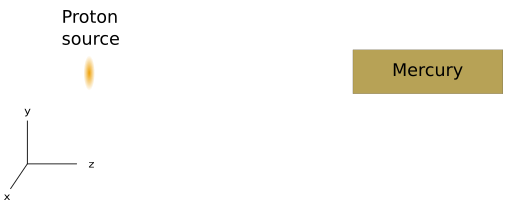
\includegraphics[scale=0.7]{../figs/mercury.png}
	\caption[VPI]{Planar view of Verification Problem I, 22 cm  x 44 cm x 186 cm}
	\label{fig:VPI}
\end{figure}
%
\begin{figure}[h!]
	\centering
	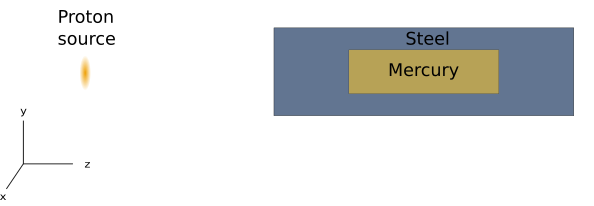
\includegraphics[scale=0.71]{../figs/mer_steel.png}
	\caption[VPI]{Planar view of Verification Problem II geometry, 44 cm x 88 cm x 372 cm}
	\label{fig:VPII}
\end{figure}
%
\subsection{Shut Down Dose Rate Workflow}
The patched, cell based and mesh based, \gls{dag}-\gls{mcnp}6.1 was used to
perform the neutron transport. The neutron flux and the radionuclide
information were collected on a geometric volume, a 1x1x1 mesh, a 2x2x2 mesh,
and a 4x4x4 mesh. All meshes were uniformly distributed Cartesian meshes. In
addition, each geometry was divided into 8 and 64 equal parts. Dividing up the
geometry allowed for direct comparison to the mesh. It is important to note
that Verification problem II required materials to be mixed when the geometry
was divided into 8 equal parts as the division does not align with the geometric
volumes in the original problem.
Next, an activation calculation was performed on each of the geometric cells
using a perl script previously written for cell based workflow. An activation
calculation was also performed per voxel in each of the meshes, automated by
the python script.
A photon source script was then used to collect output from CINDER90 to
build a photon source card, \emph{sdef}, in the case of the cell based workflow.
In the case of the mesh based workflow, another source script was used to
build a photon source \gls{moab} file which can be used in lieu of a source card
in the photon transport.
In all cases, the biological dose rate was collected in a superimposed
Cartesian mesh by applying flux-to-dose conversion factors to the photon flux.
%
\subsection{Results}
\subsubsection{Verification Problem I}
The \emph{rnucs} tally collected information on production and destruction of
isotopes during the neutron transport step. This information was collected
in the mercury volume, using the cell based \gls{sdr}-rnucs workflow;
in each of the previously mentioned meshes, using the new mesh based
\gls{sdr}-rnucs workflow; and on each volumetric cell of the subdivided
geometry, using the cell based \gls{sdr}-rnucs workflow.\\
Figure \ref{fig:1prod_cell_1x_2x_4x} shows the radionuclide production information
collected in the mercury volume, the 1x1x1 mesh, and the sum of the results in
each voxel for the 2x2x2 and 4x4x4 meshes. The bottom graph in Figure
\ref{fig:1prod_cell_1x_2x_4x} shows the relative change between each mesh and the
mercury volume.
The relative change, between the information collected in the Cartesian mesh and
mercury volume, is small or zero. There are a few isotopes that
have a some relative change, but even these isotopes are not statistically different.
%
\begin{figure}[H]
	\centering
	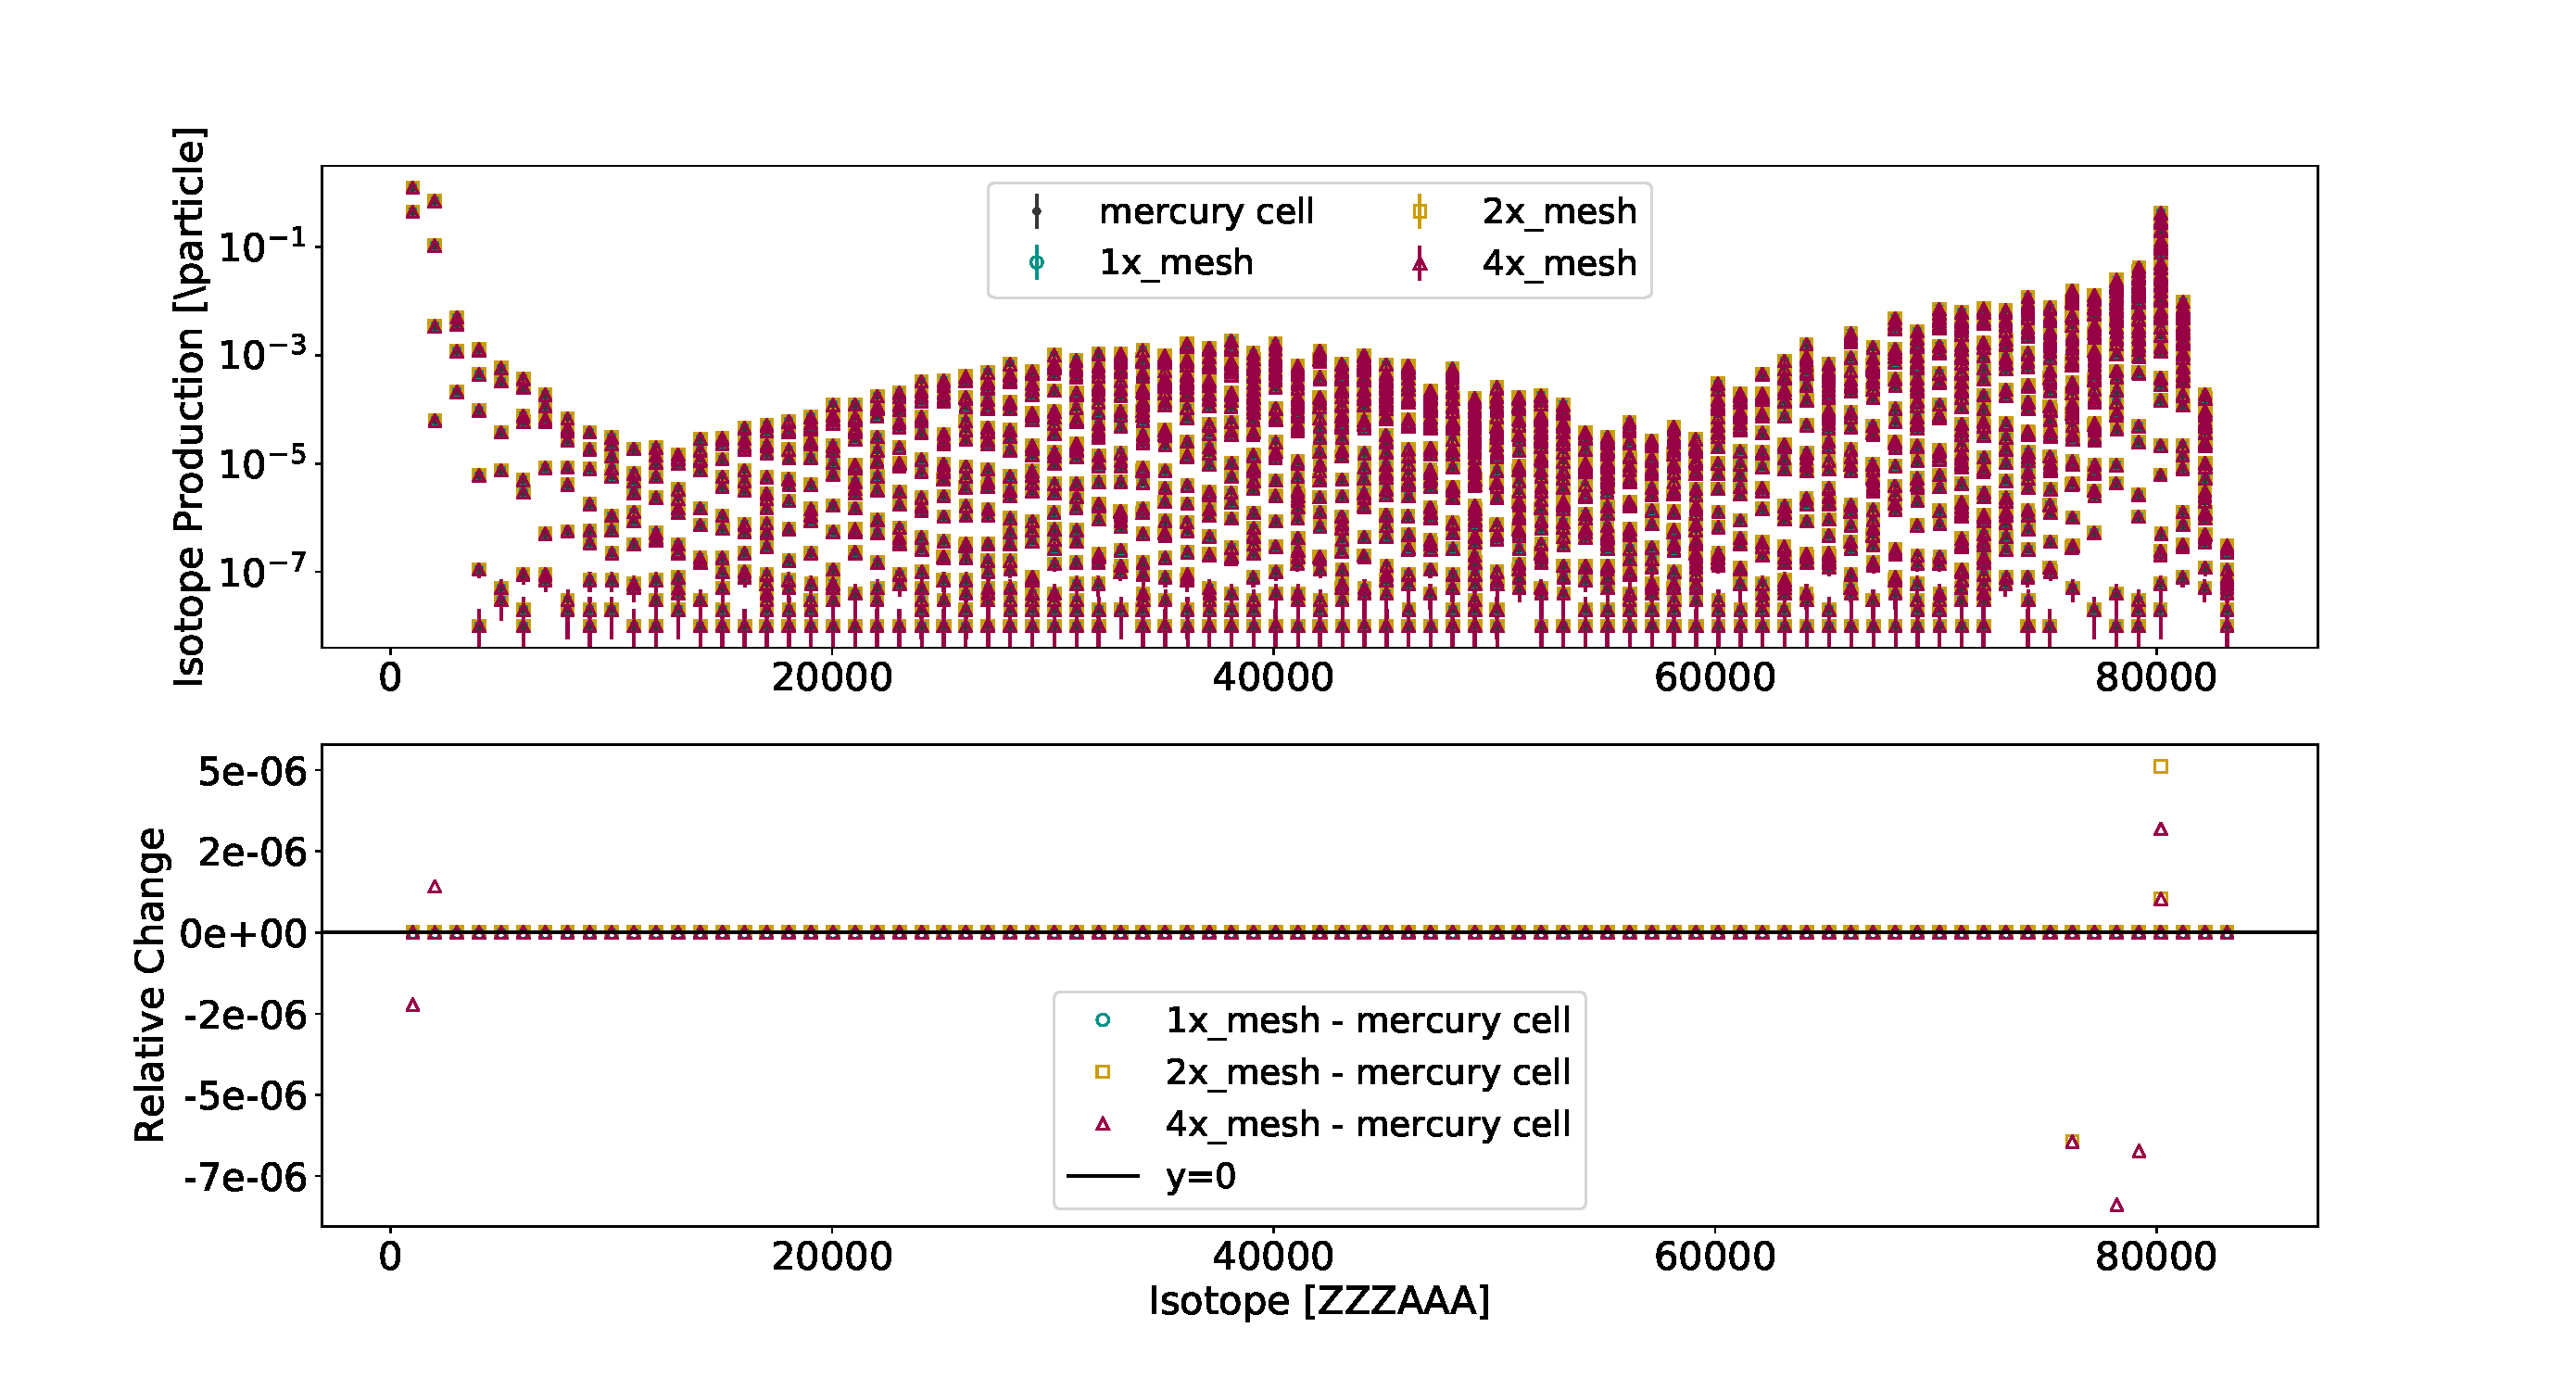
\includegraphics[scale=0.4,trim={2cm 1cm 3cm 2cm},clip]{../figs/toy_p1/prod_VPI_1x_2x_4x.pdf}
	\caption{Radionuclide production comparison for mercury cell and different meshes}
	\label{fig:1prod_cell_1x_2x_4x}
\end{figure}
%
Figure \ref{fig:1prod_cell_2x} compares the results collected in the mercury
volume, the summed up results of the 2x2x2 mesh and the 2x2x2 divided geometry. In
this graph, the relative change for certain isotopes is significantly large.
In order to access this, the absolute
relative change between the divided geometry and original geometry was compared
to the isotope production results obtained in the mercury volume.
Figure \ref{fig:1prod_cell_2x_rc} shows the relative change is large when the
isotope production per particle is low. This suggests that the differences can
be minimized with more histories run.
%
\begin{figure}[H]
	\centering
	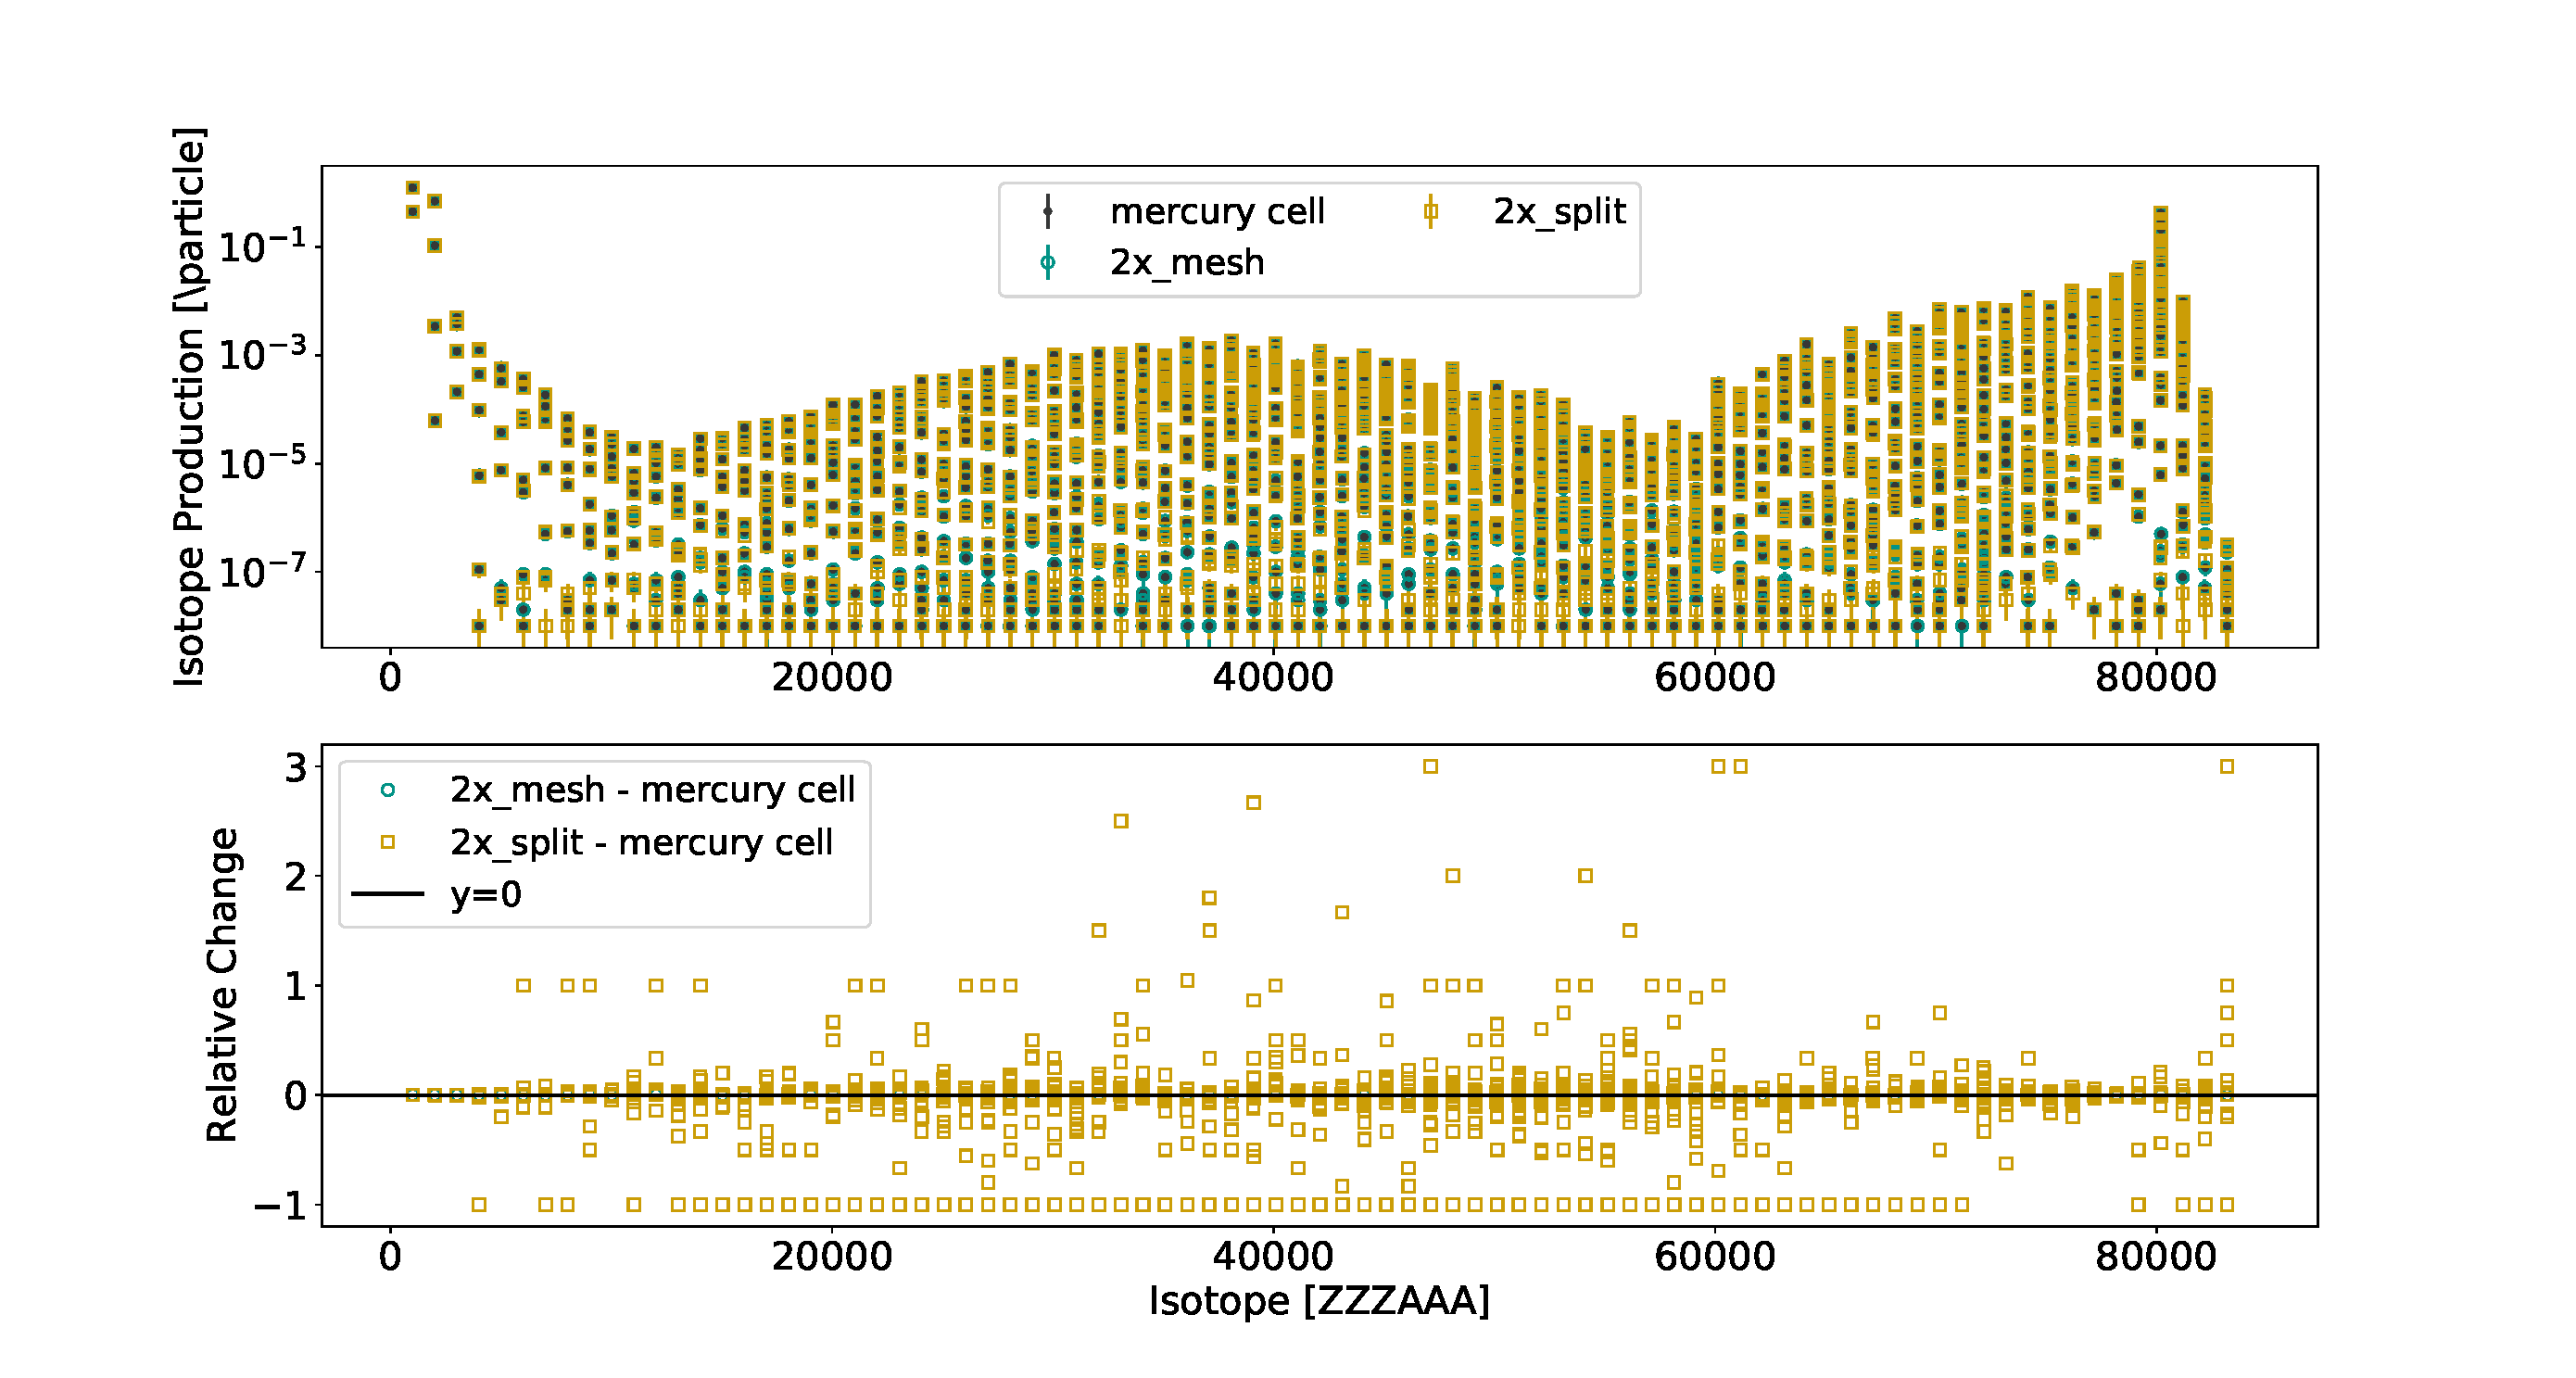
\includegraphics[scale=0.4,trim={2cm 1cm 3cm 2cm},clip]{../figs/toy_p1/prod_VPI_2x.pdf}
	\caption{Radionuclide production comparison between mercury cell, 2x2x2 mesh and geometry split}
	\label{fig:1prod_cell_2x}
\end{figure}
%
\begin{figure}[H]
	\centering
	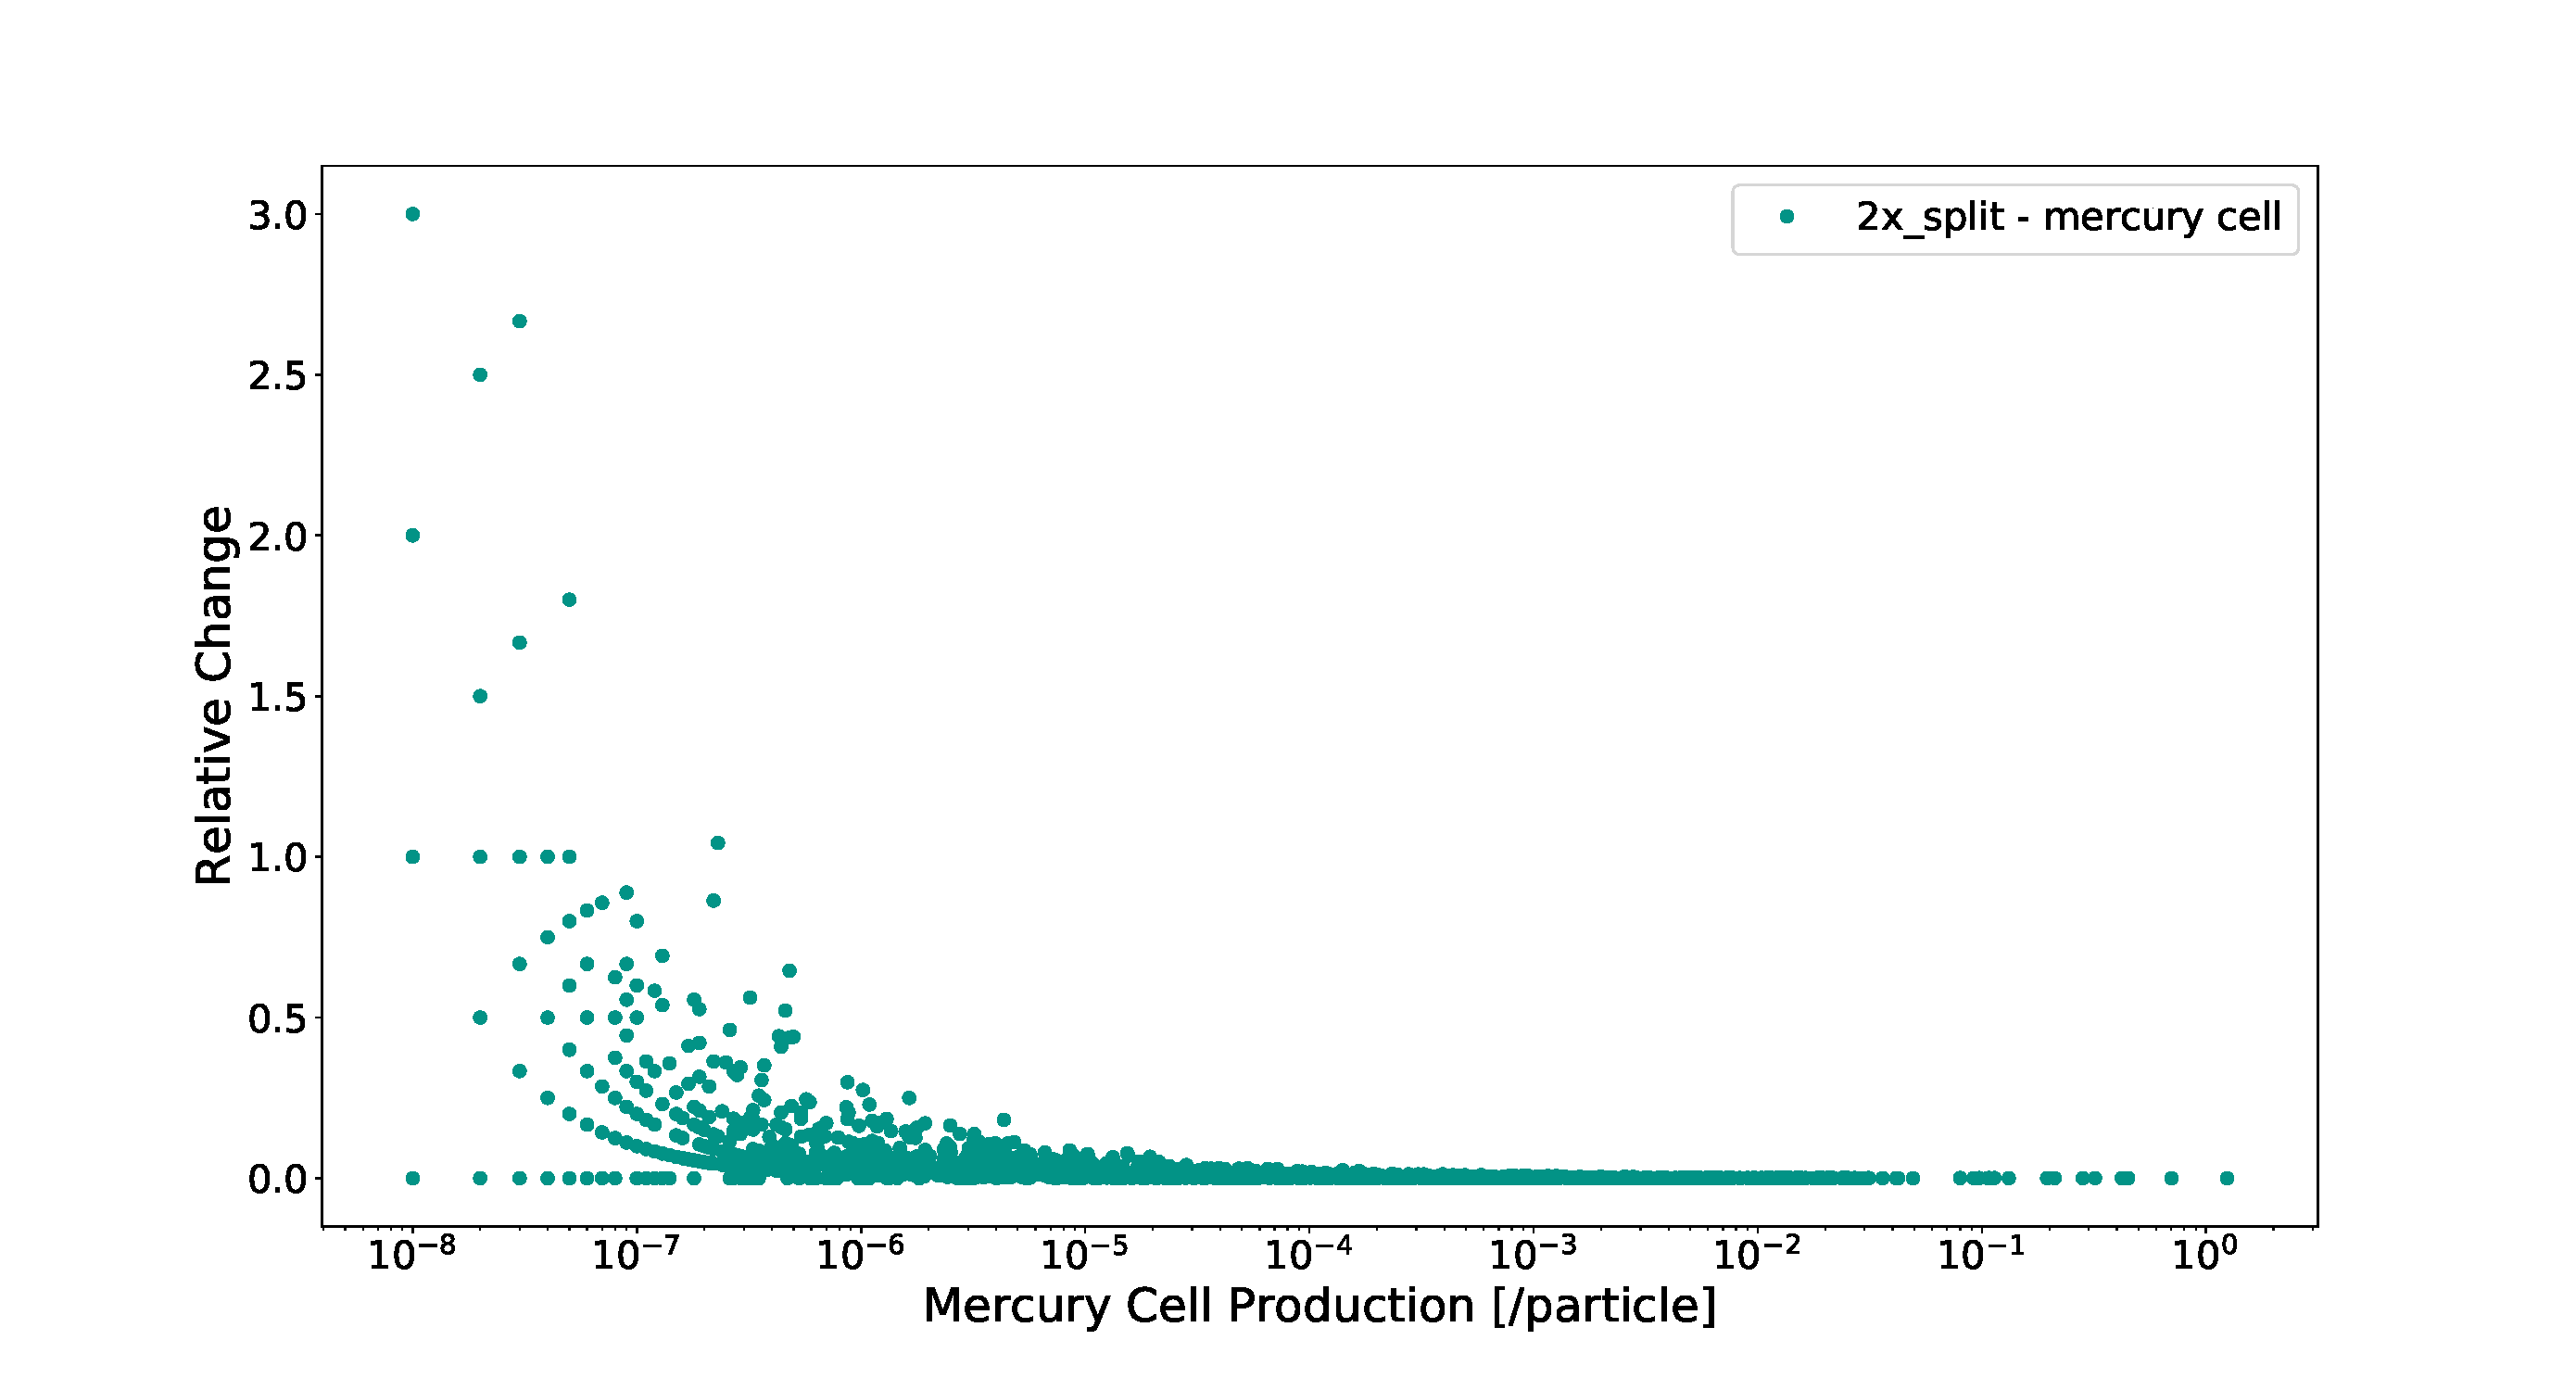
\includegraphics[scale=0.35,trim={3cm 0.5cm 4.5cm 3cm},clip]{../figs/toy_p1/prod_VPI_rc_2x_split.pdf}
	\caption{Relative change between mercury cell and 2x2x2 geometry split vs. the isotope production of the mercury cell}
	\label{fig:1prod_cell_2x_rc}
\end{figure}

A similar comparison can be seen for the 4x4x4 mesh and the 4x4x4 divided
geometry in Figure \ref{fig:1prod_cell_4x}. The behavior of the relative change
is similar to that of the 2x2x2 divided geometry. A graph comparing the relative
change between the divided geometry and the original geometry to the isotope
production results obtained in the mercury volume can be seen in Figure
\ref{fig:1prod_cell_4x_rc}.
%
\begin{figure}[H]
	\centering
	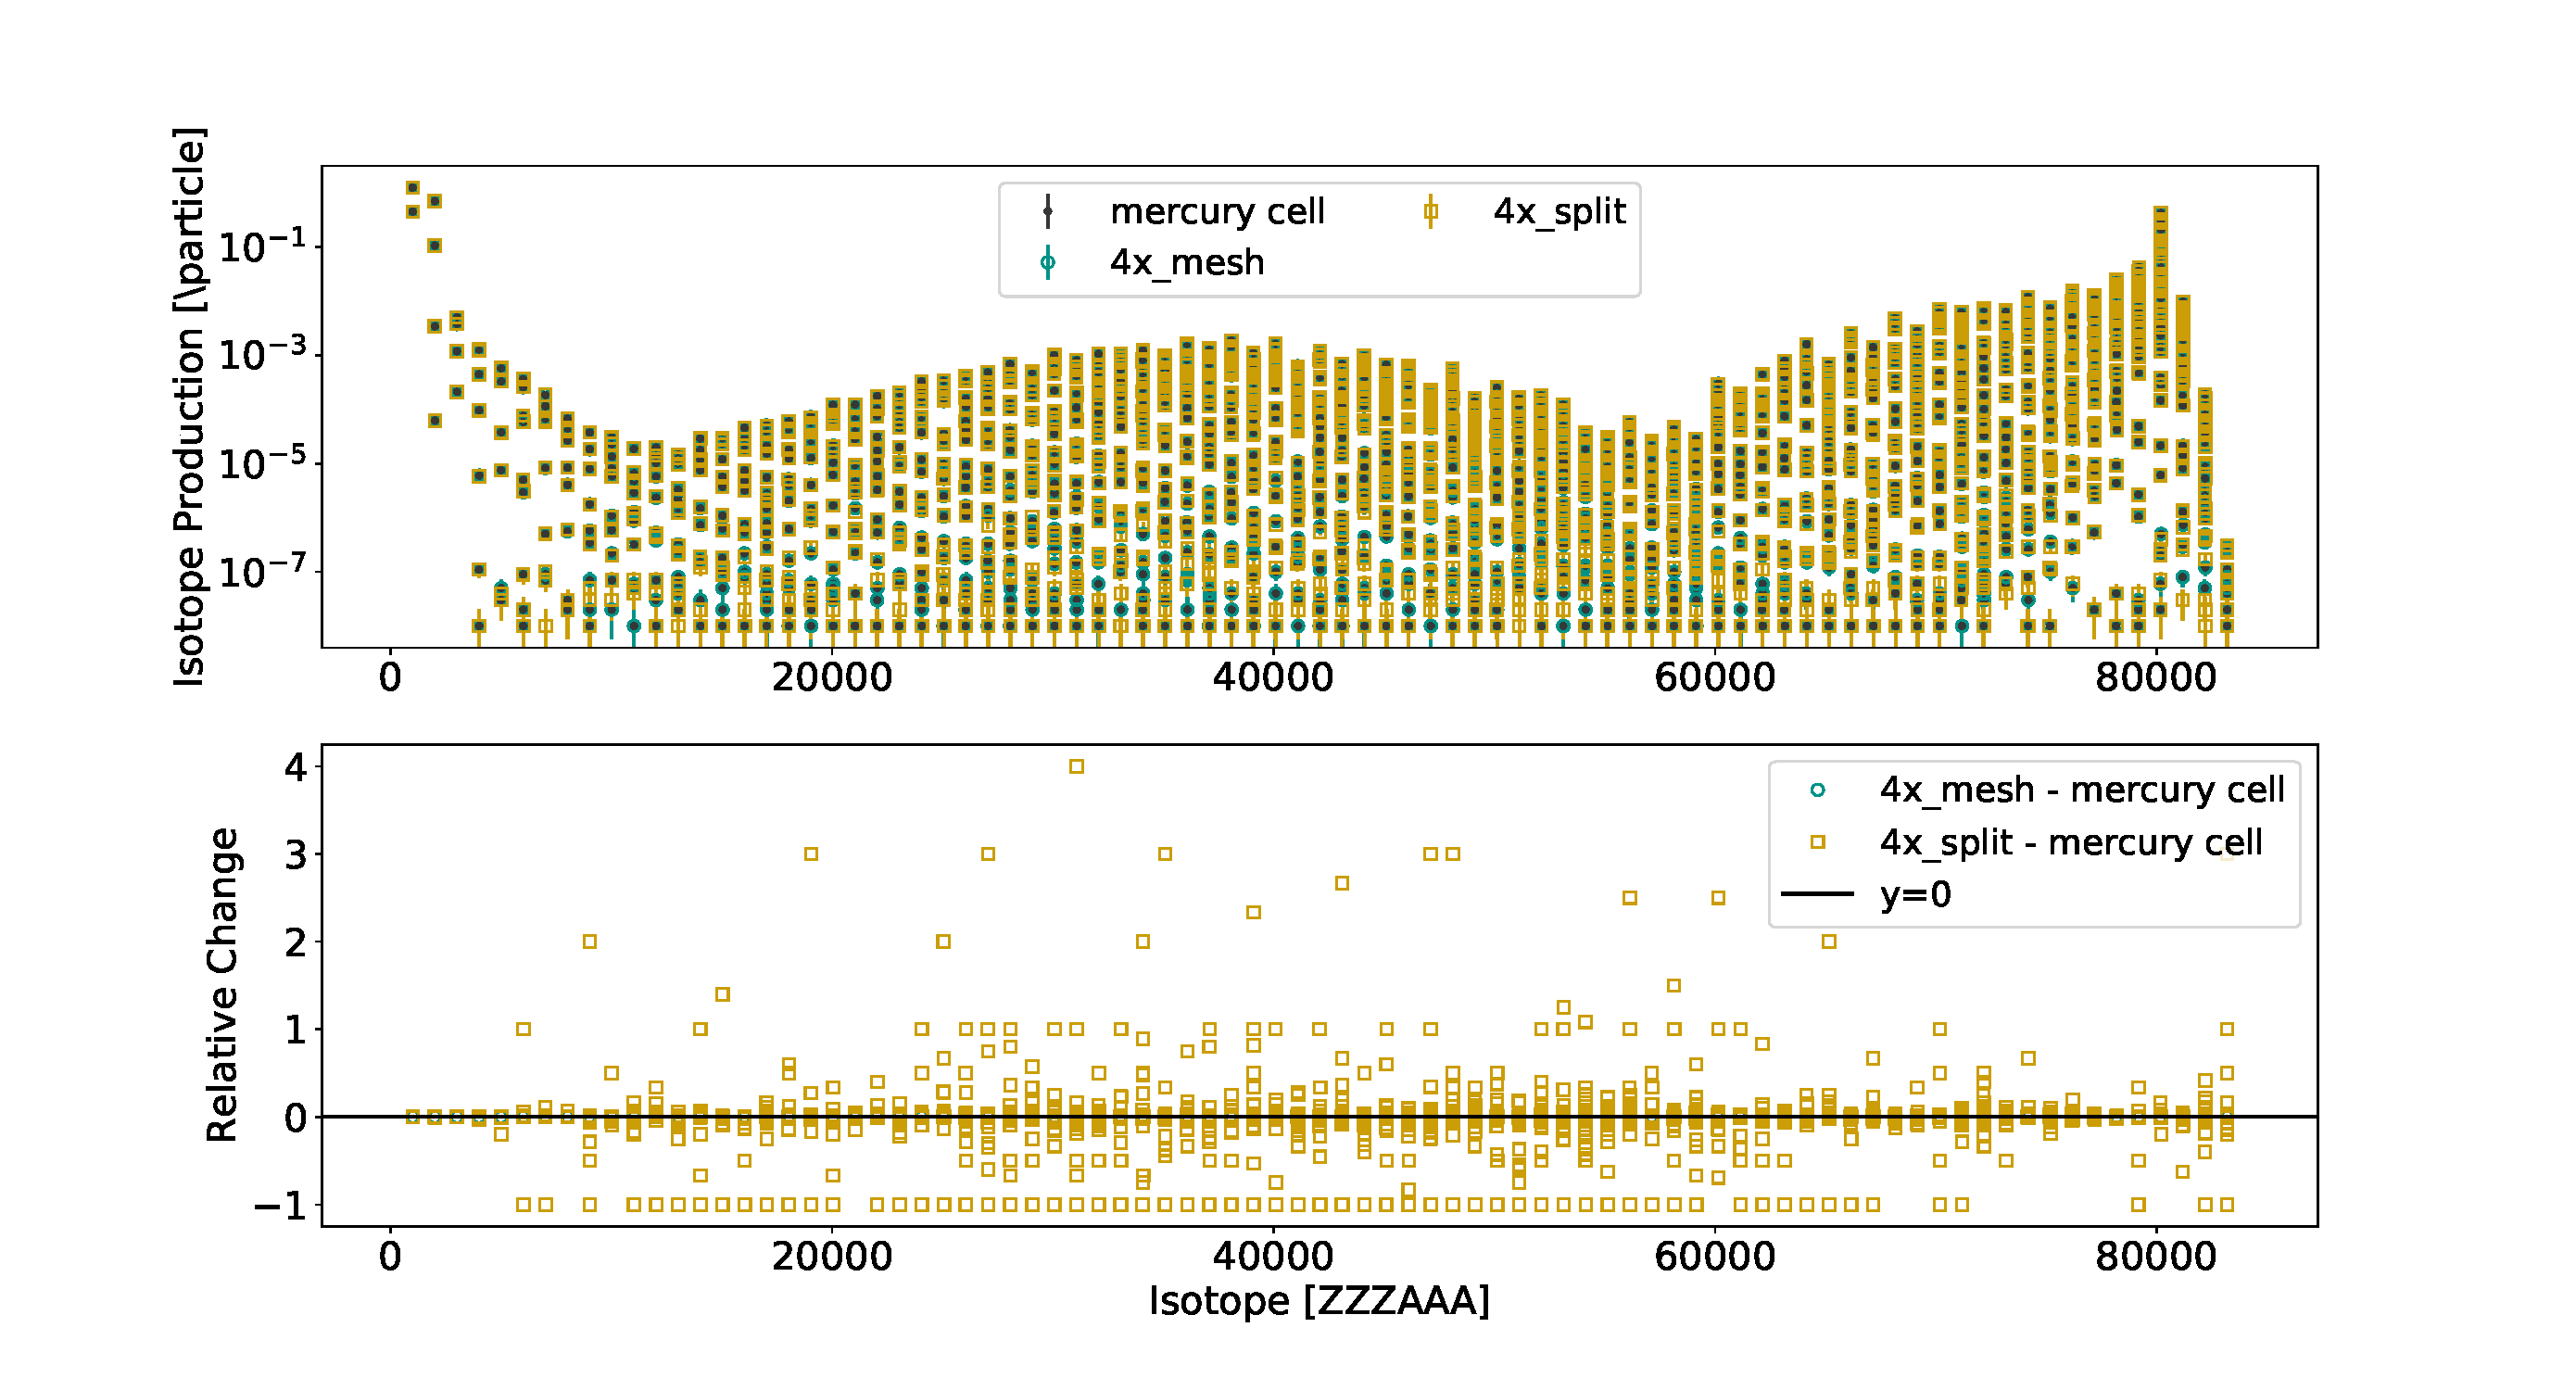
\includegraphics[scale=0.4,trim={2cm 1cm 3cm 2cm},clip]{../figs/toy_p1/prod_VPI_4x.pdf}
	\caption{Radionuclide production comparison between mercury cell, 4x4x4 mesh and geometry split}
	\label{fig:1prod_cell_4x}
\end{figure}
%
\begin{figure}[H]
 \centering
 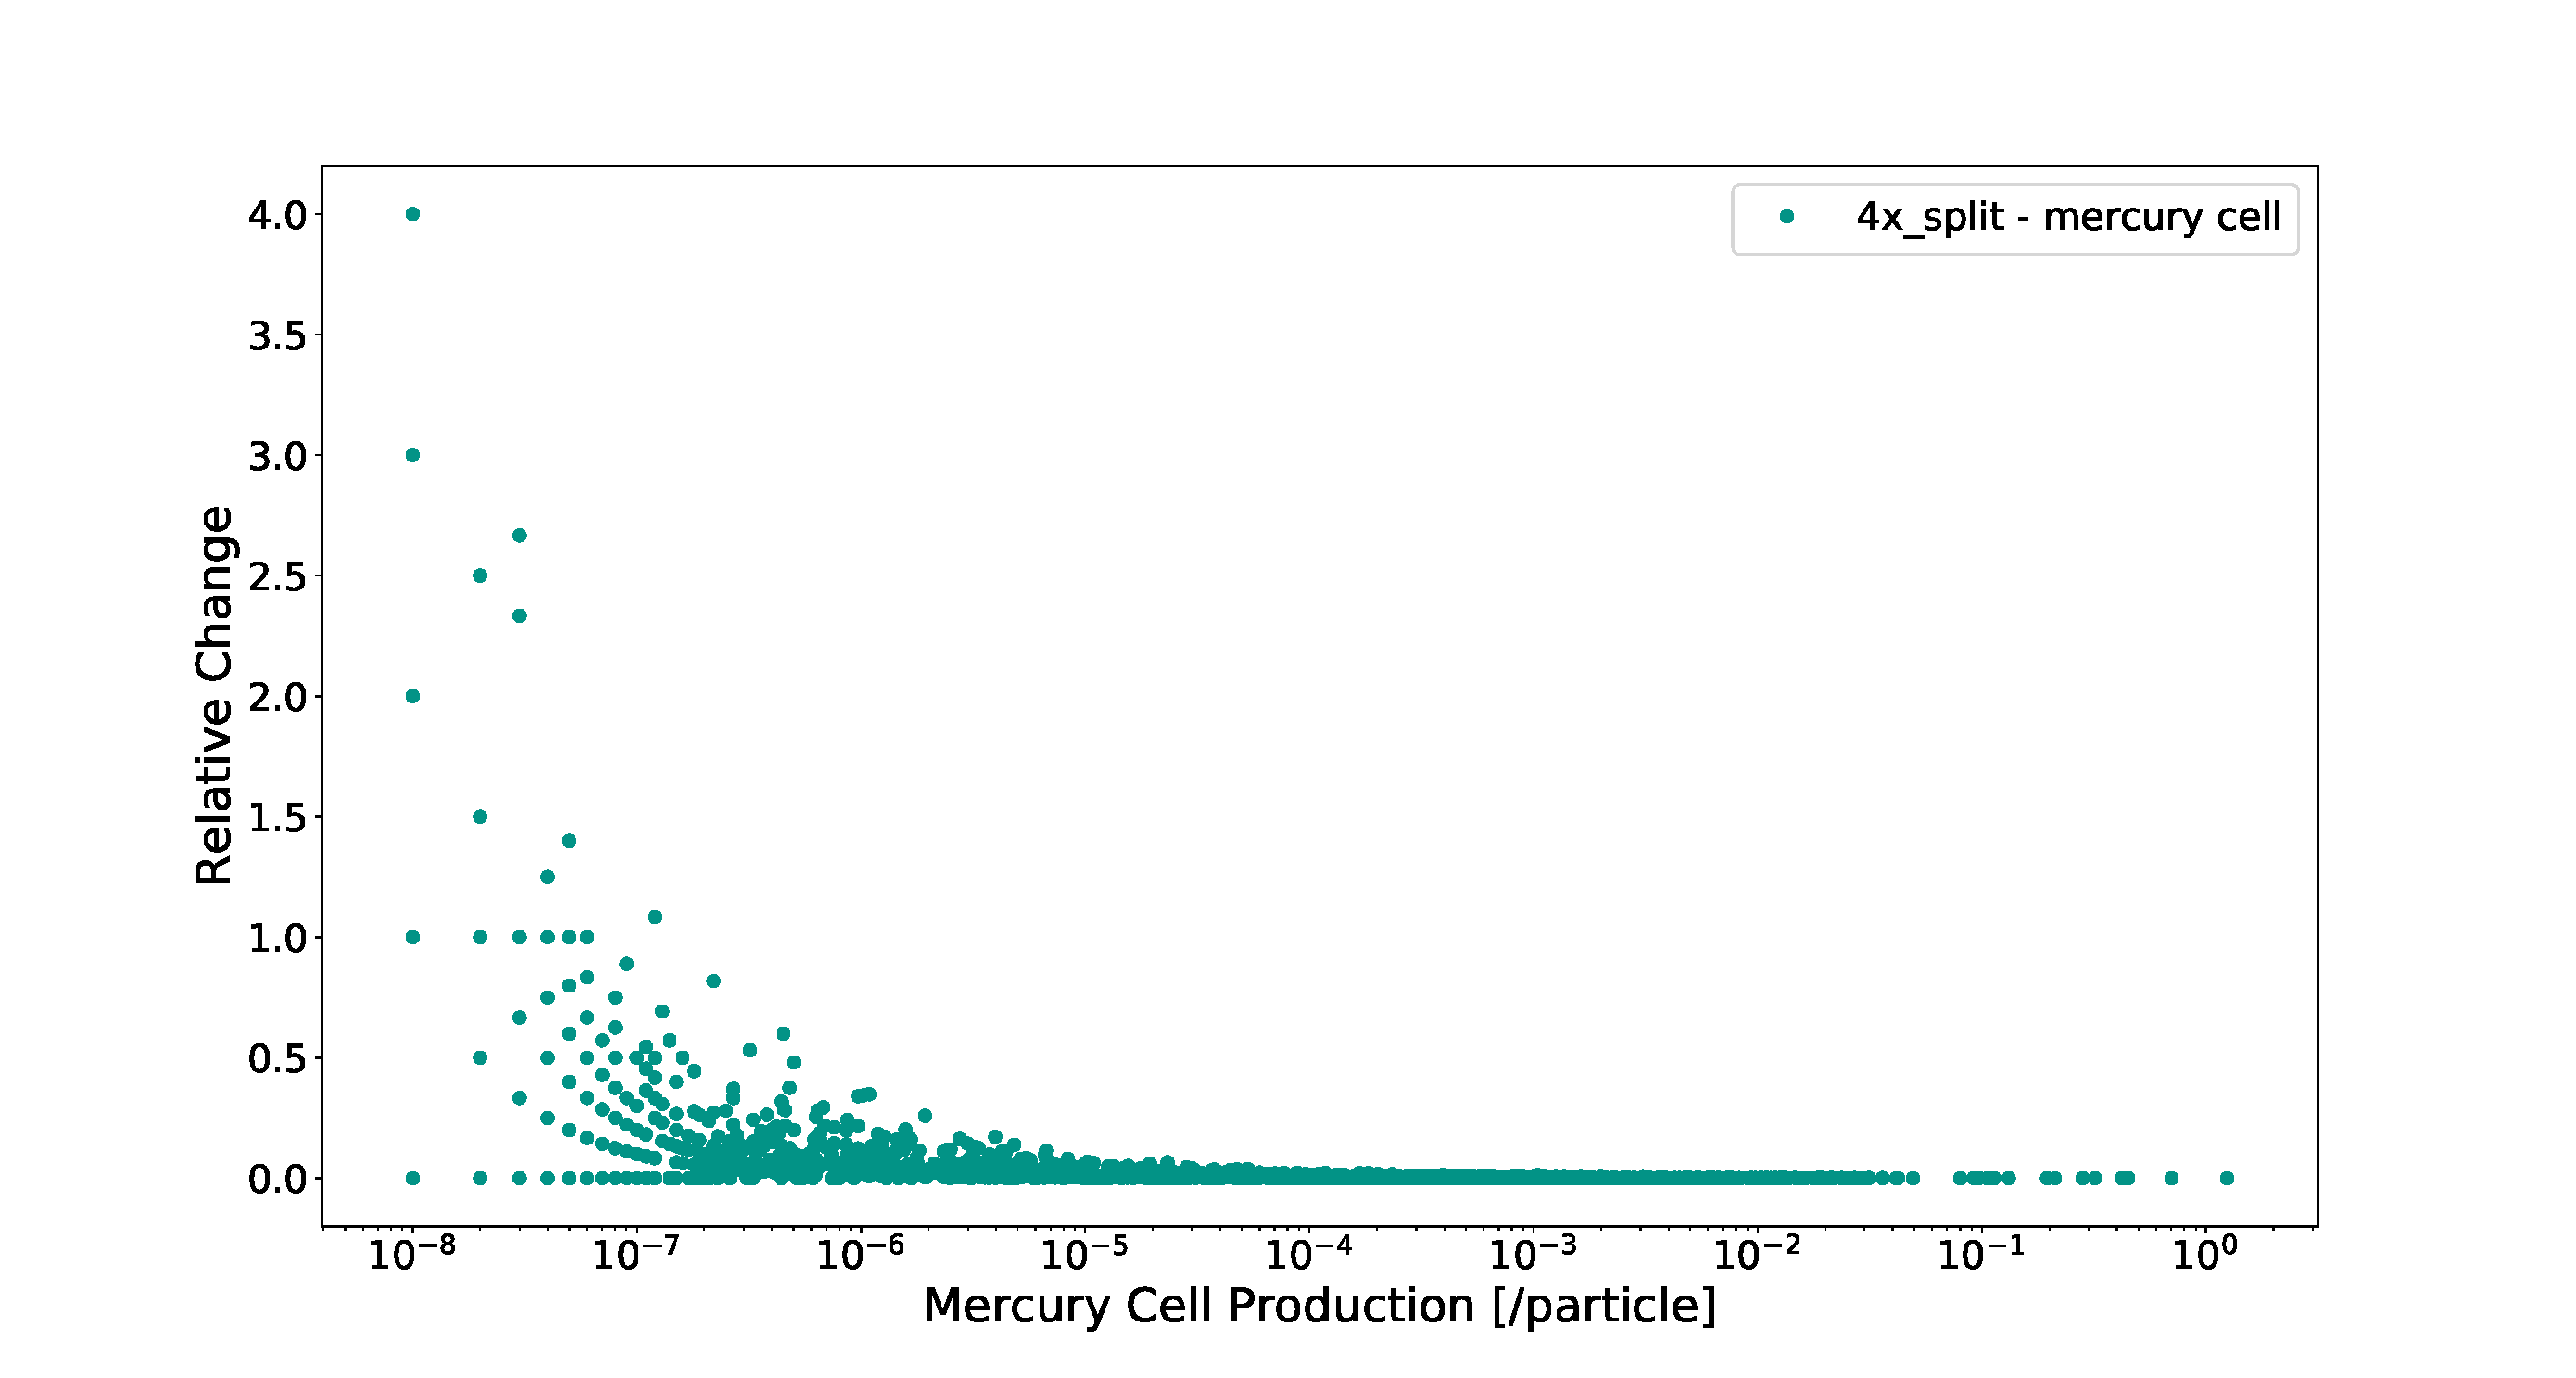
\includegraphics[scale=0.35,trim={3cm 0.5cm 4.5cm 3cm},clip]{../figs/toy_p1/prod_VPI_rc_4x_split.pdf}
 \caption{Relative change between mercury cell and 4x4x4 geometry split vs. the isotope production of the mercury cell}
 \label{fig:1prod_cell_4x_rc}
\end{figure}
%
Next, the photon emission density was collected during the activation step of
the workflow. The photon emission density was collected for the original
mercury volume, each of the meshes covering the mercury volume, and on each of
the volumes of the divided geometry.
Figure \ref{fig:1spec_cell_1x_2x_4x} shows the photon emission density
collected in the mercury volume, and the average photon emission density
found in the different meshes. The bottom graph of Figure
\ref{fig:1spec_cell_1x_2x_4x} shows the relative change between the mesh and
the mercury volume. This graph suggests that the results are not significantly
different.
%
\begin{figure}[H]
 \centering
 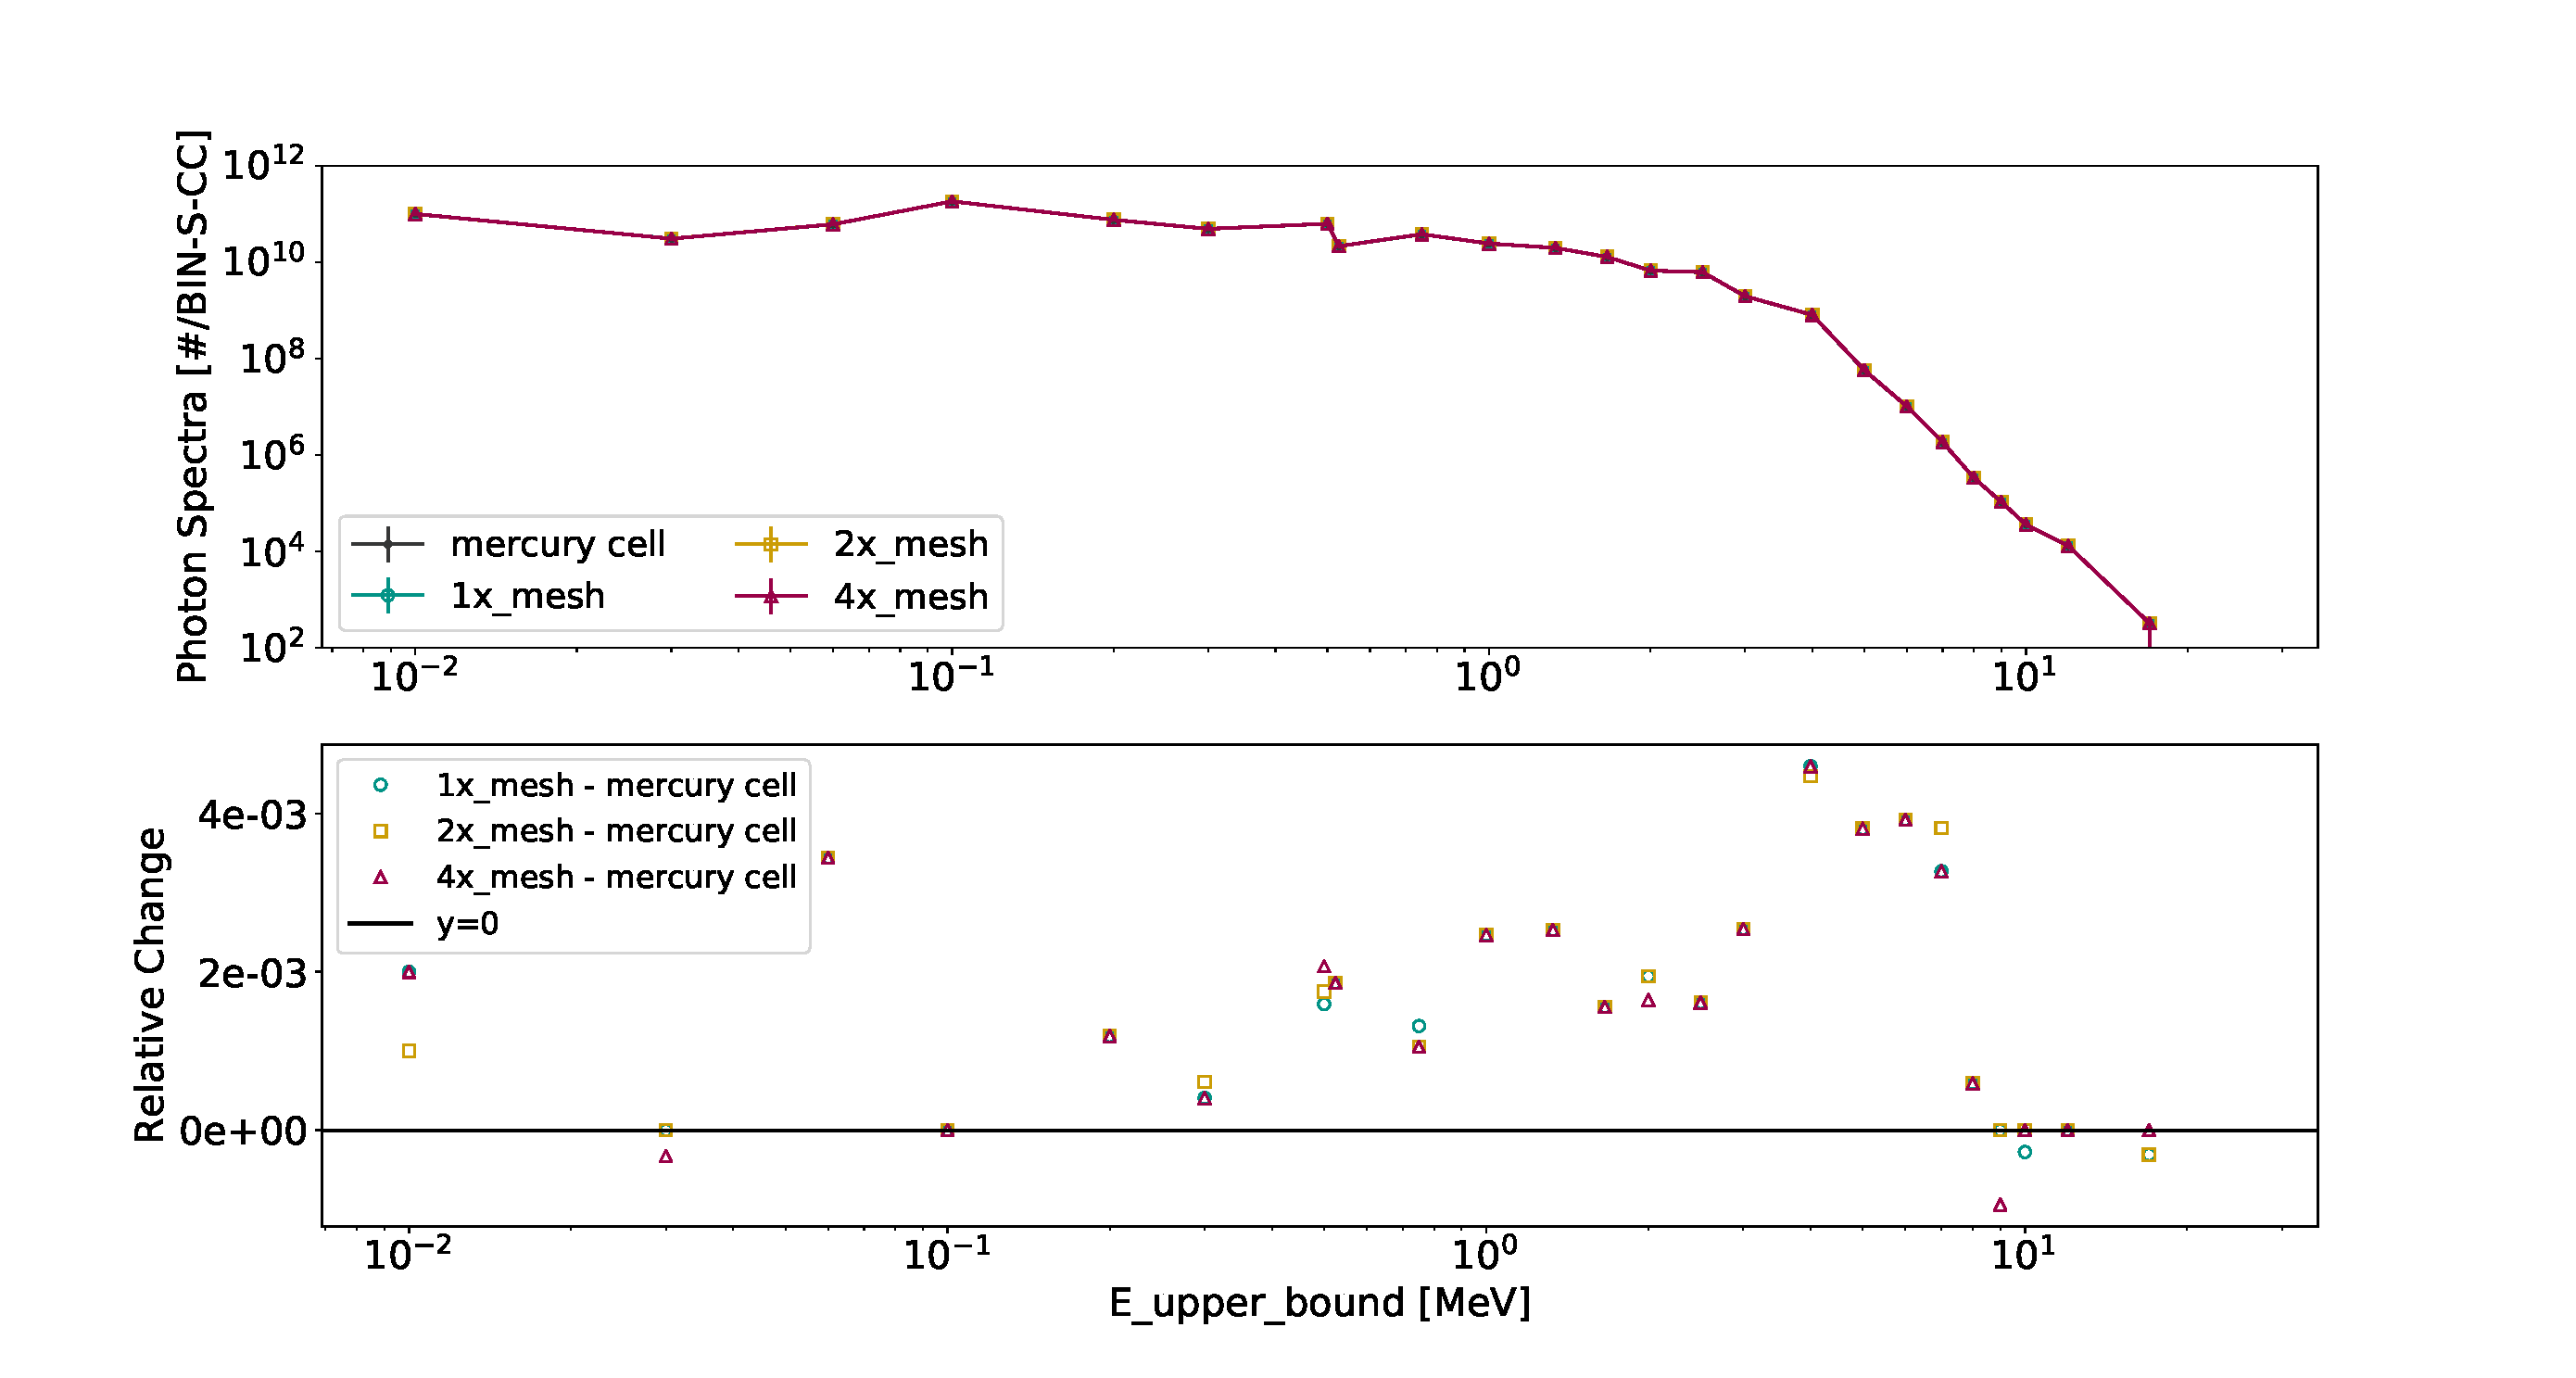
\includegraphics[scale=0.4,trim={2cm 0.5cm 3cm 2cm},clip]{../figs/toy_p1/spec_VPI_1x_2x_4x.pdf}
 \caption{Photon Spectrum in mercury cell and different meshes}
 \label{fig:1spec_cell_1x_2x_4x}
\end{figure}
%
Figure \ref{fig:1spec_cell_2x} shows the photon emission density for the
original volume, the 2x2x2 mesh, and the 2x2x2 divided geometry. The results
shown for the mesh and the divided geometry are the average results of all the
voxels or volumes spanning the same physical space. The bottom graph shows the
relative change of the
divided geometry and the original mercury volume, and between the mesh and the
original mercury volume.
A similar graph can be seen in Figure \ref{fig:1spec_cell_4x} showing results
for the 4x4x4 mesh and 4x4x4 divided geometry.
Neither of these comparison show much difference between results. This
strengthens the earlier hypothesis that isotopes with really small production
rates do not significantly contribute to the photon emission.
%
\begin{figure}[H]
 \centering
 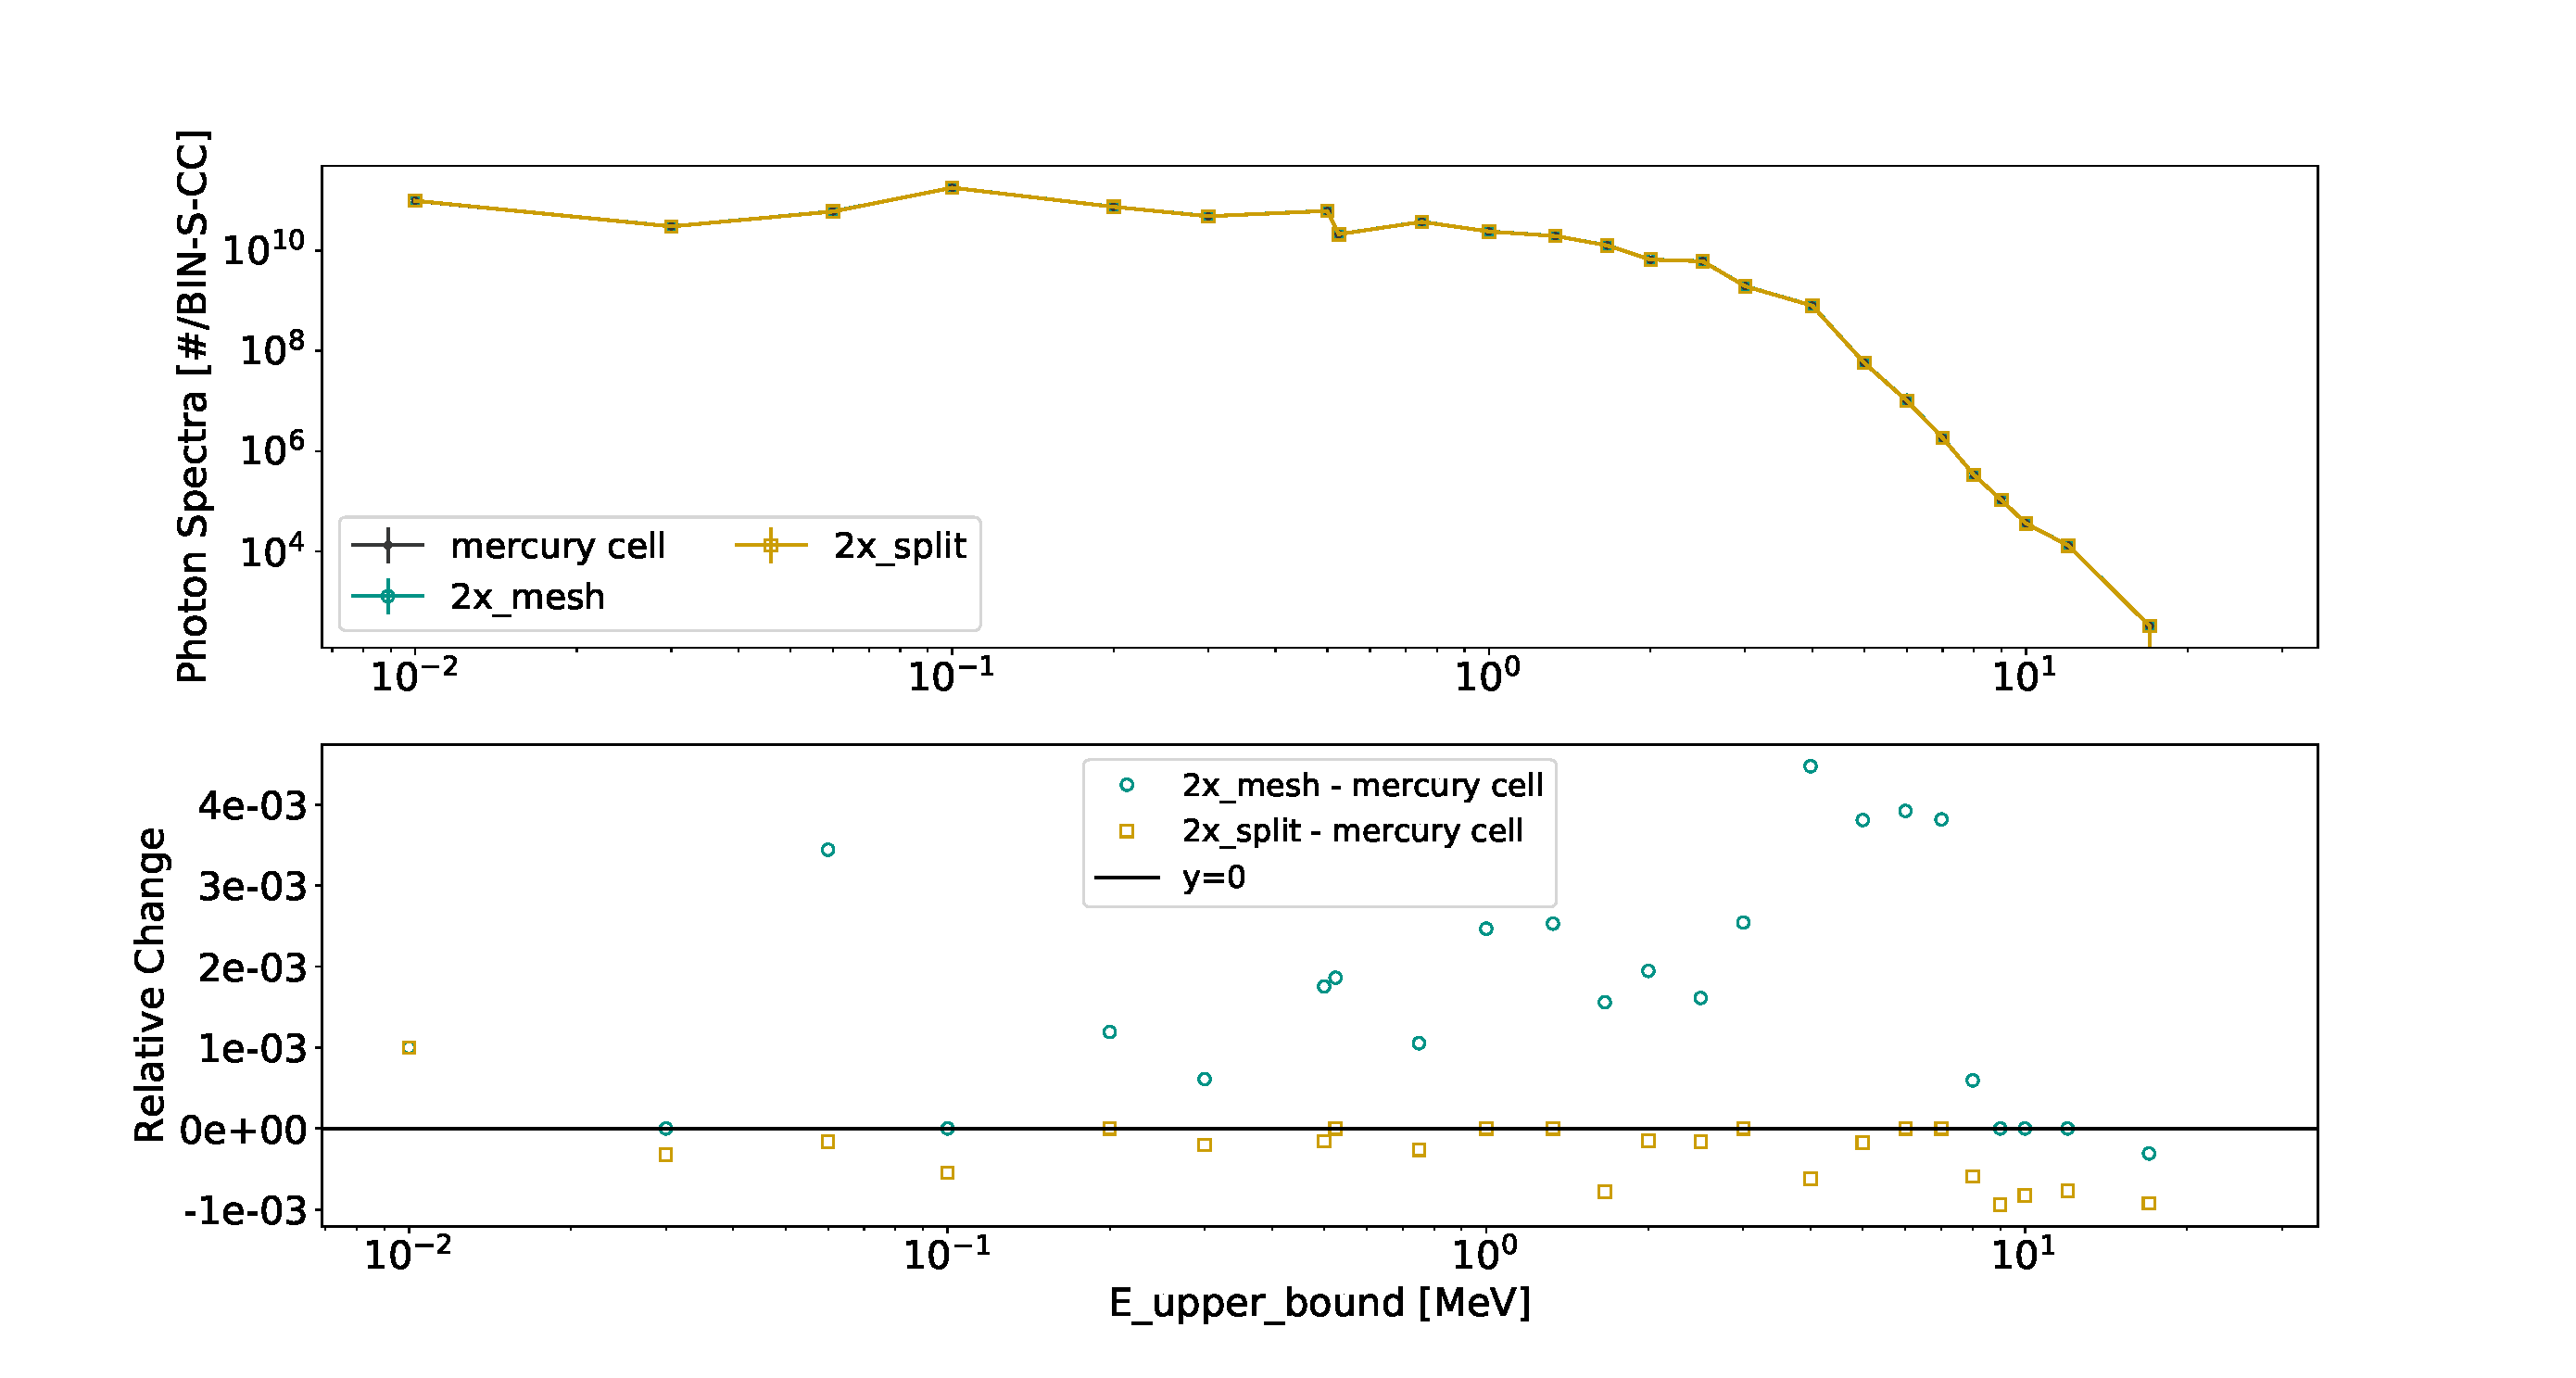
\includegraphics[scale=0.4,trim={2cm 0.5cm 3cm 2cm},clip]{../figs/toy_p1/spec_VPI_2x.pdf}
 \caption{Photon Spectrum in mercury cell, 2x2x2 mesh, and geometry split}
 \label{fig:1spec_cell_2x}
\end{figure}
\begin{figure}[H]
 \centering
 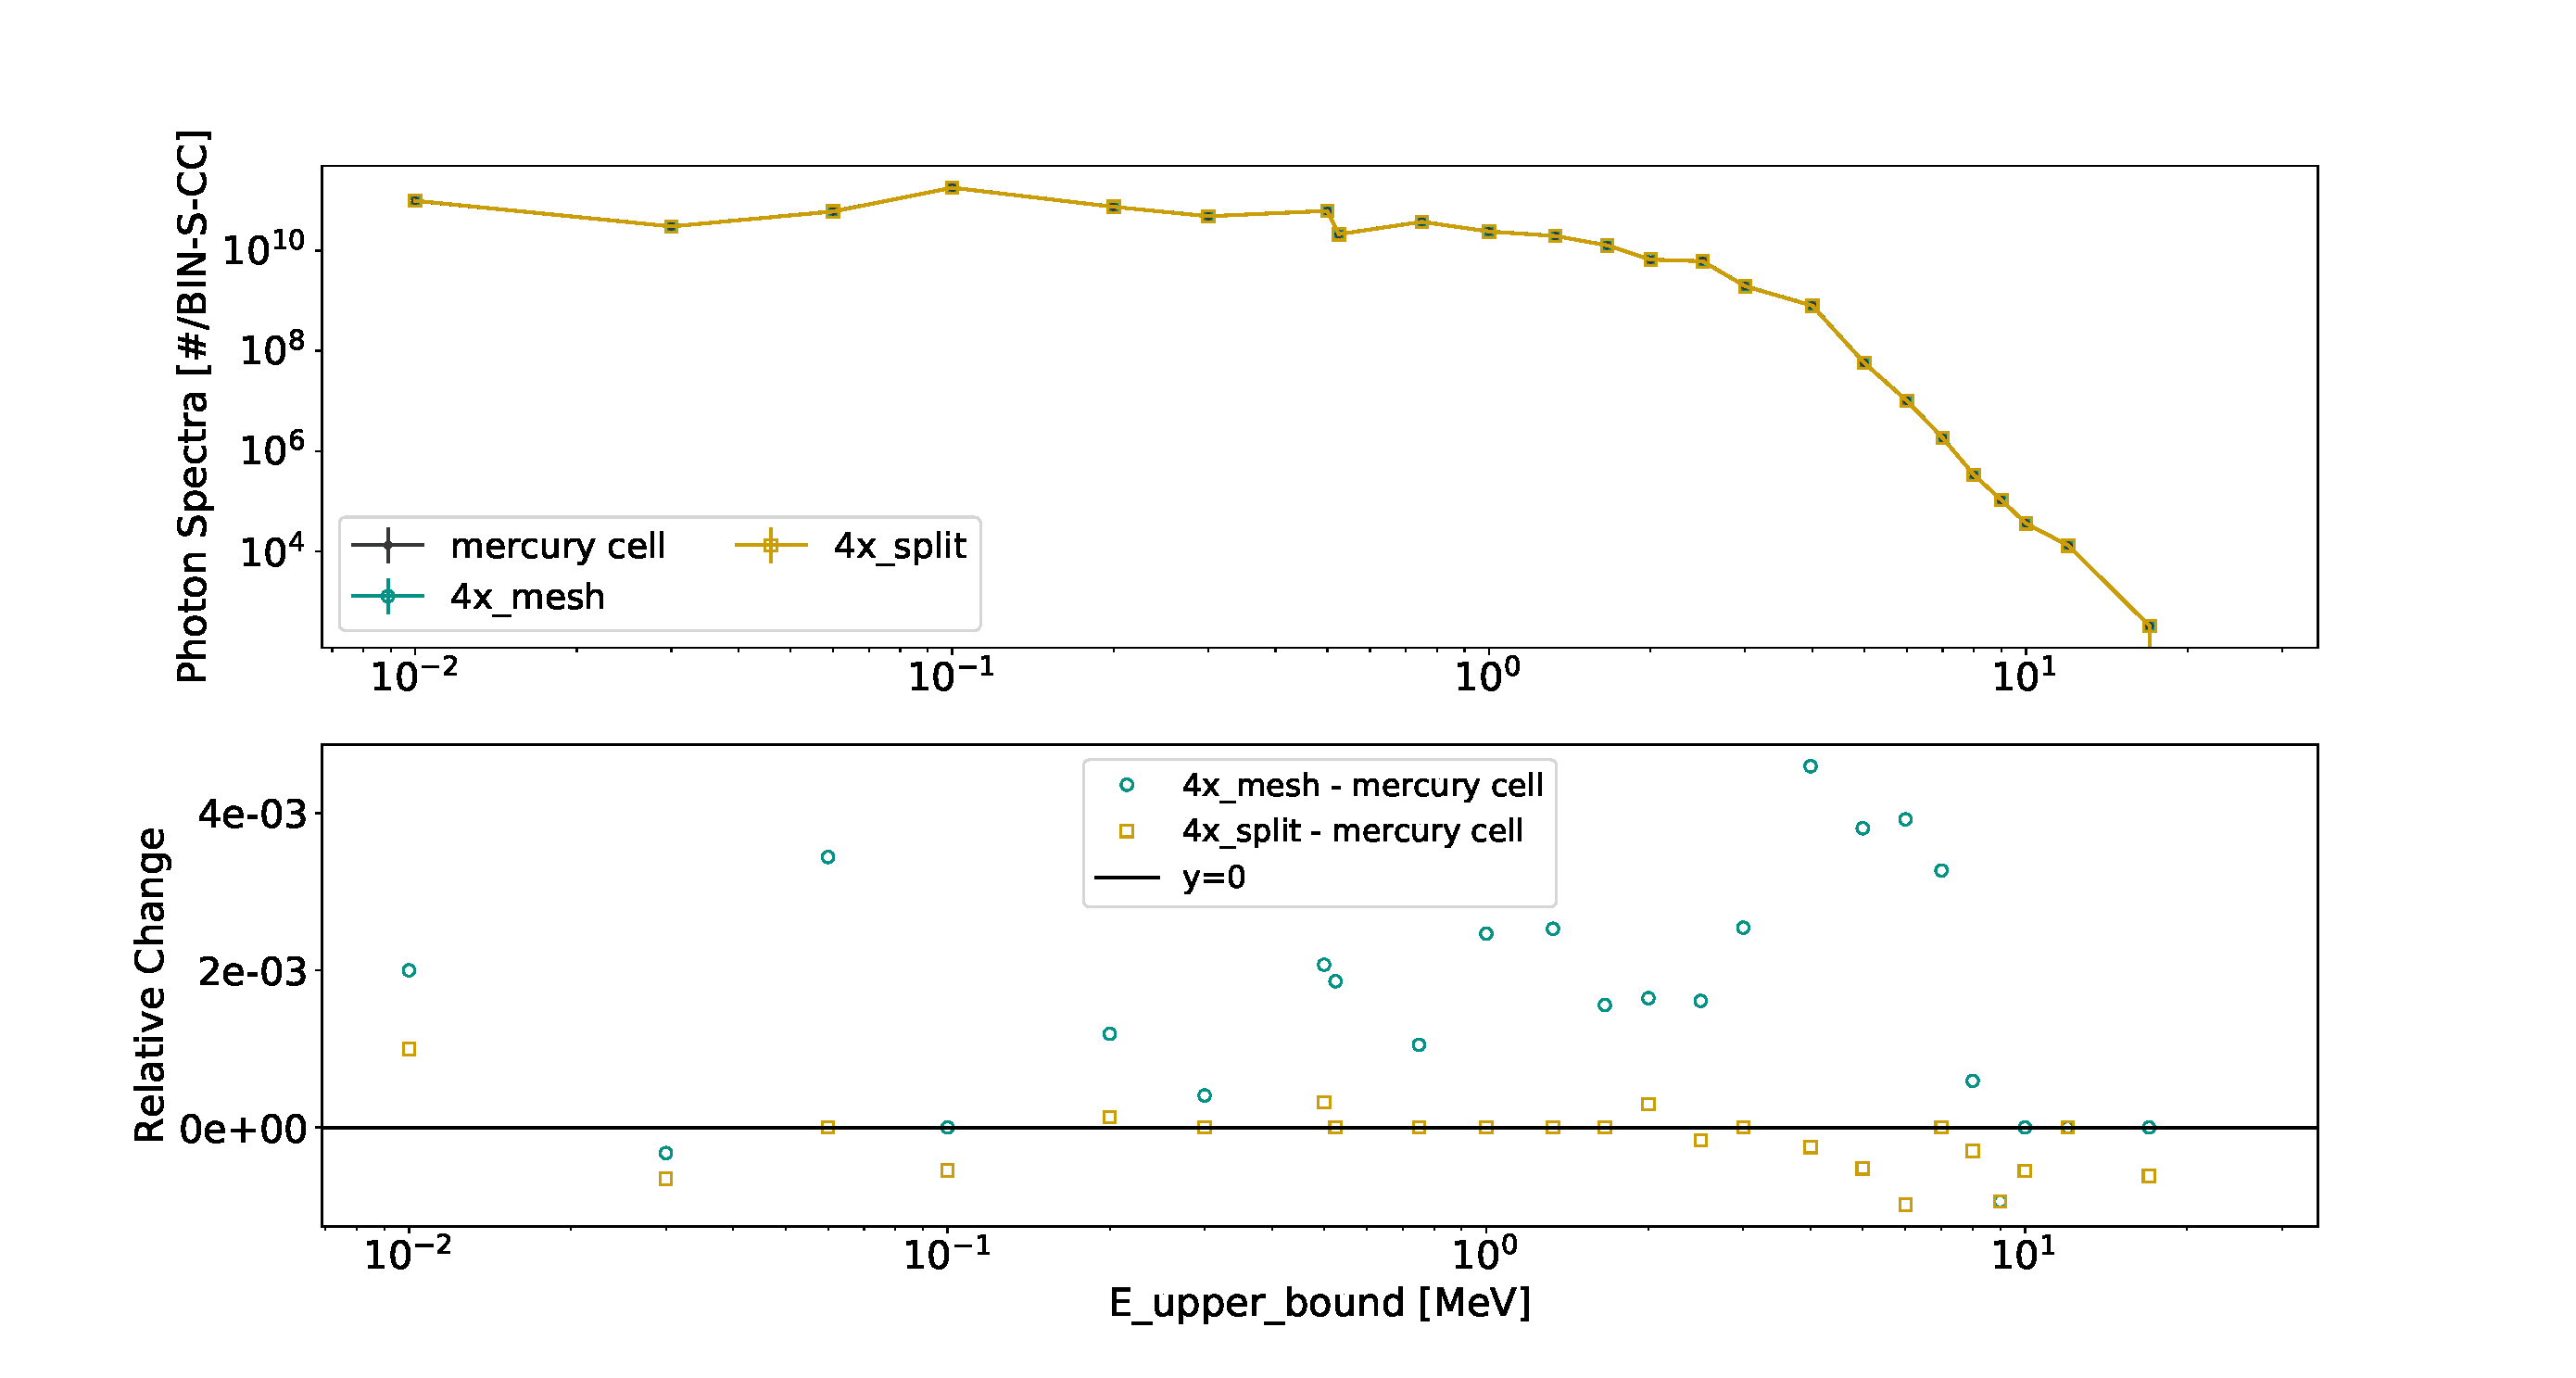
\includegraphics[scale=0.4,trim={2cm 0.5cm 3cm 2cm},clip]{../figs/toy_p1/spec_VPI_4x.pdf}
 \caption{Photon Spectrum in mercury cell, 4x4x4 mesh, and geometry split}
 \label{fig:1spec_cell_4x}
\end{figure}
%
Figure \ref{fig:1spec_8v} shows the photon emission density per voxel for a
2x2x2 mesh and for the mercury volume. This graph shows higher photon emission
density for voxels 1, 3, 5, and 7 which are the voxels closer to the proton
source.
\begin{figure}[H]
	\begin{subfigure}[t]{1.0\textwidth}
		\hfill
		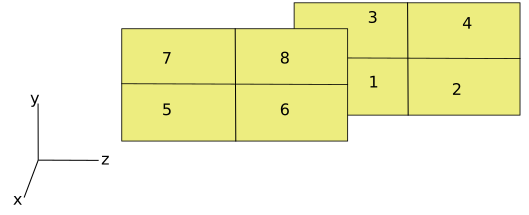
\includegraphics[scale=0.4, trim={0cm 0cm 0cm 0cm},clip]{../figs/voxels.png}
	\end{subfigure}\hfill
	\begin{subfigure}[t]{1.0\textwidth}
		\centering
		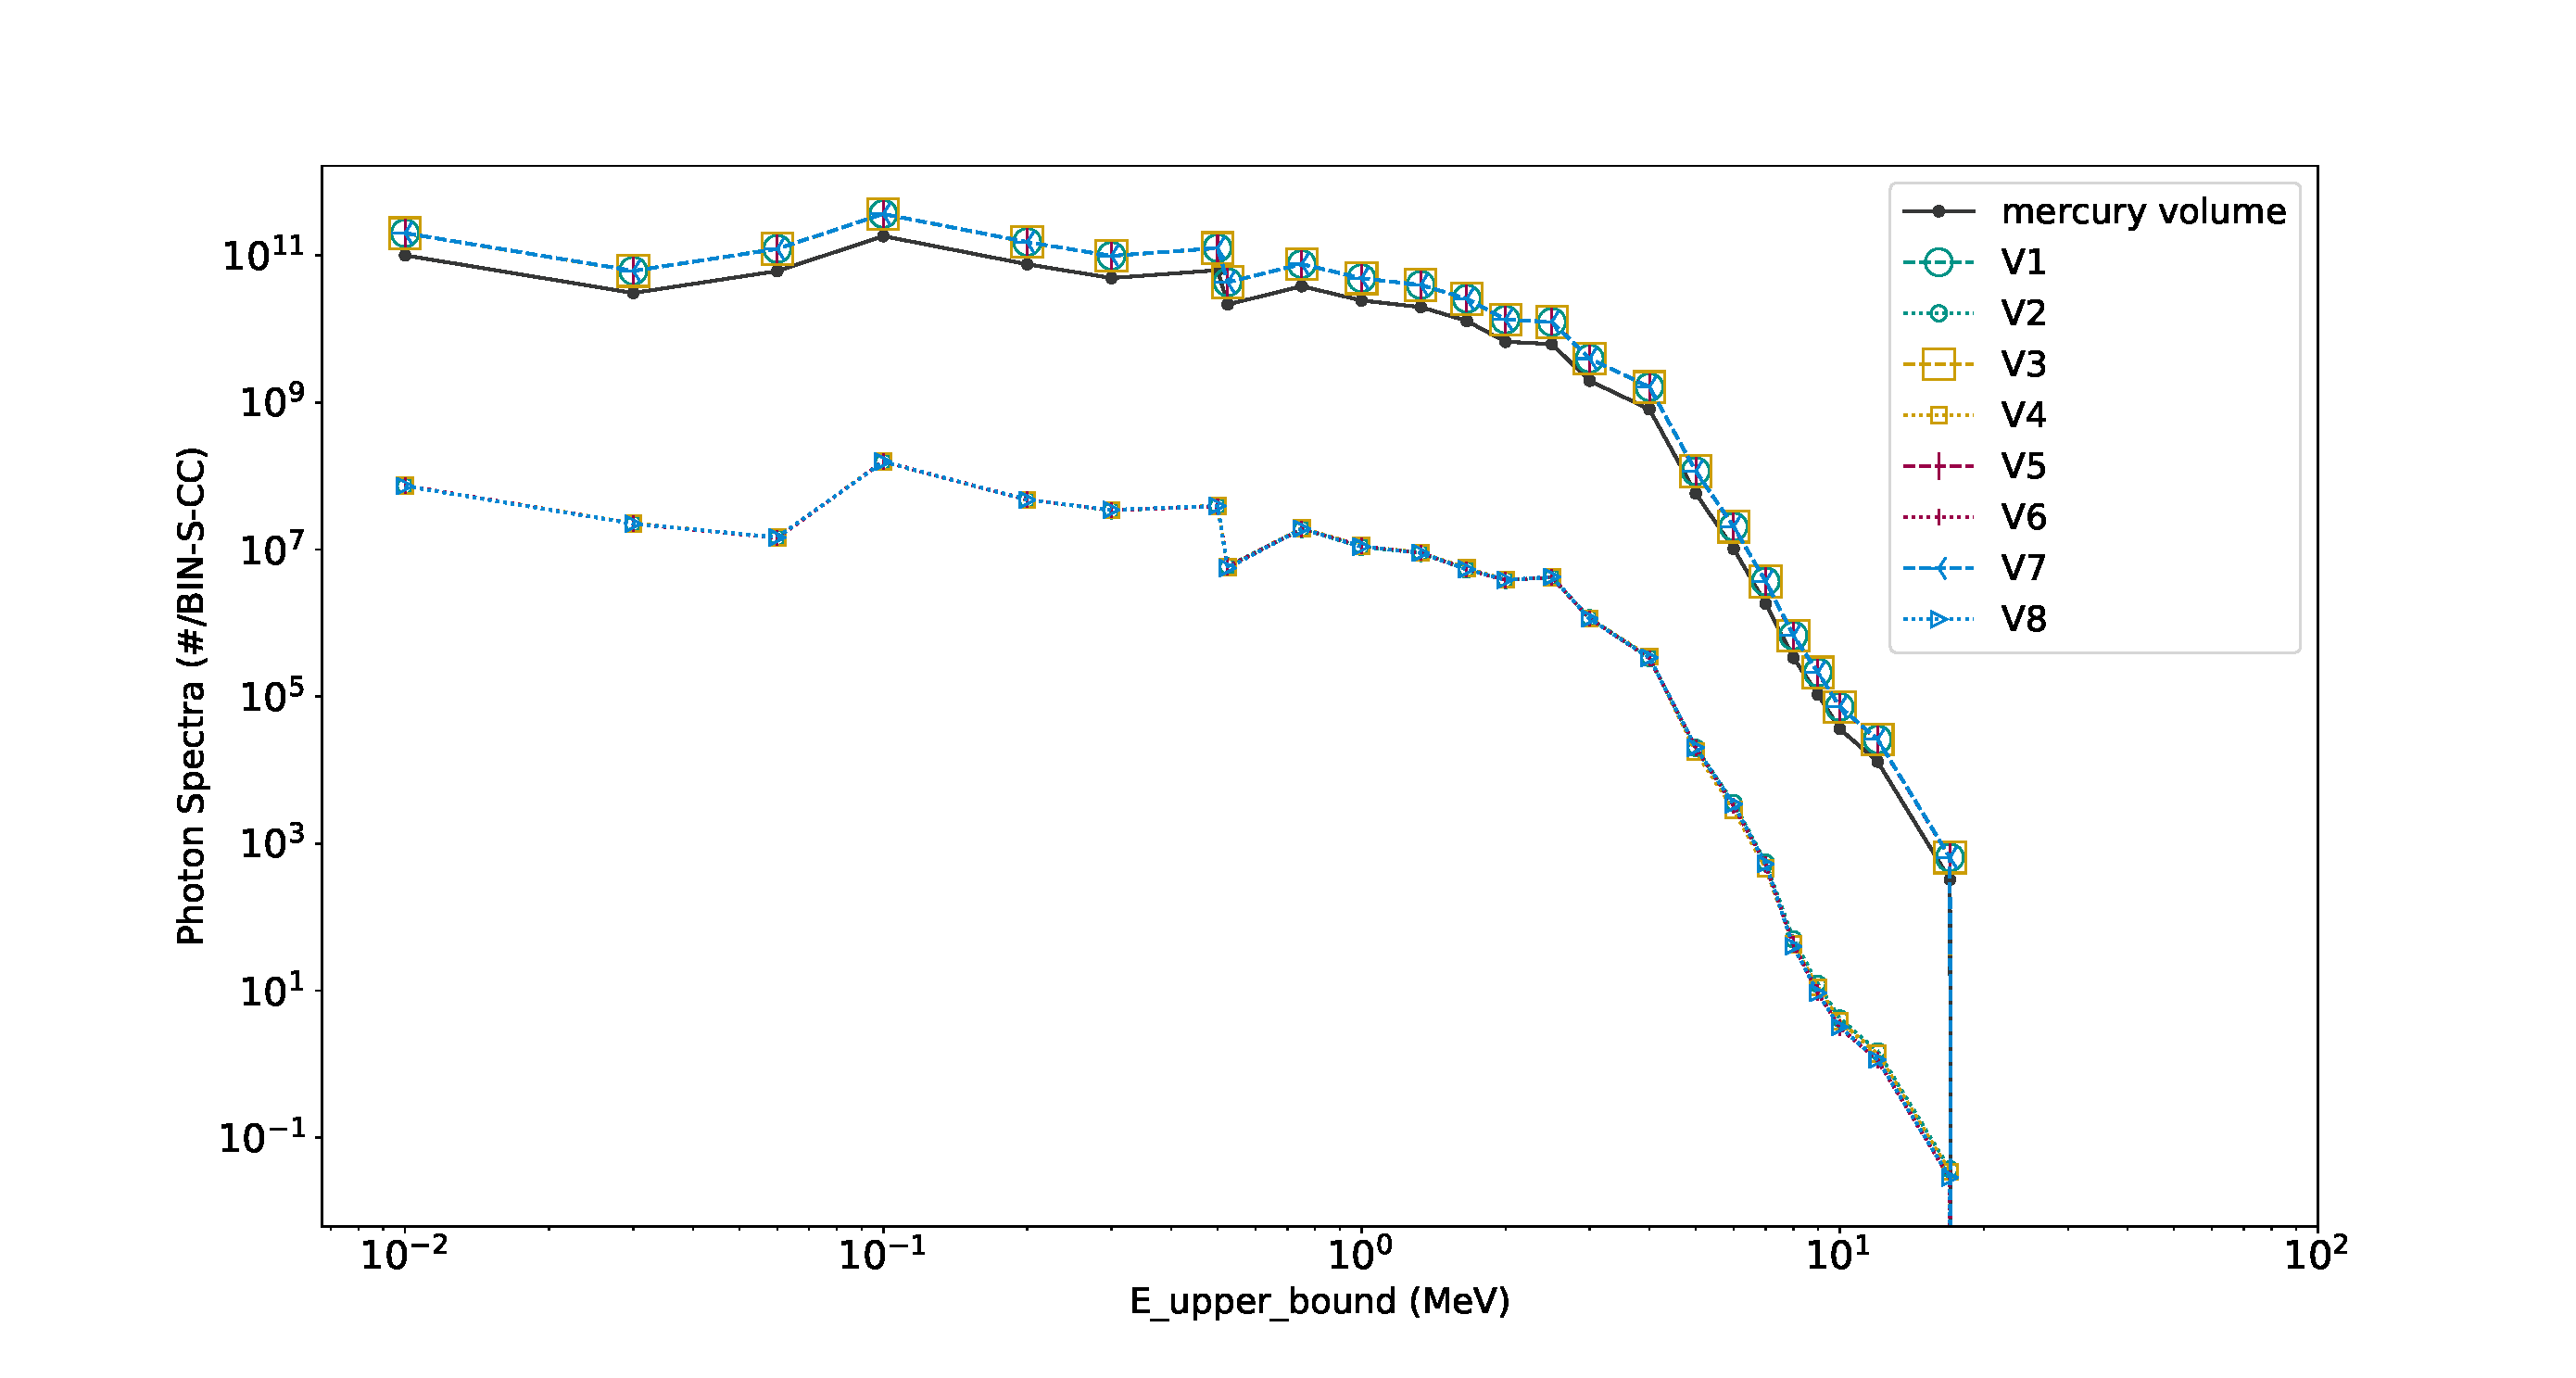
\includegraphics[scale=0.4, trim={2.5cm 1cm 3cm 3cm},clip]{../figs/toy_p1/spec_VPI_8.pdf}
	\end{subfigure}
	\caption{Photon emission density per voxel in a 2x2x2 mesh and the mercury cell}
	\label{fig:1spec_8v}
\end{figure}
%
The photon emission density served as a source for a photon transport. A perl
script was used to create a source card for \gls{mcnp}. This method was used
for the cell based workflow, so for the workflow using the full mercury cell,
and the divided geometry. For the problems with the superimposed mesh, a photon
emission density mesh was created to serve as the source.
Figure \ref{fig:1dose} show the biological doses using the sources created with
different methods. The left graphs are the results using the cell based
\gls{sdr}-rnucs workflow, and the on the right of the graph are the results
using the mesh \gls{sdr}-rnucs
workflow. As previously mentioned, the biological dose rate was collected in a
Cartesian mesh of same dimension for all problems.
\begin{figure}[H]
	\begin{subfigure}[t]{0.5\textwidth}
		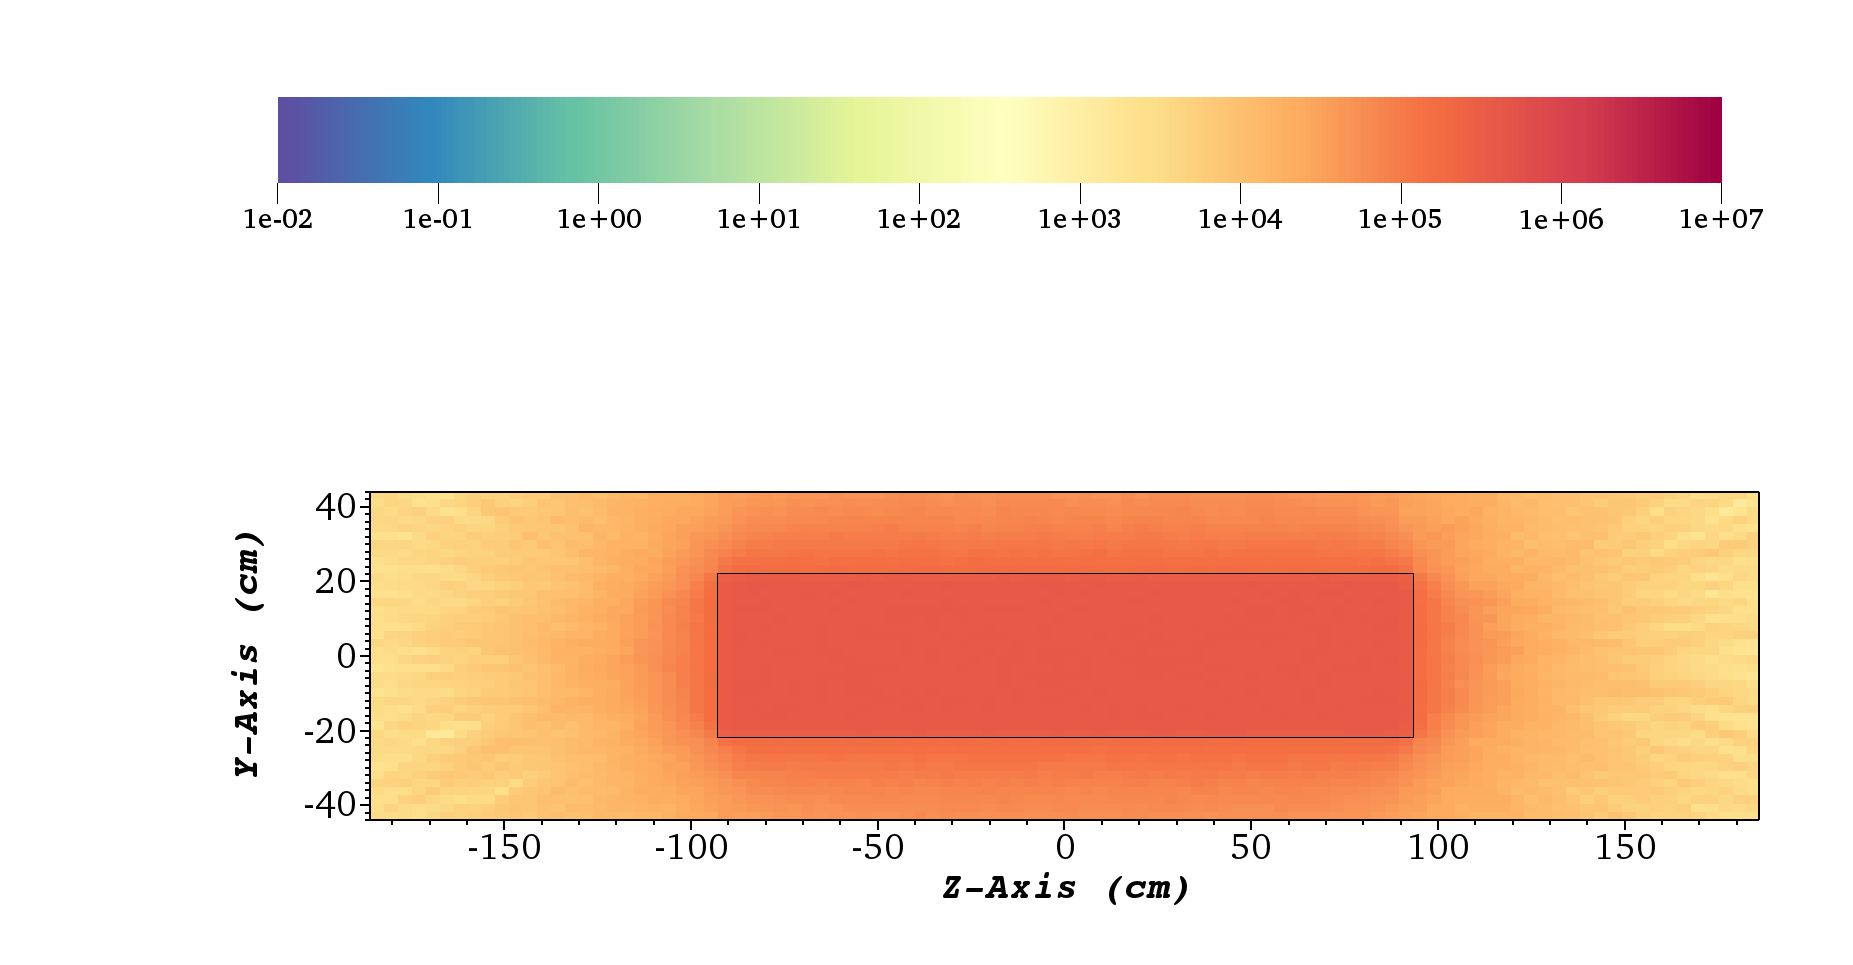
\includegraphics[width=\linewidth, trim={5cm 1cm 2cm 16cm},clip]{../figs/toy_p1/dose_VPI_original.png}
		\caption{full geometry}
		\label{fig:1dose_orig}
	\end{subfigure}\hfill
	\begin{subfigure}[t]{0.5\textwidth}
		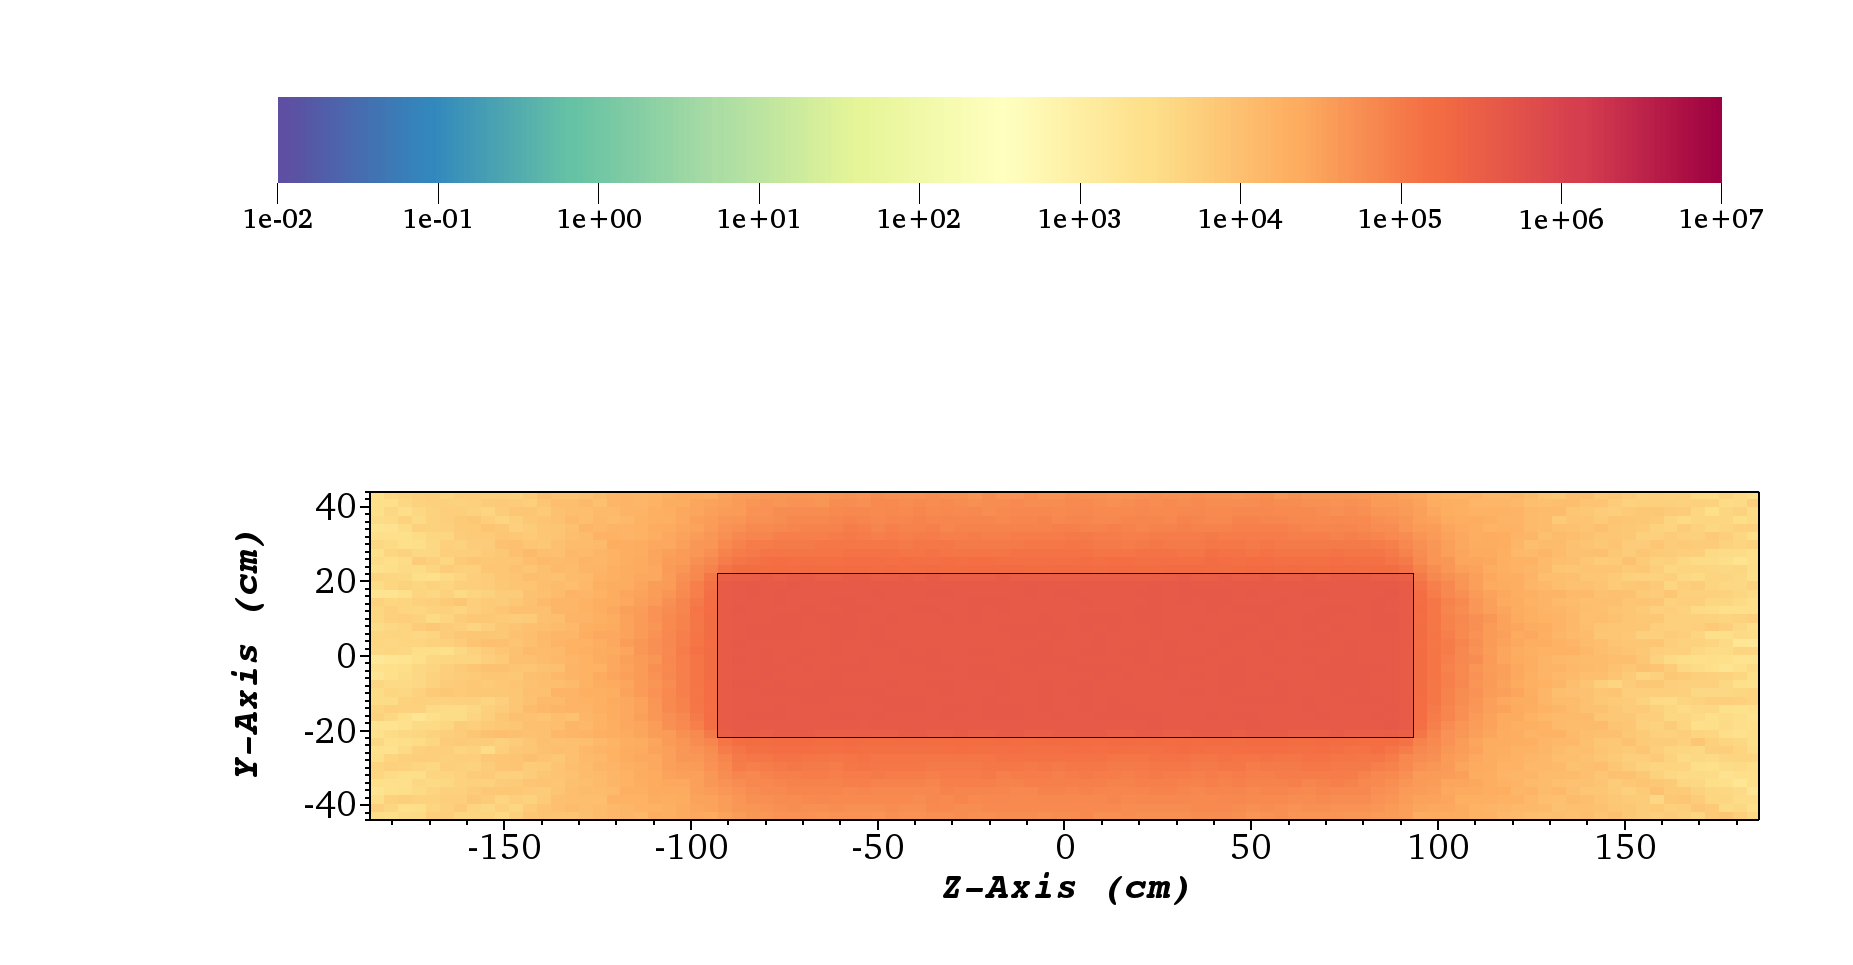
\includegraphics[width=\linewidth, trim={5cm 1cm 2cm 16cm},clip]{../figs/toy_p1/dose_VPI_1x_mesh.png}
		\caption{1x1x1 mesh}
		\label{fig:1dose_1x_mesh}
	\end{subfigure}

	\begin{subfigure}[t]{0.5\textwidth}
		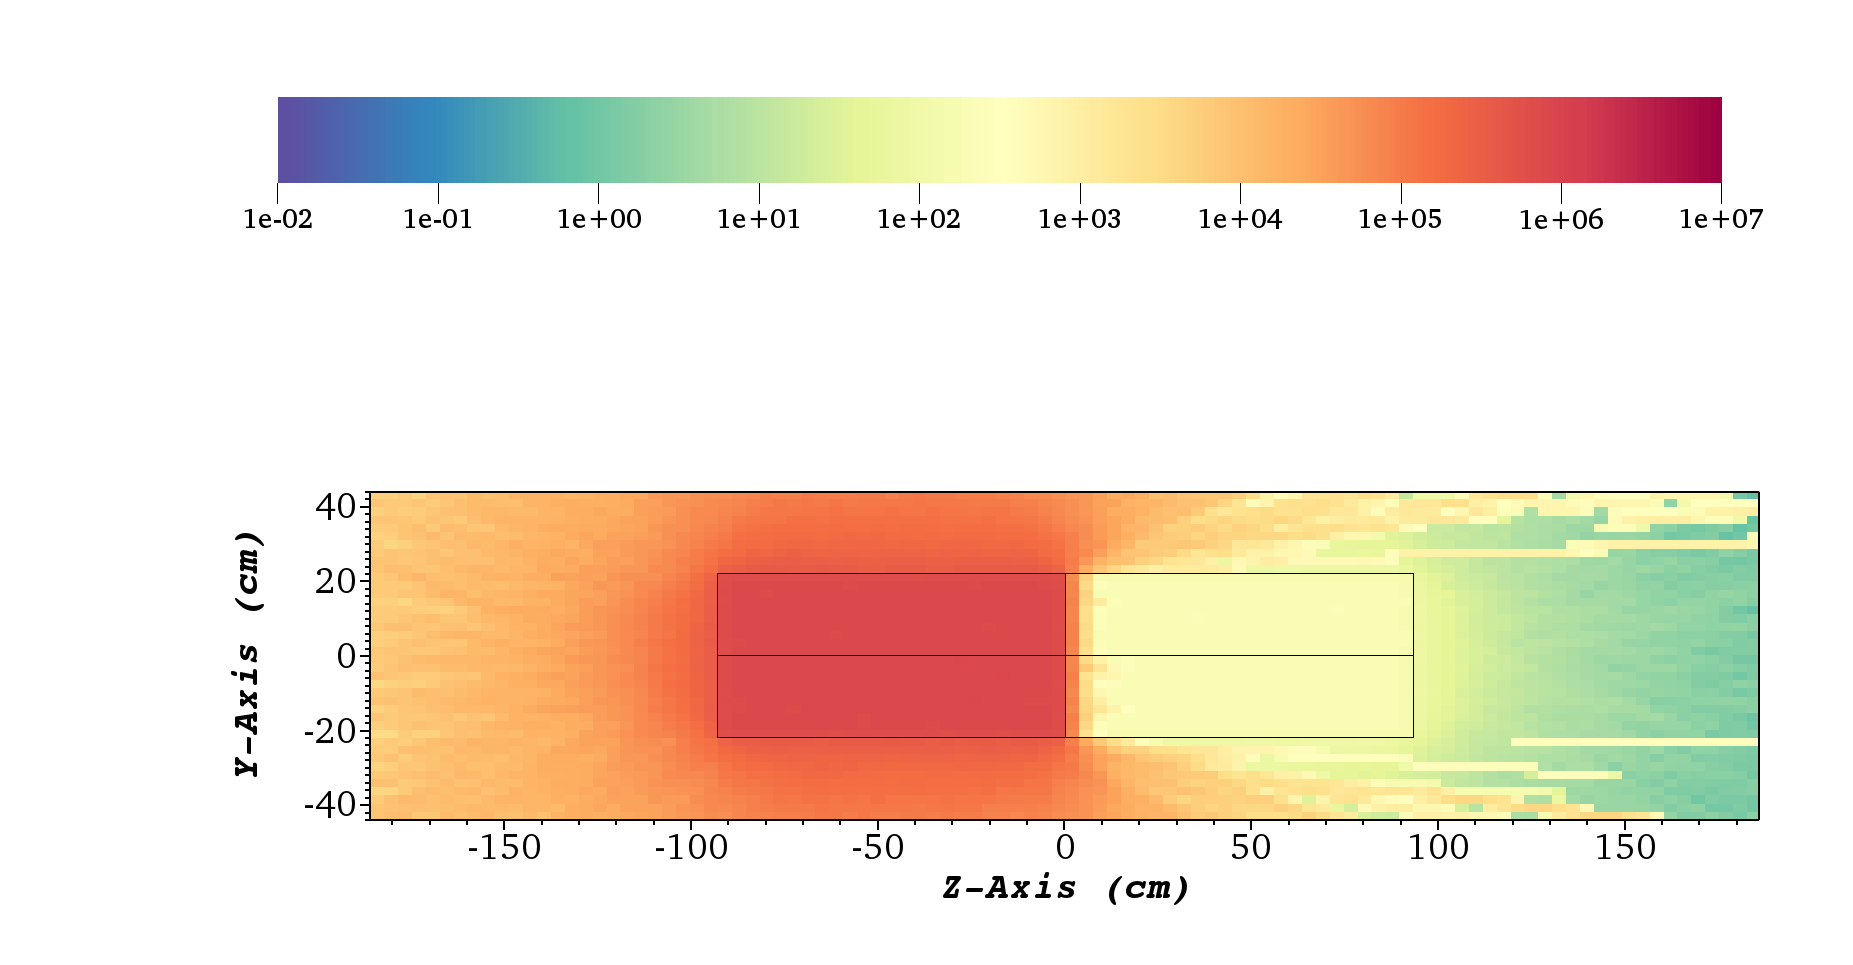
\includegraphics[width=\linewidth, trim={5cm 1cm 2cm 16cm},clip]{../figs/toy_p1/dose_VPI_2x_split.png}
		\caption{2x2x2 divided}
		\label{fig:1dose_2x_split}
	\end{subfigure}\hfill
	\begin{subfigure}[t]{0.5\textwidth}
		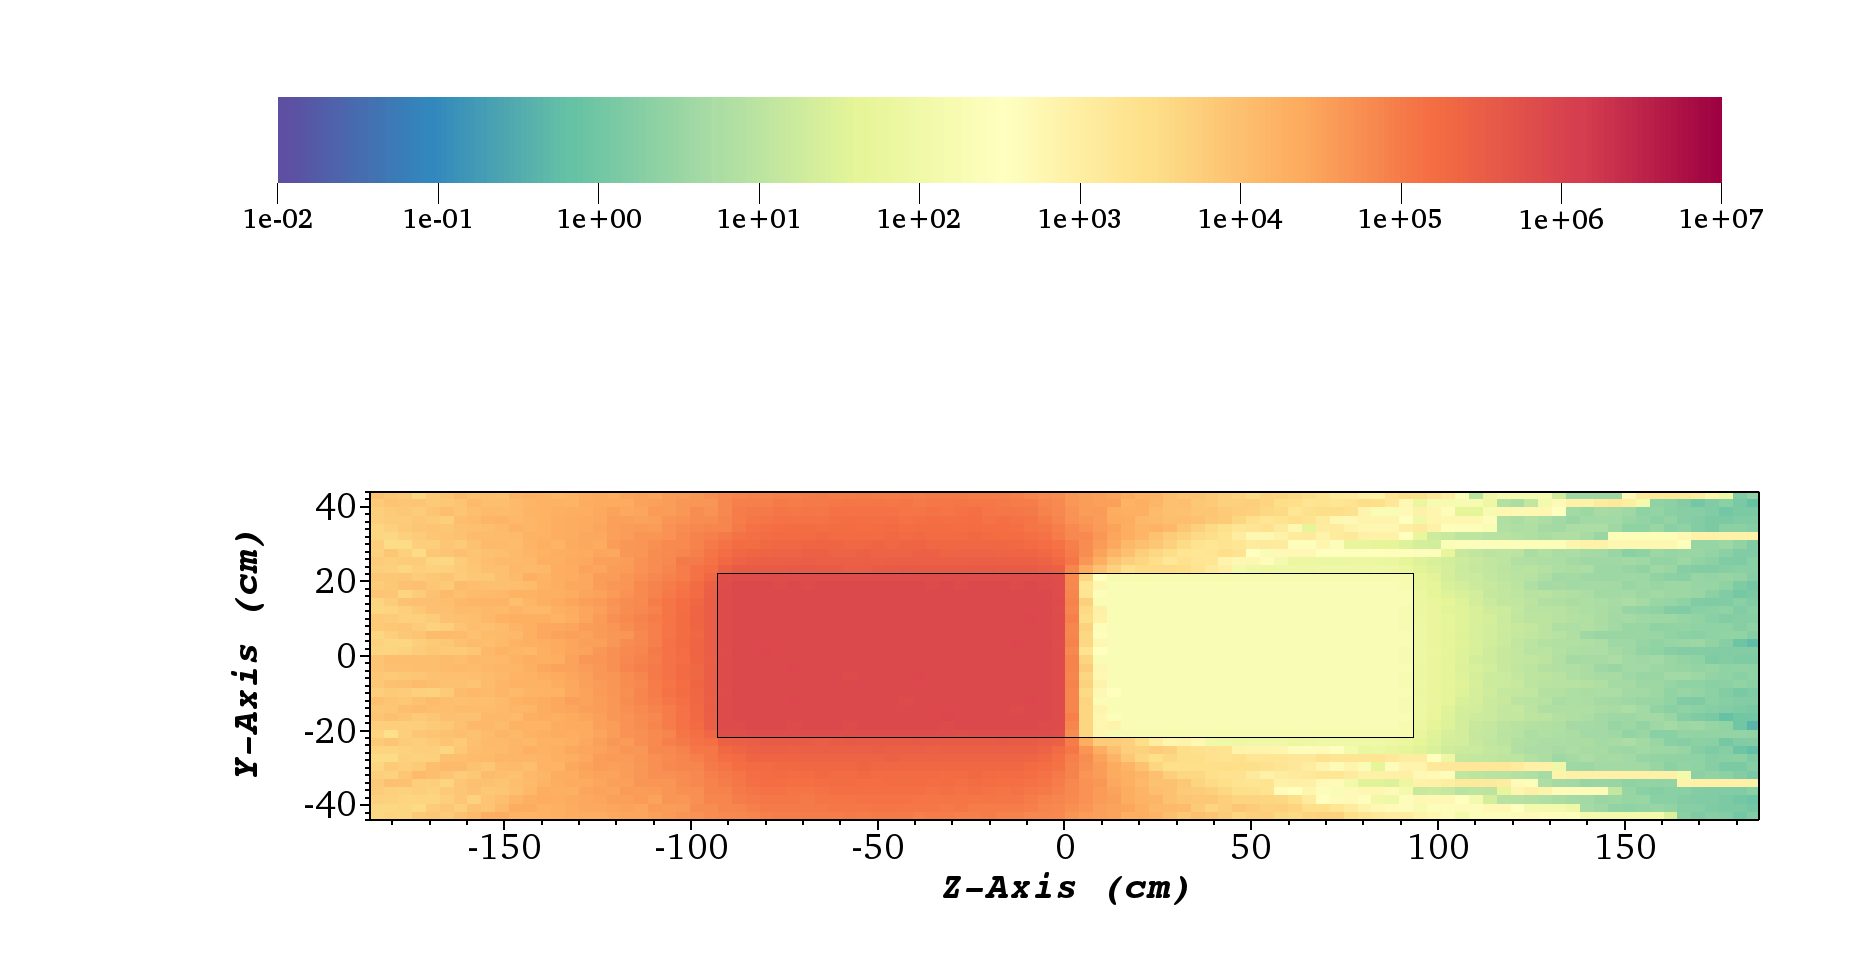
\includegraphics[width=\linewidth, trim={5cm 1cm 2cm 16cm},clip]{../figs/toy_p1/dose_VPI_2x_mesh.png}
		\caption{2x2x2 mesh}
		\label{fig:1dose_2x_mesh}
	\end{subfigure}

	\begin{subfigure}[t]{0.5\textwidth}
		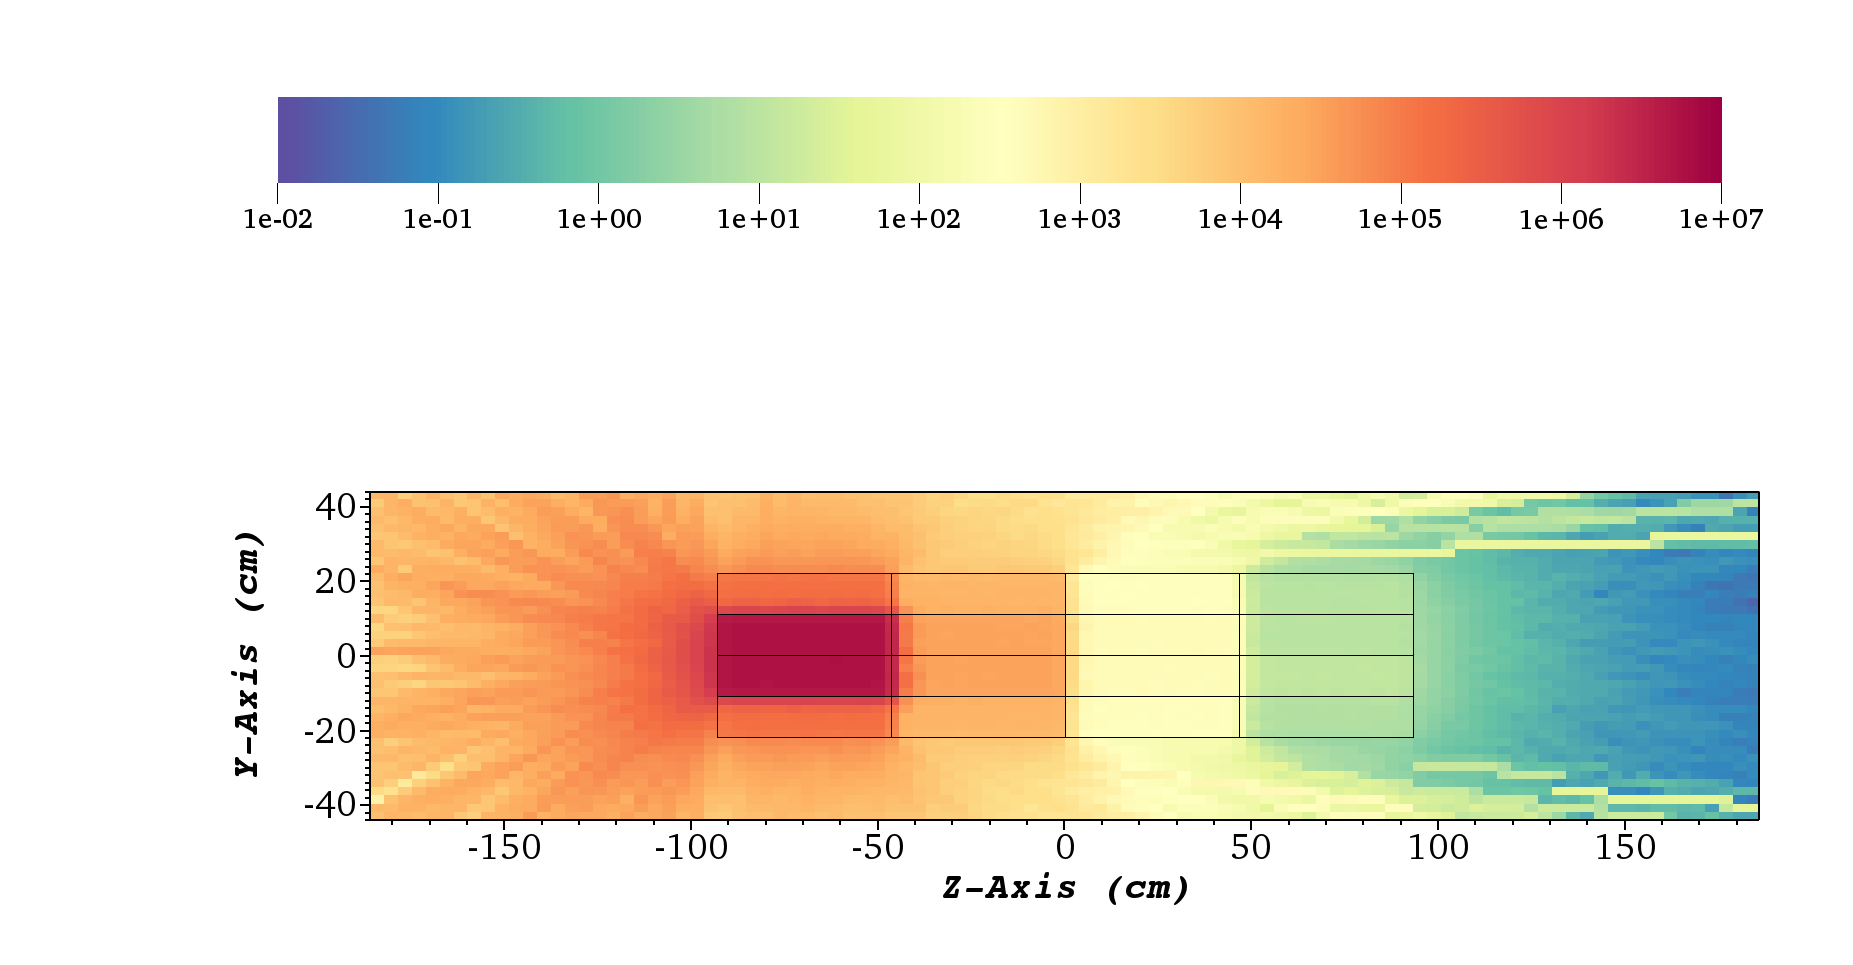
\includegraphics[width=\linewidth, trim={5cm 1cm 2cm 16cm},clip]{../figs/toy_p1/dose_VPI_4x_split.png}
		\caption{4x4x4 divided}
		\label{fig:1dose_4x_split}
	\end{subfigure}\hfill
	\begin{subfigure}[t]{0.5\textwidth}
		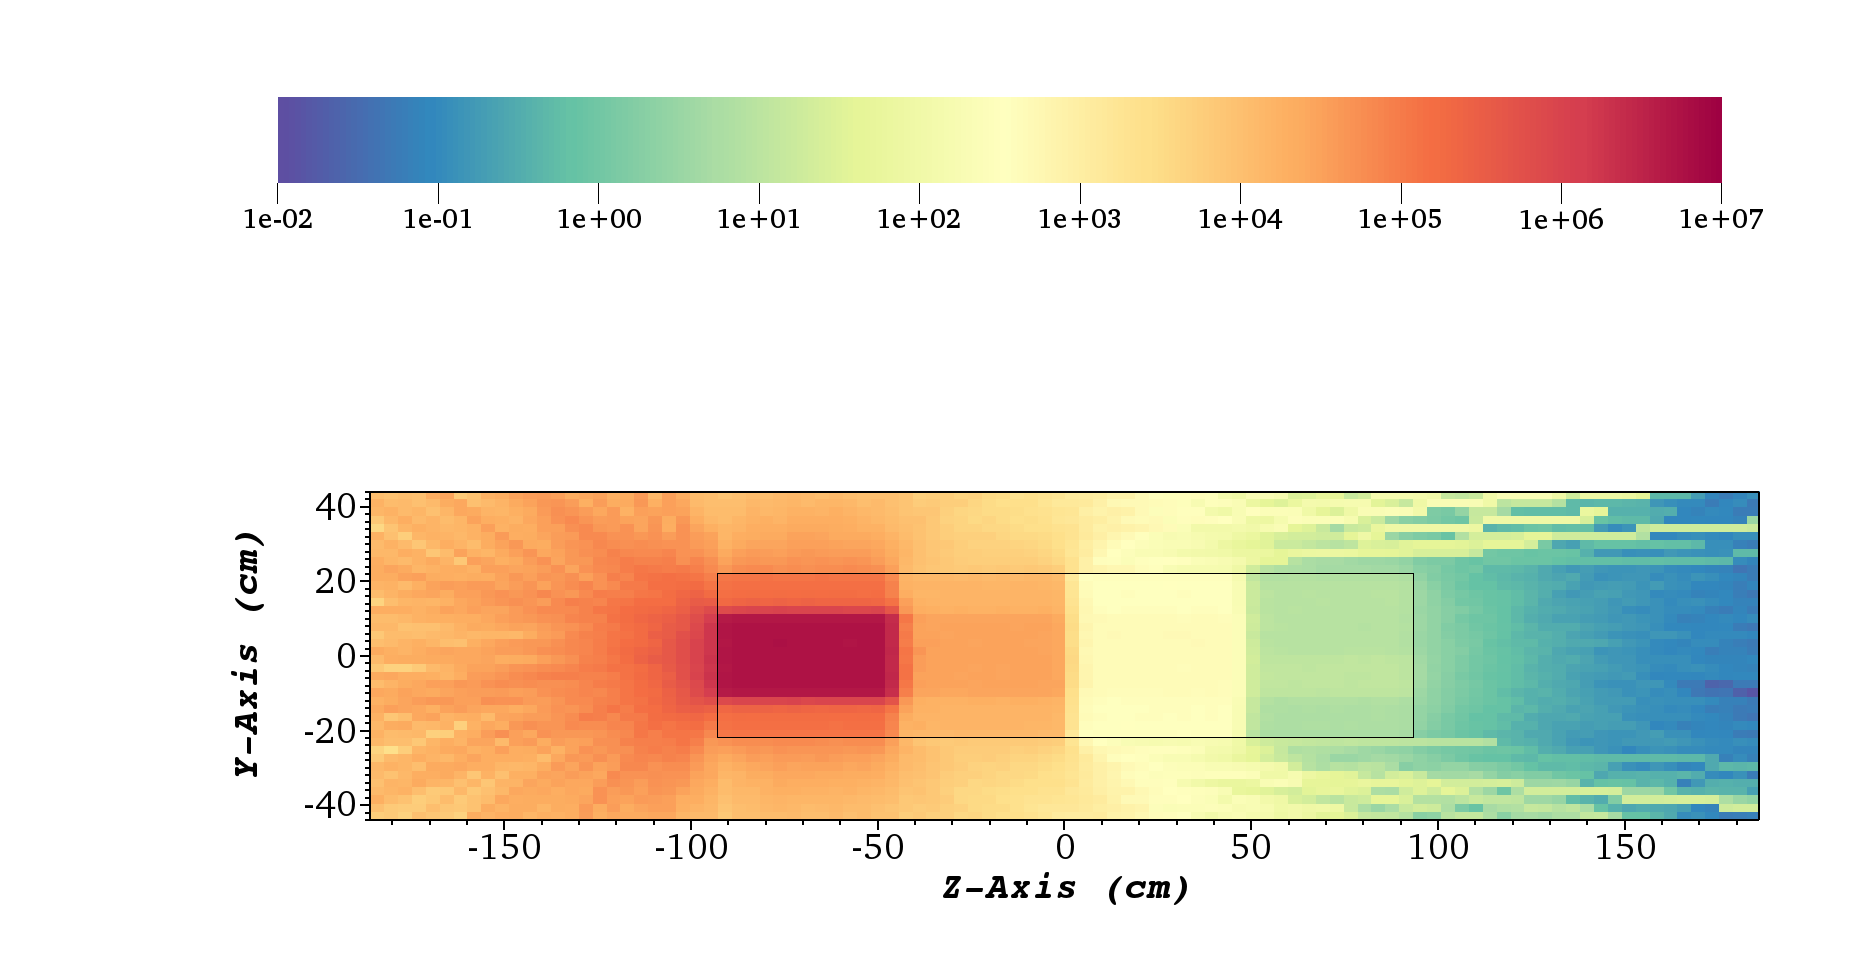
\includegraphics[width=\linewidth, trim={5cm 1cm 2cm 16cm},clip]{../figs/toy_p1/dose_VPI_4x_mesh.png}
		\caption{4x4x4 mesh}
		\label{fig:1dose_4x_mesh}
	\end{subfigure}

	\begin{subfigure}[t]{1.0\textwidth}
		\centering
		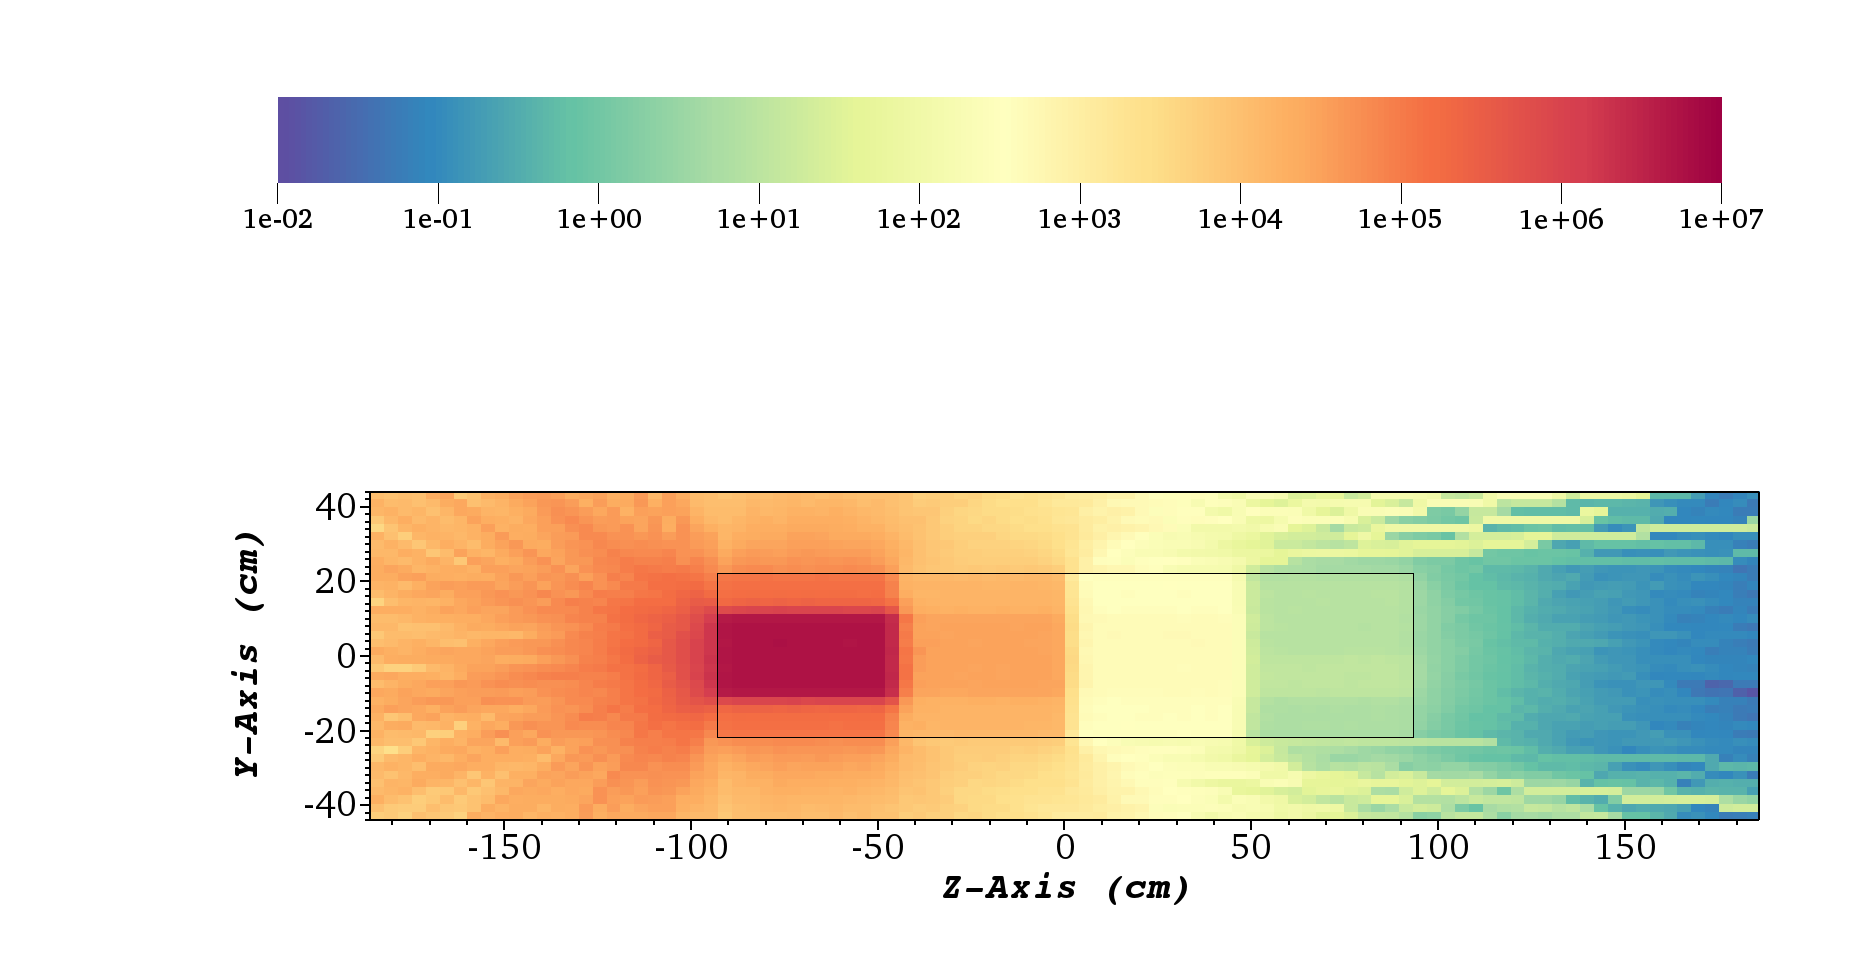
\includegraphics[width=\linewidth, trim={5cm 25cm 2cm 2cm},clip]{../figs/toy_p1/dose_VPI_4x_mesh.png}
		\label{fig:1legend}
	\end{subfigure}
	\caption{Biological dose rate on the mercury cell with mesh and divided geometry}
	\label{fig:1dose}
\end{figure}
%
In order to assess the differences across the two methods, a z-score test was
performed. Figure \ref{fig:1zscores} shows the \gls{pdf} and \gls{cdf} of a
z-sore test comparing the biological dose rates per voxel obtained using a
cell based source and the ones obtained using a mesh based source. The results
of the mesh based source are compared to their corresponding cell based source
results.
\begin{figure}[H]
	\begin{subfigure}[h]{1.0\textwidth}
		\centering
		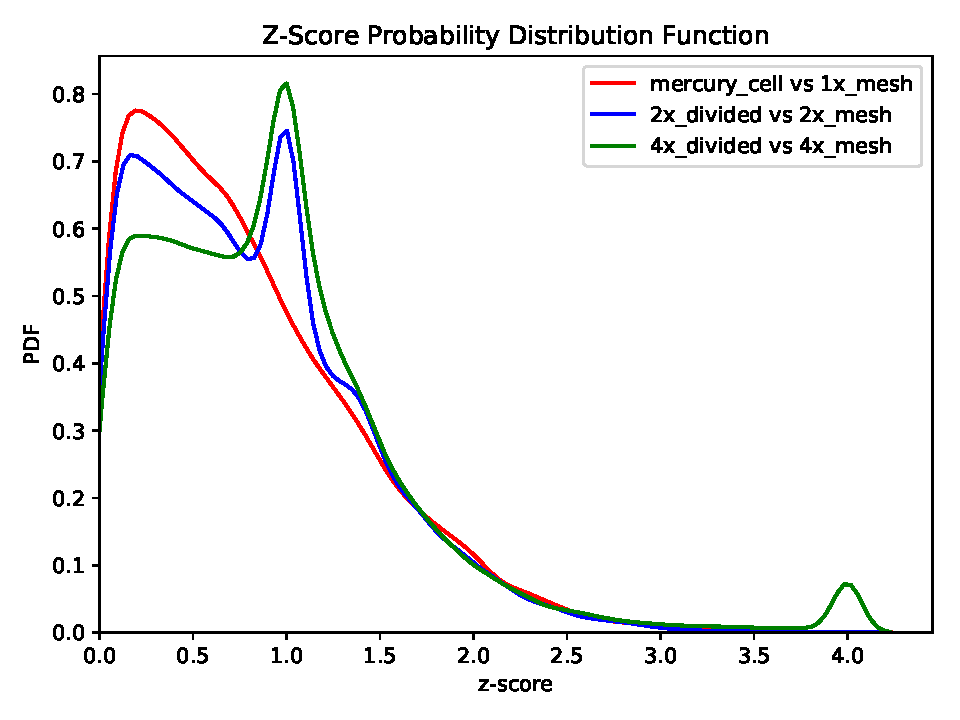
\includegraphics[scale=0.85, trim={0cm 0cm 0cm 0.9cm},clip]{../figs/toy_p1/PDF_zscore_VPI_all.pdf}
		\caption{Probability Distribution Function}
		\label{fig:1VPI_pdf}
	\end{subfigure}
	\hfill
	\begin{subfigure}[h]{1.0\textwidth}
		\centering
		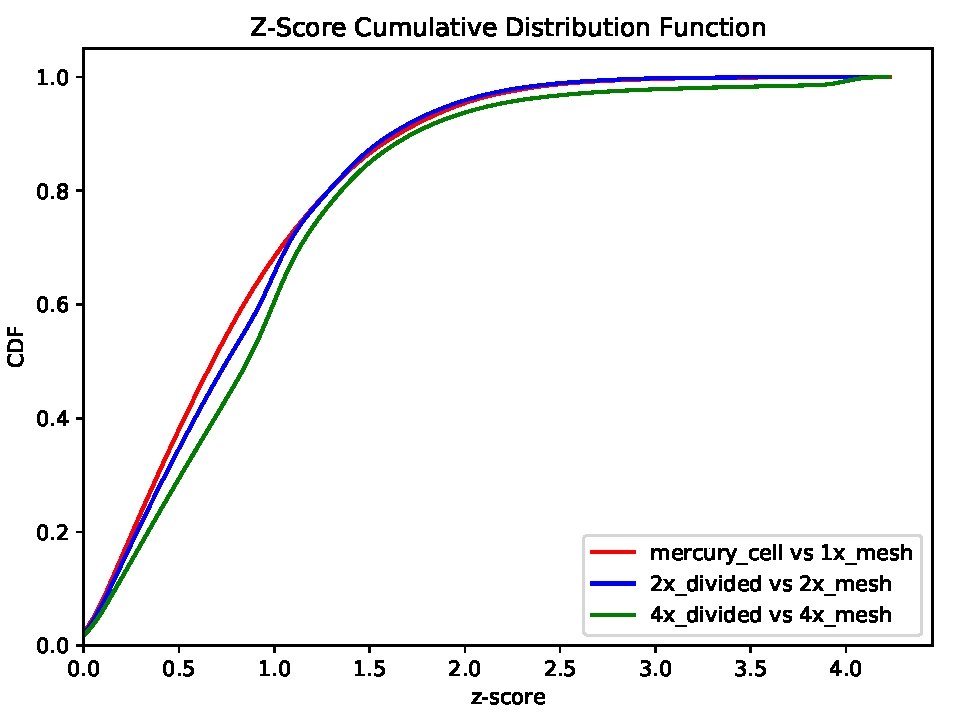
\includegraphics[scale=0.85, trim={0cm 0cm 0cm 0.8cm},clip]{../figs/toy_p1/CDF_zscore_VPI_all.pdf}
		\caption{Cumulative Distribution Function}
		\label{fig:1VPI_cdf}
	\end{subfigure}
	\caption{PDF and CDF of the z-value of each mesh voxel when comparing the cell workflow to the mesh workflow}
	\label{fig:1zscores}
\end{figure}

%%%%%%%%%%%%%%%%%%

\newpage

\subsubsection{Verification Problem II}
Similar analysis were done for the second verification problem. Figure
\ref{fig:2prod_cell_1x_2x_4x} shows the combined isotope production collected
in the mercury and steel volumes, and the isotope production combined for all
voxels in each of the meshes. The bottom graph shows the relative change when
comparing each of the meshes to the isotope production collected in both cells.
The relative change between the isotope production collected in a mesh compared
to the one collected in the cell are mostly within statistic agreement. There
some isotopes that are different.
%
\begin{figure}[H]
 \centering
 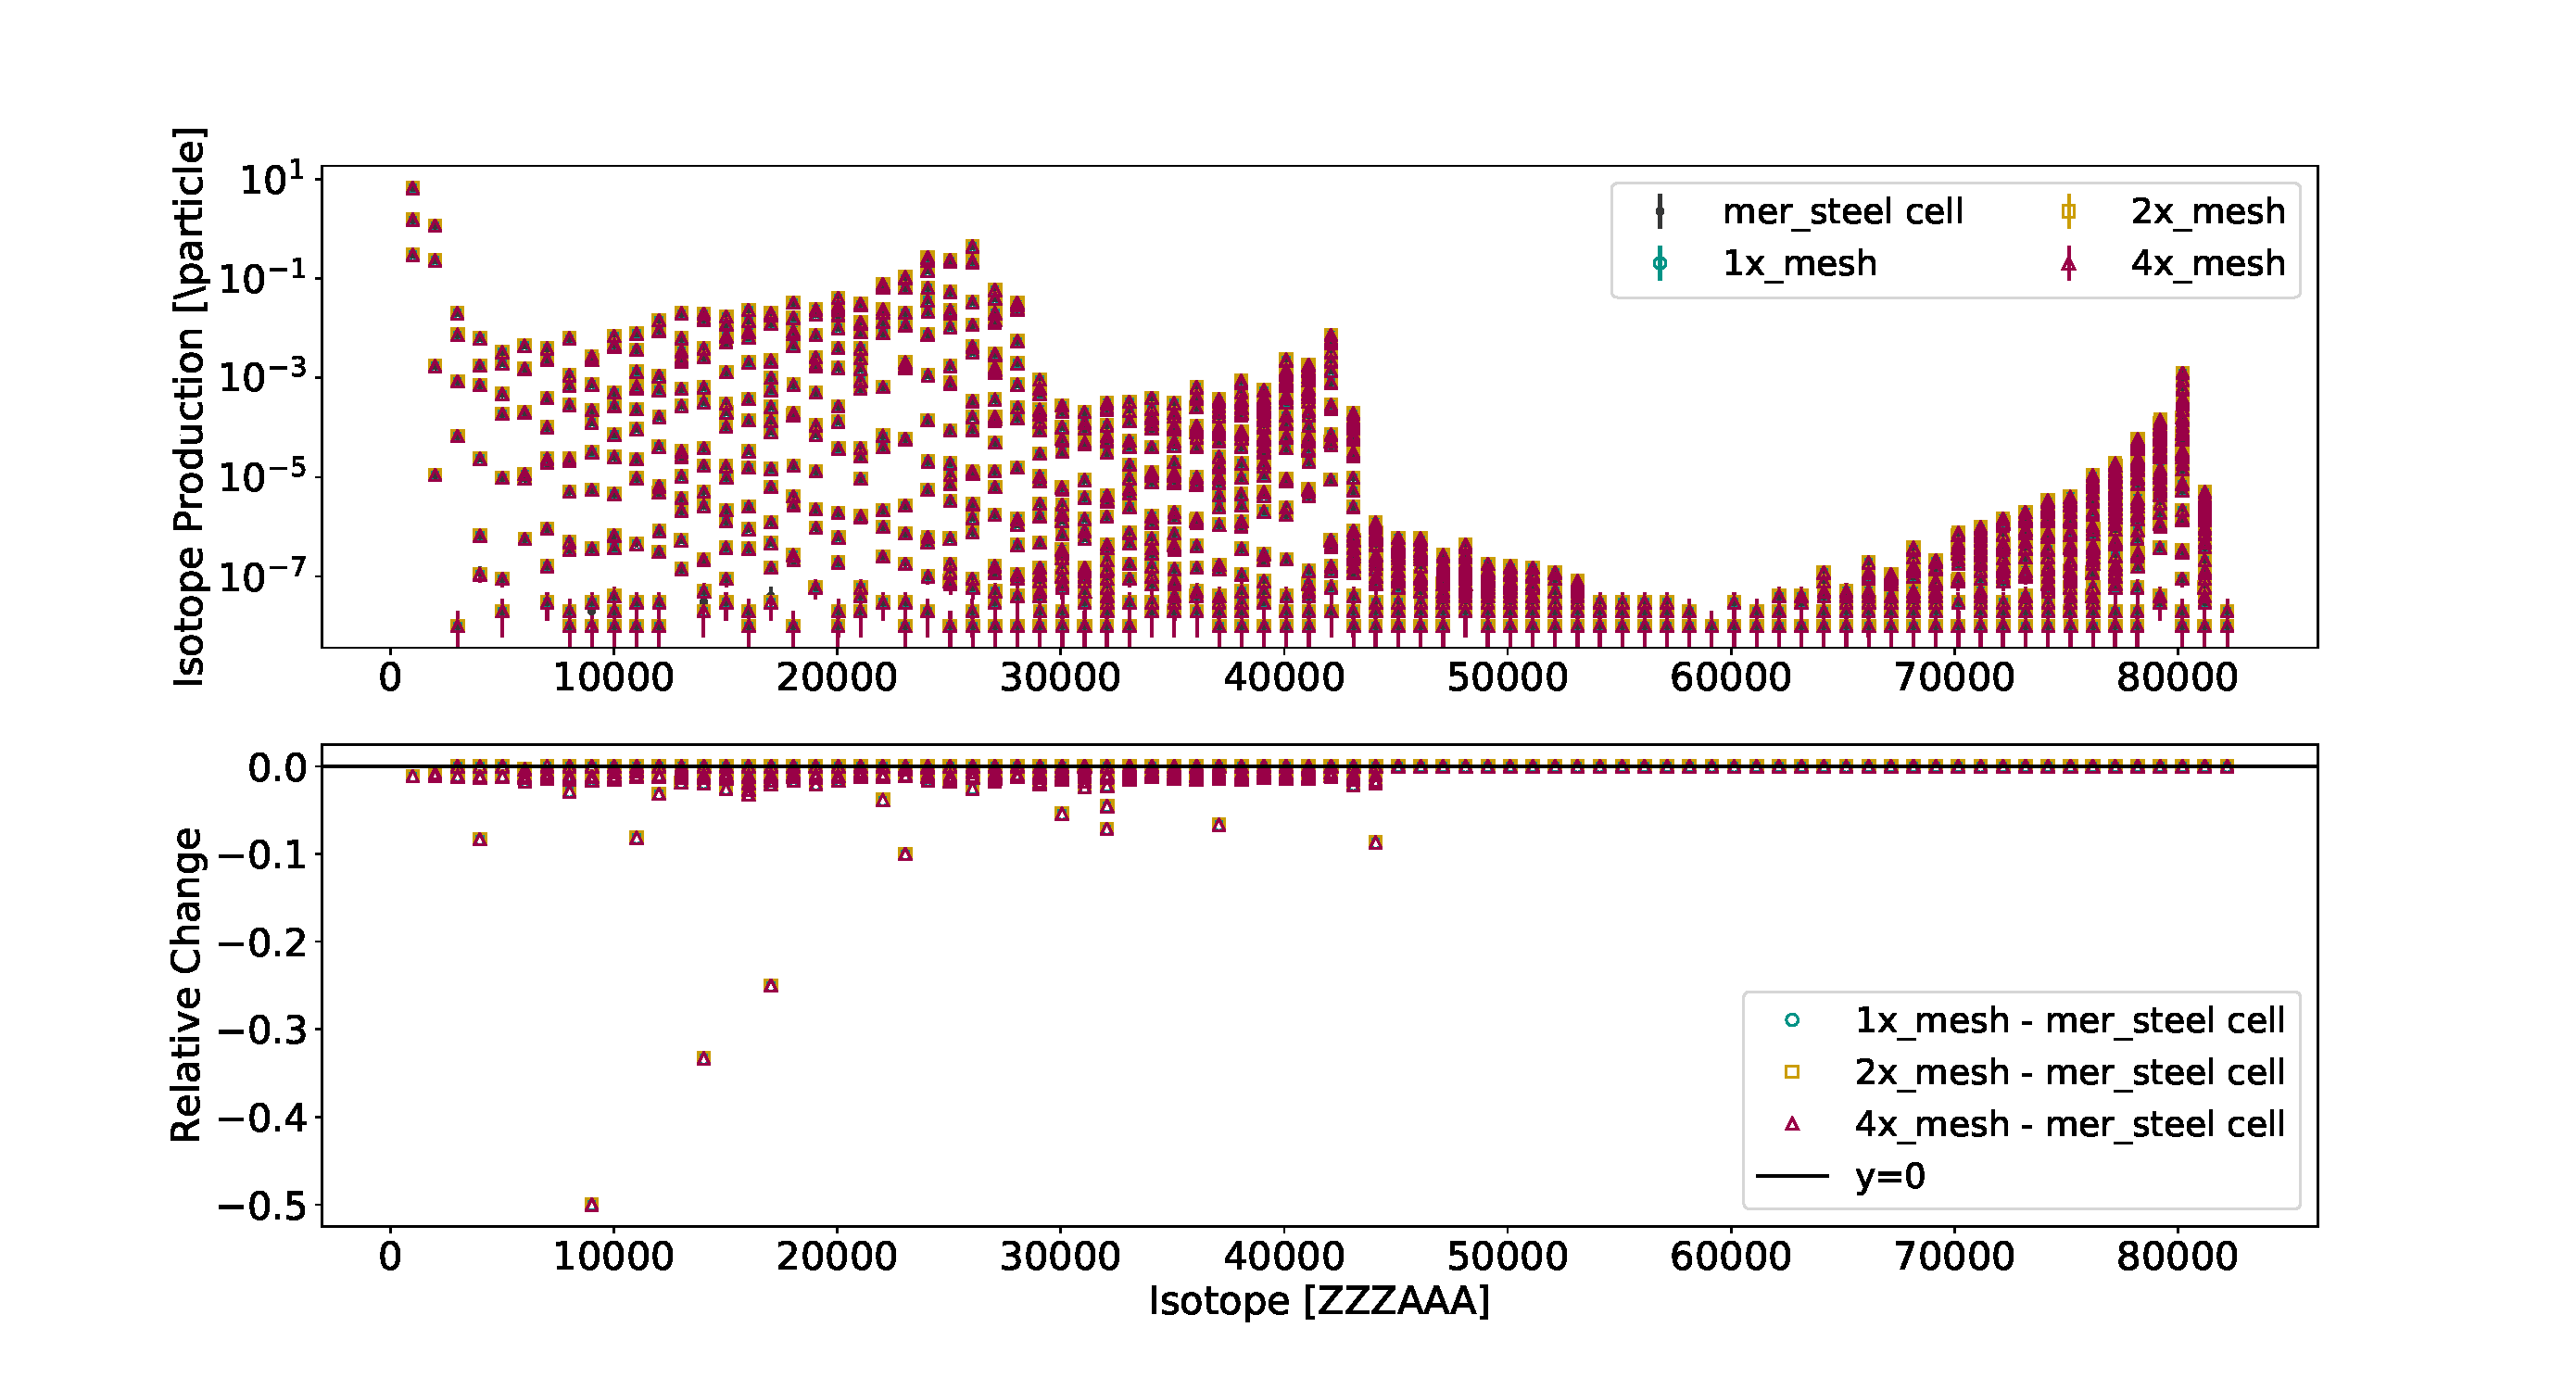
\includegraphics[scale=0.4,trim={2cm 1cm 3cm 2cm},clip]{../figs/toy_p2/prod_VPII_1x_2x_4x.pdf}
 \caption{Radionuclide production for mercury/steel cells and Cartesian meshes}
 \label{fig:2prod_cell_1x_2x_4x}
\end{figure}
%
Figure \ref{fig:2prod_cell_2x} compares the isotope production collected in the
mercury and steel volumes to the summed up results of a 2x2x2 mesh and the 2x2x2
divided geometry. In this case, one can see great differences in the divided
geometry. This is likely due to having to mix materials during the
neutron/proton transport for the divided geometry while the original problem
and the mesh did not have to mix materials in this step.
Figure \ref{fig:2prod_cell_2x_r} show the relative difference between the
divided geometry and the original problem, as well as the relative difference
between the mesh and the original problem. Both as functions of the isotope
production results obtained in the mercury and steel volume.
%
\begin{figure}[H]
 \centering
 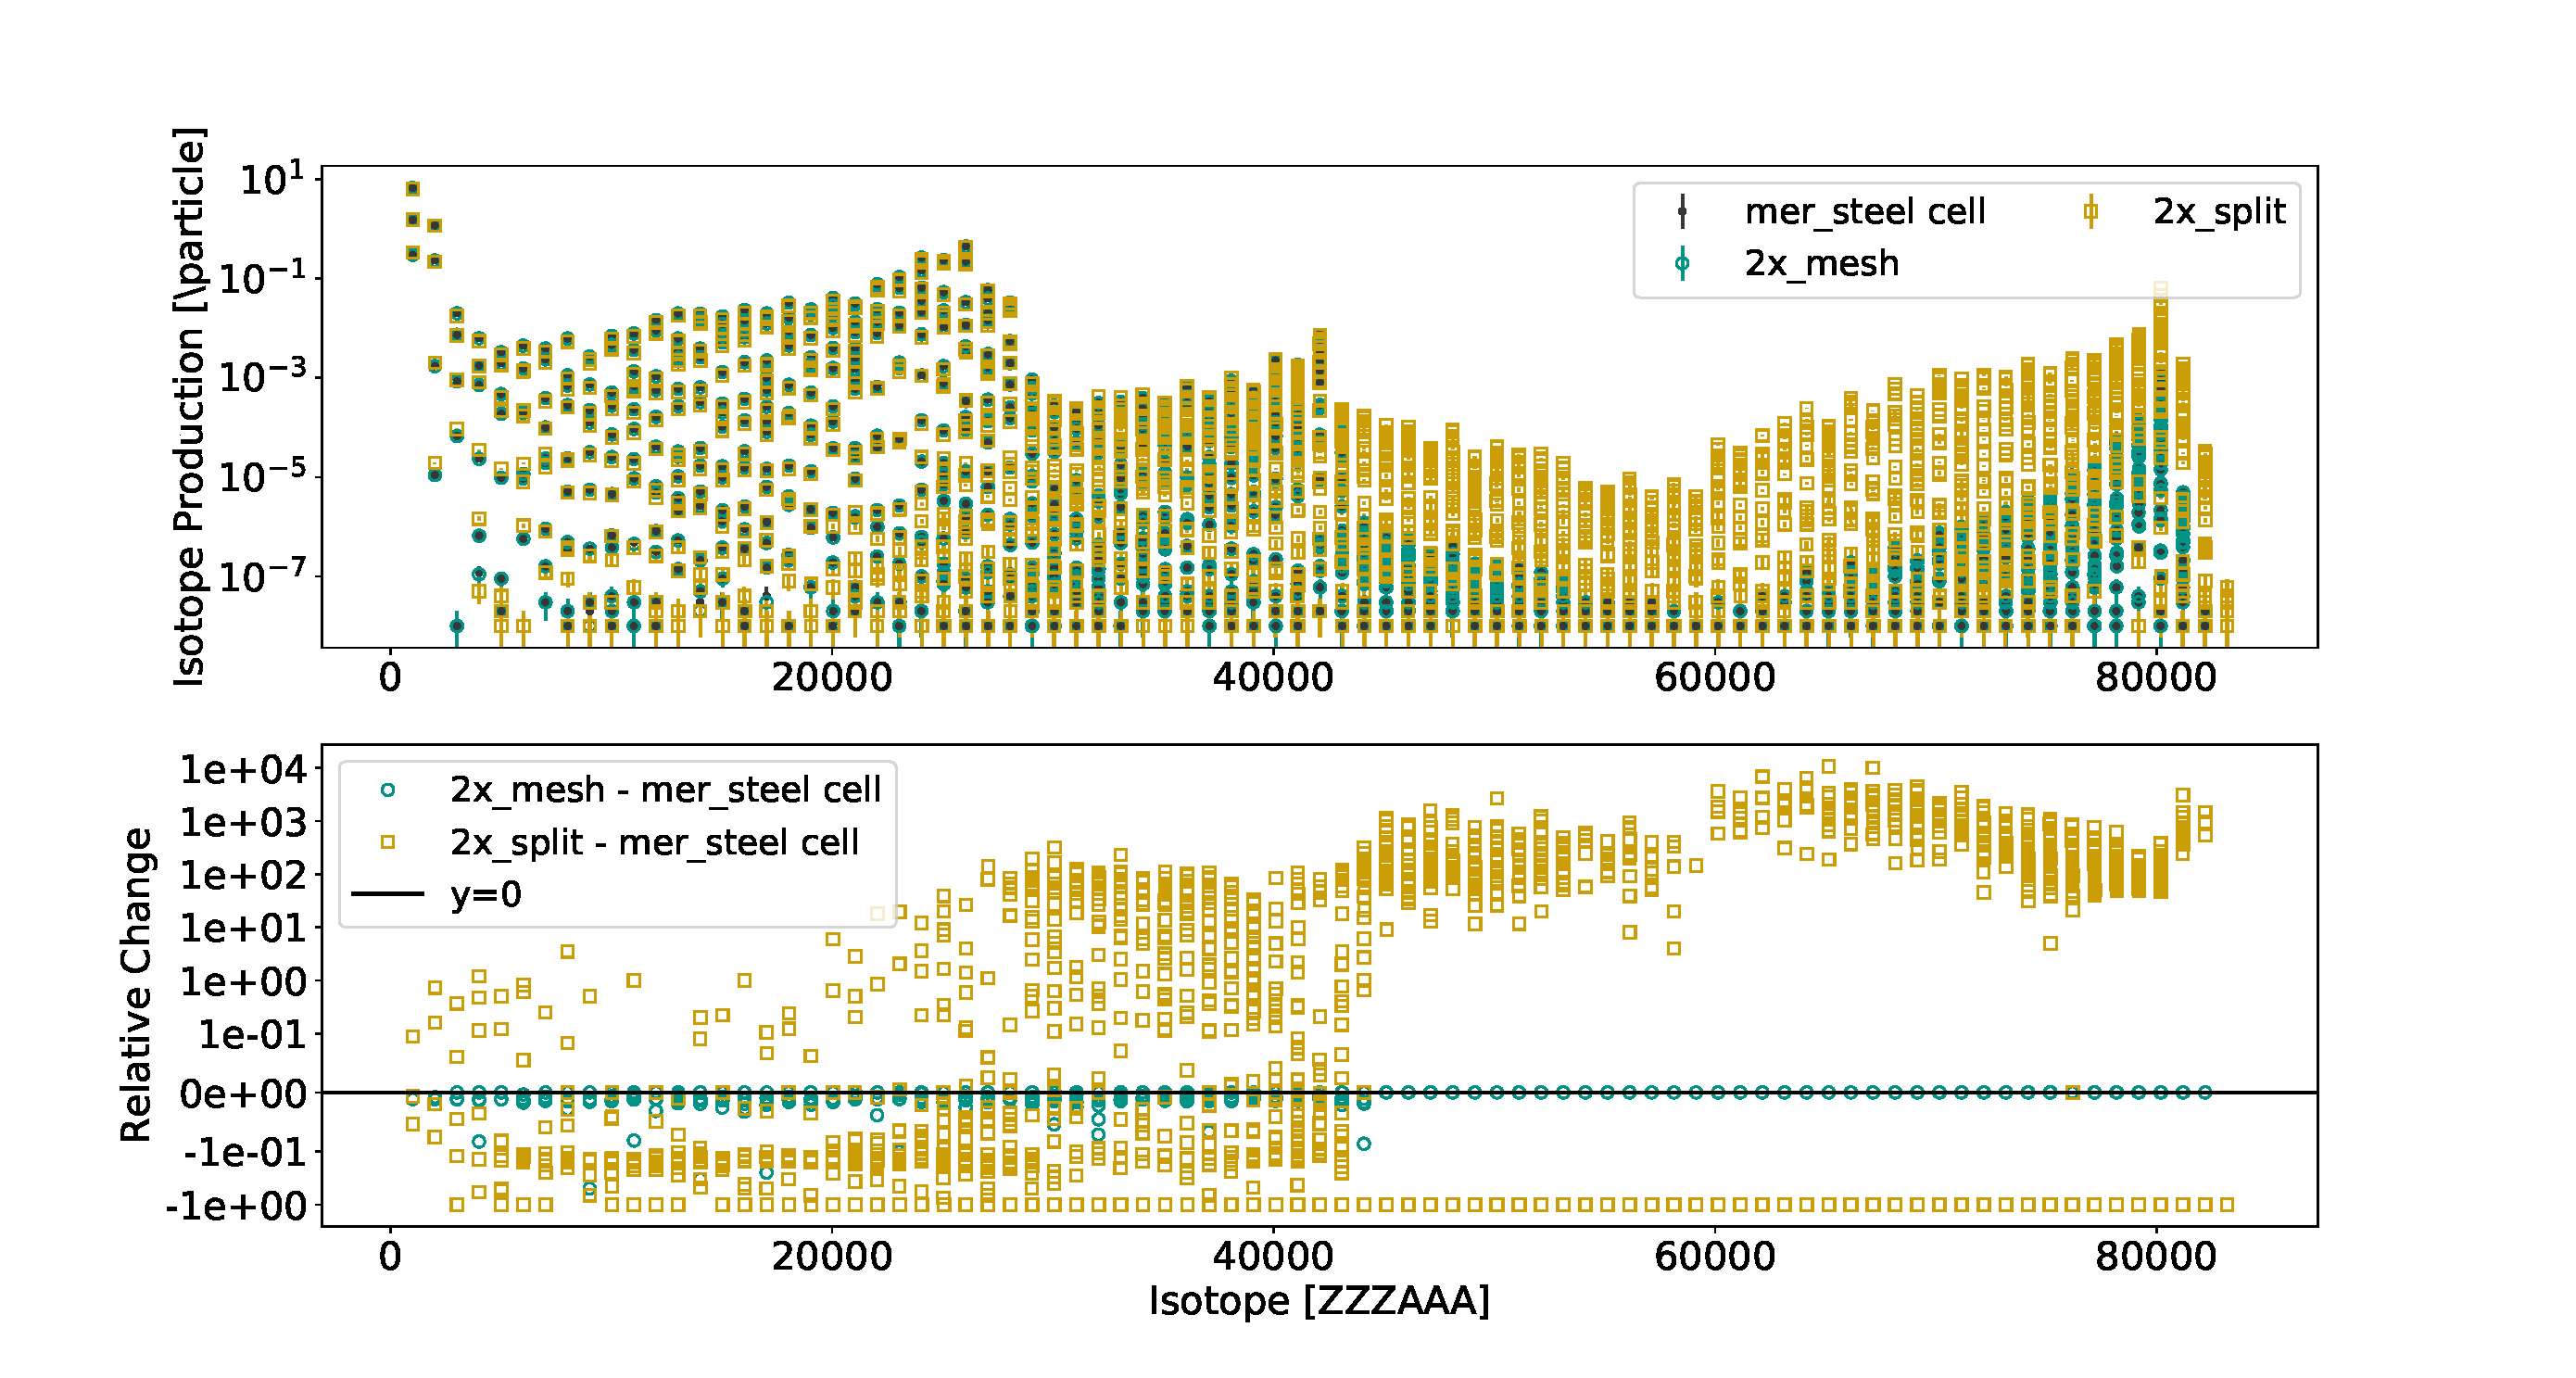
\includegraphics[scale=0.4,trim={2cm 1cm 3cm 2cm},clip]{../figs/toy_p2/prod_VPII_2x.pdf}
 \caption{Radionuclide production mercury/steel cells, 2x2x2 mesh, and 2x2x2 divided geometry}
 \label{fig:2prod_cell_2x}
\end{figure}
%
\begin{figure}[H]
 \centering
 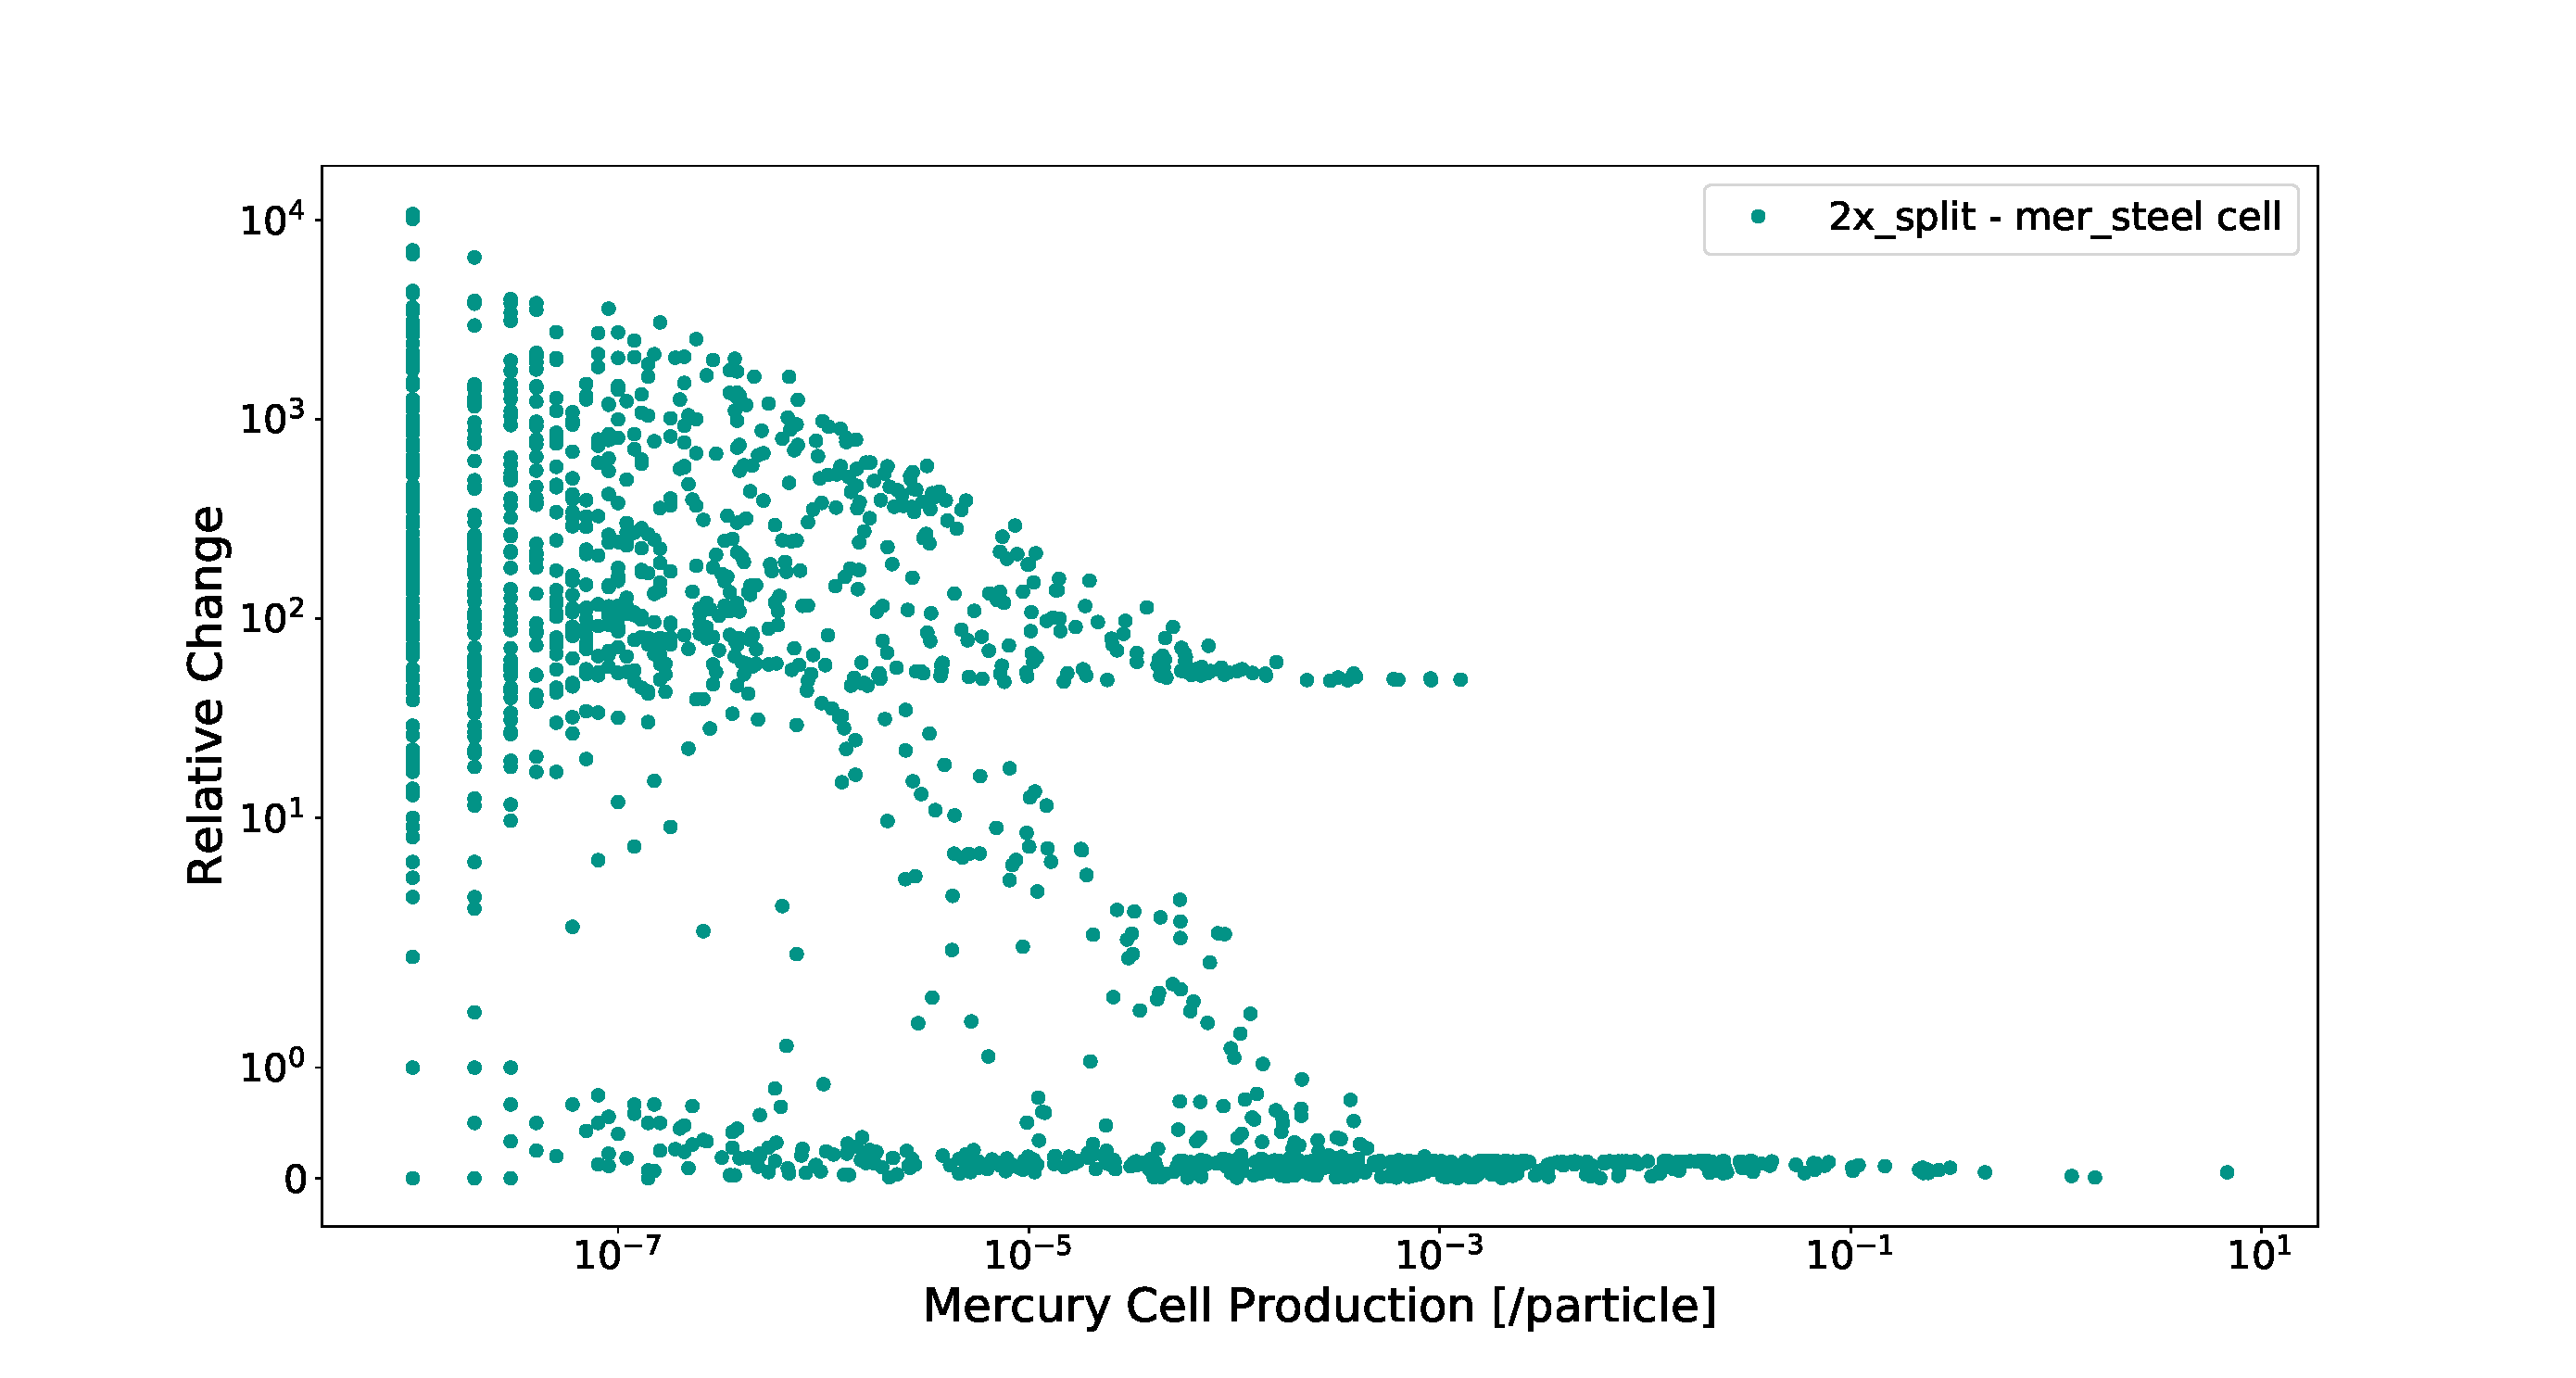
\includegraphics[scale=0.35,trim={3cm 0.5cm 4.5cm 3cm},clip]{../figs/toy_p2/prod_VPII_rc_2x_split.pdf}
 \caption{Relative change between cell method and 2x2x2 geometry split vs. the isotope production of the mercury cell}
 \label{fig:2prod_cell_2x_rc}
\end{figure}
%
Figure \ref{fig:2prod_cell_4x} shows a similar comparing as Figure
\ref{fig:2prod_cell_2x} but for the 4x4x4 mesh and the 4x4x4 divided geometry.
The behavior of the relative change seen at the bottom of the graph is similar
to the behavior seem in a similar analysis done for the first problem.
A graph comparing the relative change between the results collected in the
divided geometry, and in the mercury and steel volumes, as well as the relative
difference between the information collected in the 4x4x4 mesh and the
information collected in the mercury and steel cell. Both as a function of the
the isotope production results obtained in the mercury and steel volume.
%
\begin{figure}[H]
 \centering
 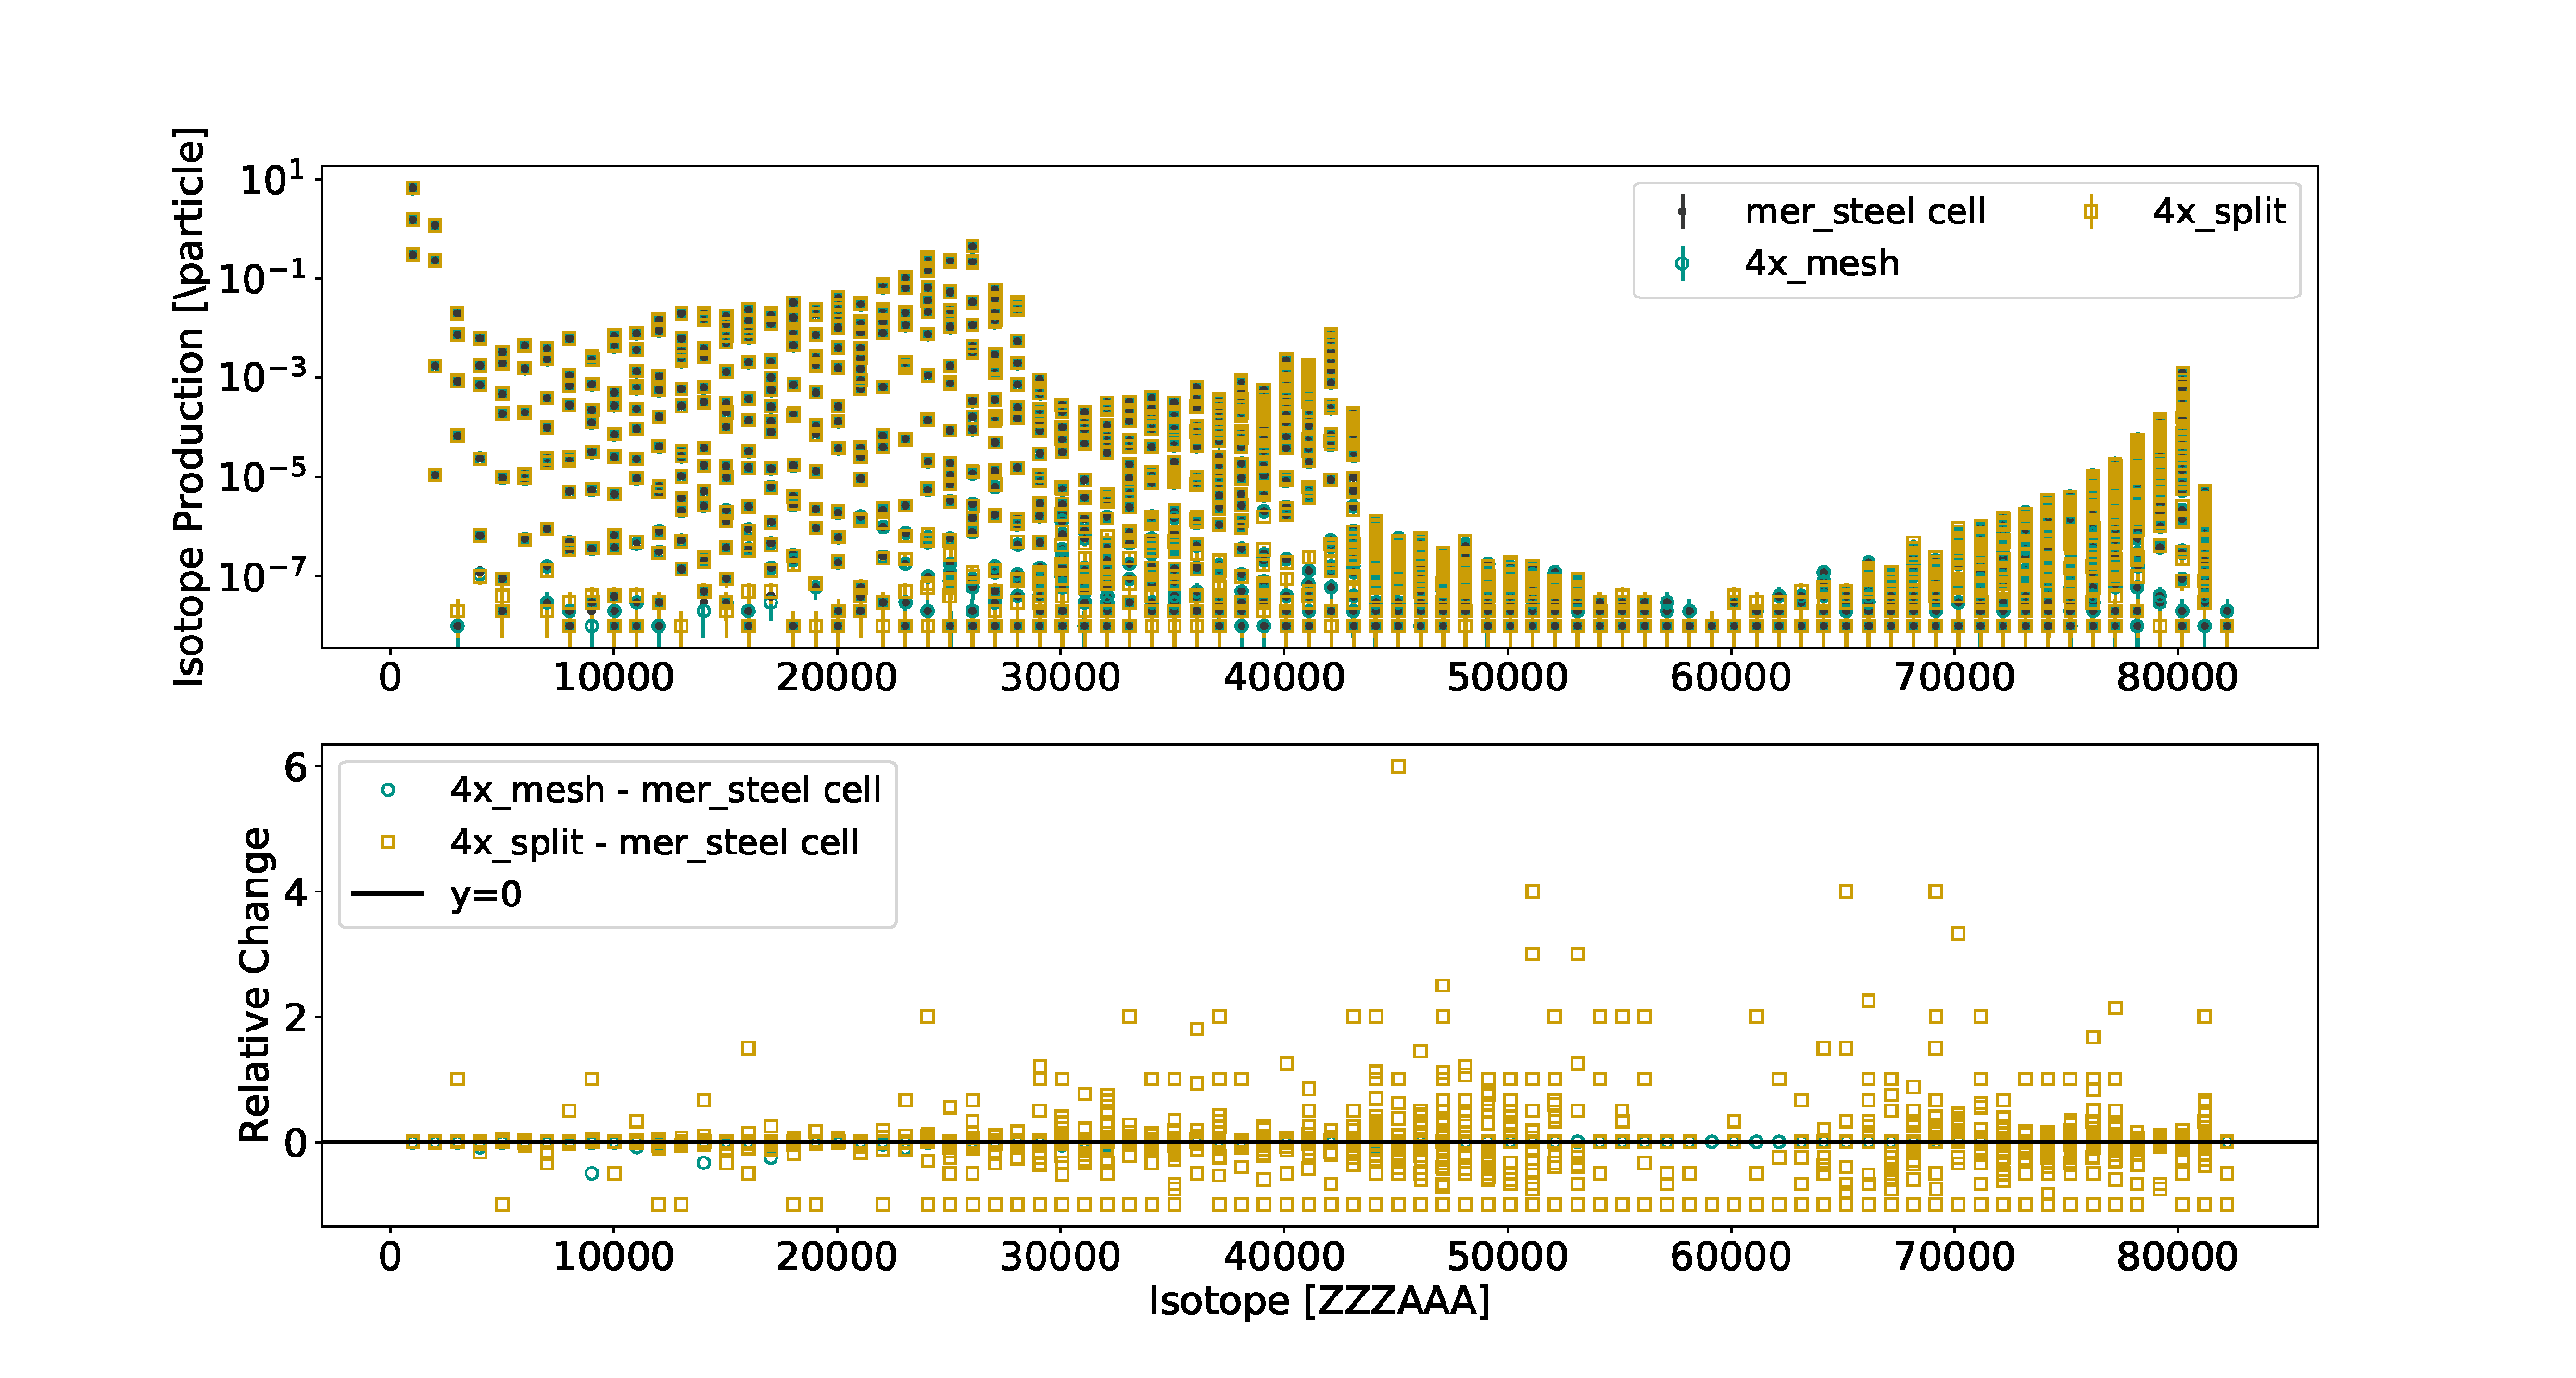
\includegraphics[scale=0.4,trim={2cm 1cm 3cm 2cm},clip]{../figs/toy_p2/prod_VPII_4x.pdf}
 \caption{Radionuclide production for mercury/steel cells, 4x4x4 mesh, and 4x4x4 divided geometry}
 \label{fig:2prod_cell_4x}
\end{figure}
%
\begin{figure}[H]
 \centering
 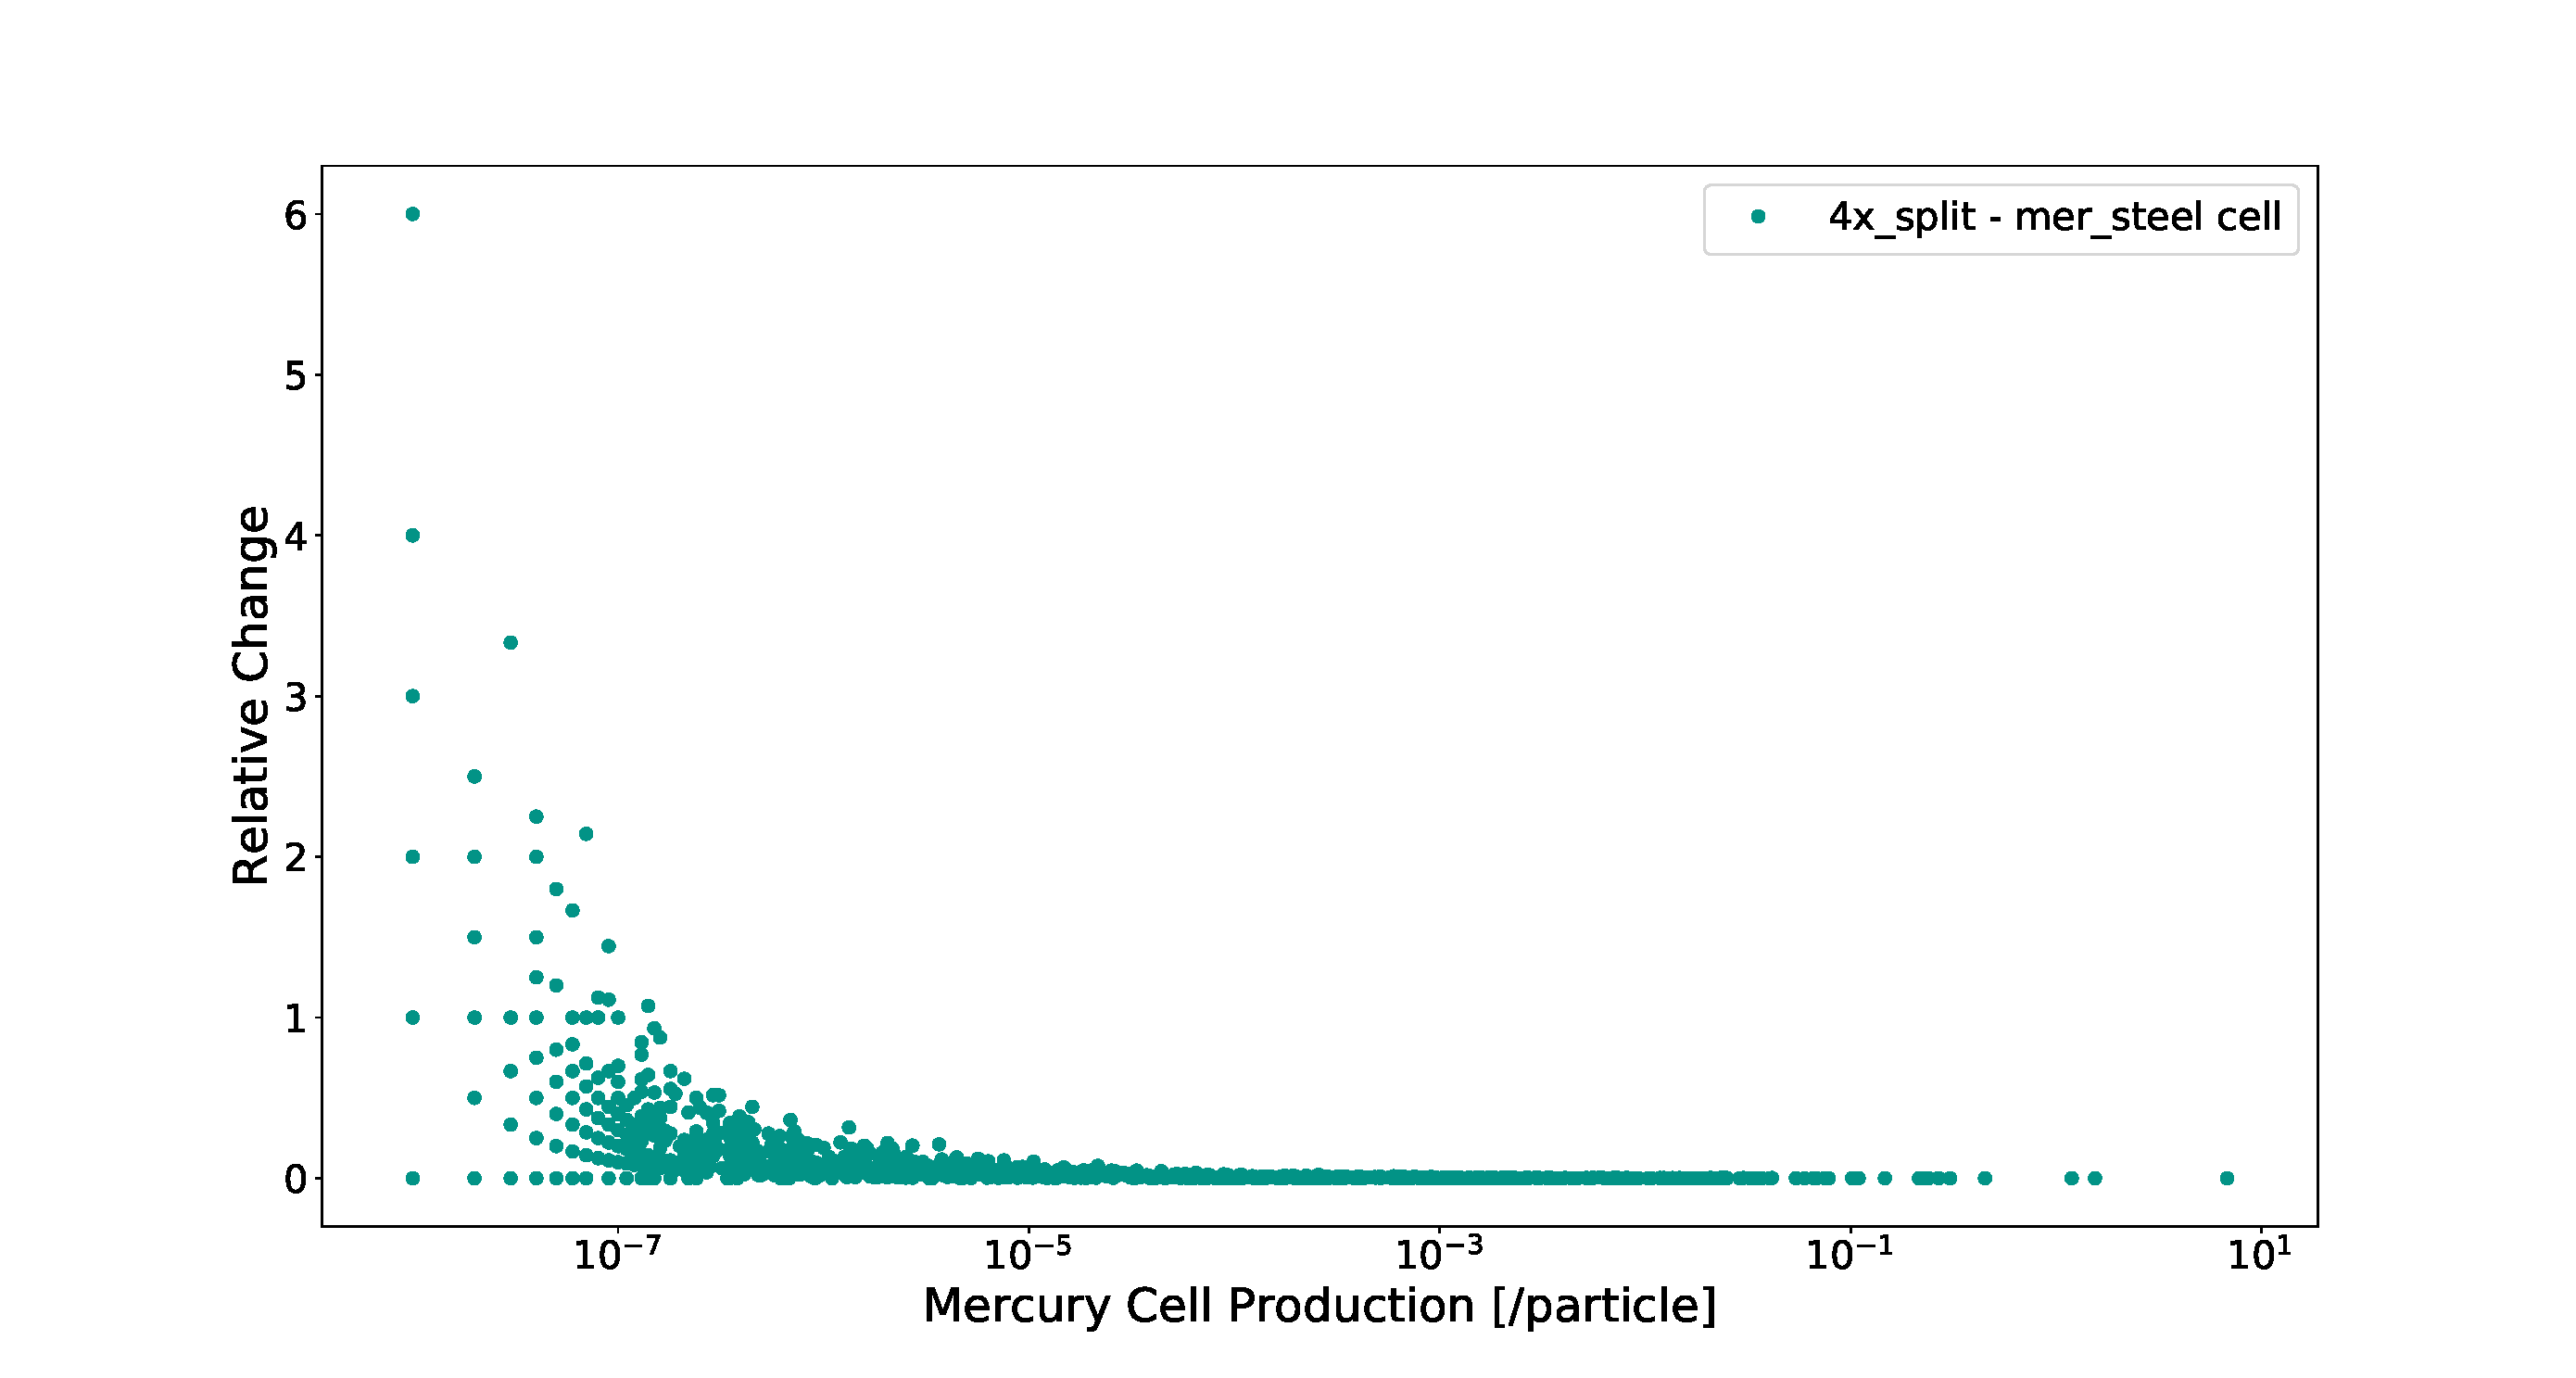
\includegraphics[scale=0.35,trim={3cm 0.5cm 4.5cm 3cm},clip]{../figs/toy_p2/prod_VPII_rc_4x_split.pdf}
 \caption{Relative change between cells and 4x4x4 geometry split vs. the isotope production of the mercury cell}
 \label{fig:2prod_cell_4x_rc}
\end{figure}
%
Figure \ref{fig:2spec_cell_1x_2x_4x} shows the photon density emission
collected in the mercury and steel volumes, and each of the meshes. The bottom
graph in the same figure shows the relative change when comparing the results
averaged over each of the meshes to the results of the mercury and steel cells.
\begin{figure}[H]
 \centering
 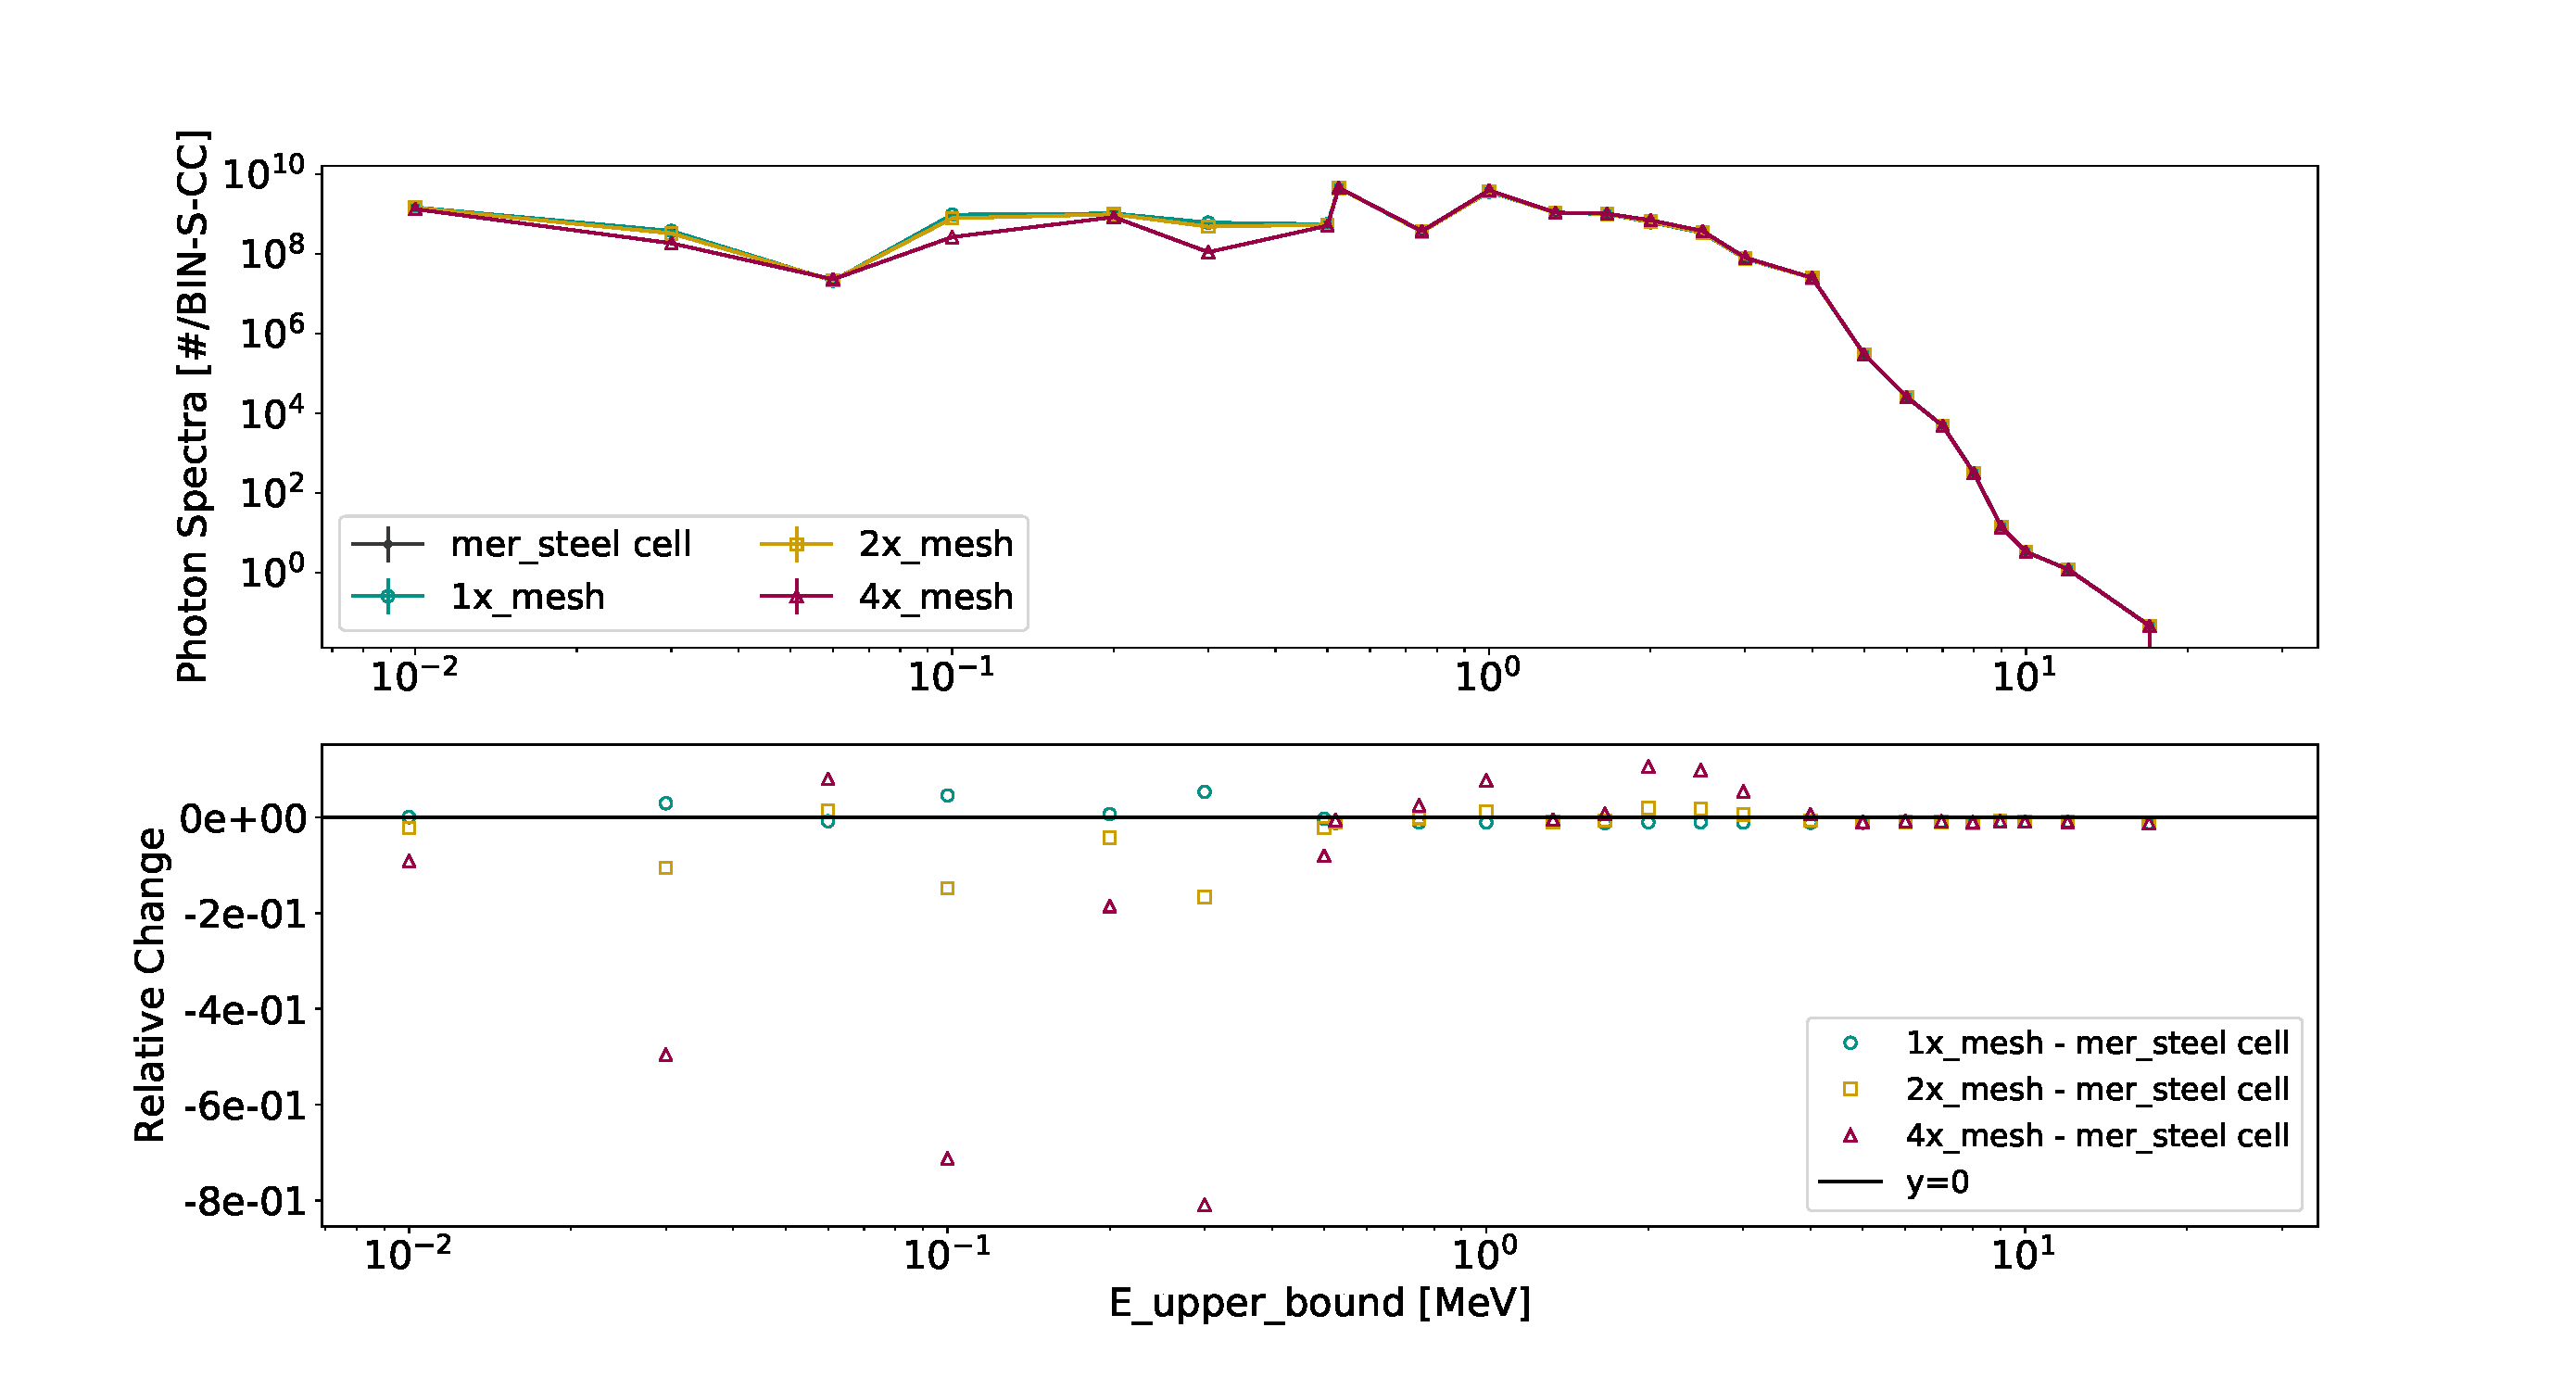
\includegraphics[scale=0.4,trim={2cm 0.5cm 3cm 2cm},clip]{../figs/toy_p2/spec_VPII_1x_2x_4x.pdf}
 \caption{Photon Spectrum in mercury/steel cell and different meshes}
 \label{fig:2spec_cell_1x_2x_4x}
\end{figure}
%
When comparing the photon emission density collected in the divided geometry
to the photon density collected in the mercury and steel, we can see that
there some large discrepancy between some of the results. This can be seen in
Figure \ref{fig:2spec_cell_2x}. Figure \ref{fig:2spec_cell_4x} shows similar
for the 4x4x4 divided geometry. In this case, the relative difference is a lot
smaller.
%
\begin{figure}[H]
 \centering
 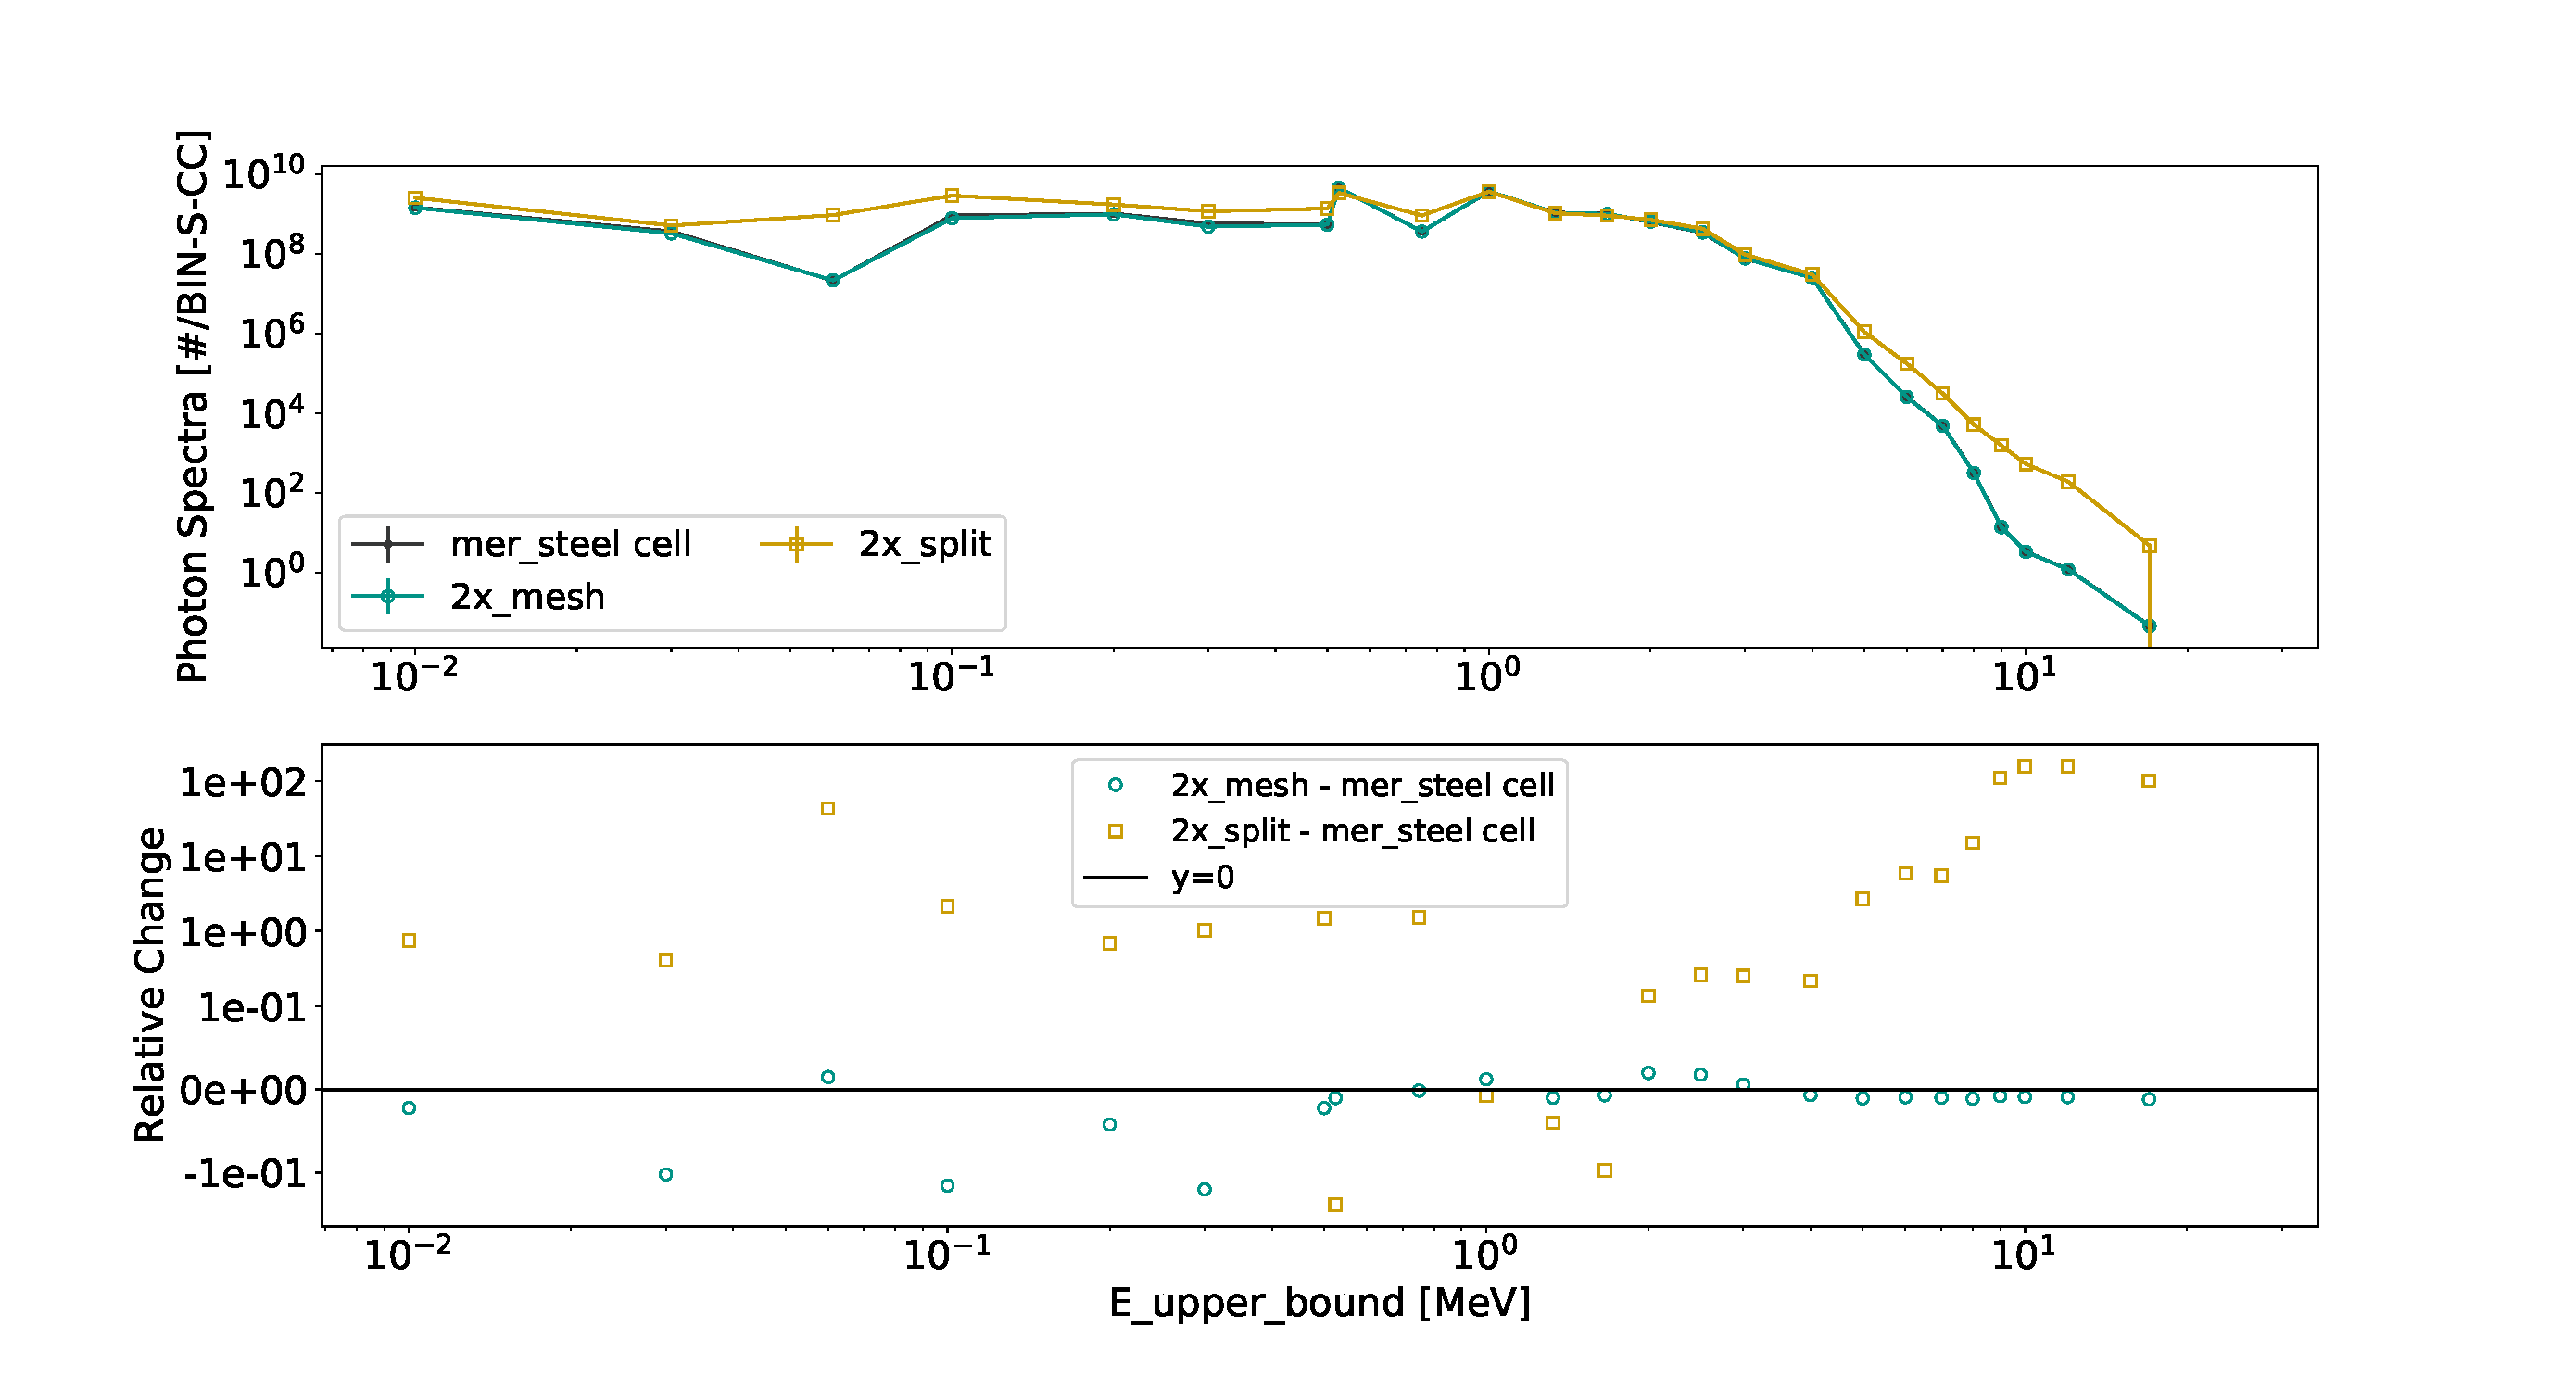
\includegraphics[scale=0.4,trim={2cm 0.5cm 3cm 2cm},clip]{../figs/toy_p2/spec_VPII_2x.pdf}
 \caption{Photon Spectrum in mercury cell, 2x2x2 mesh, and geometry split}
 \label{fig:2spec_cell_2x}
\end{figure}
%
\begin{figure}[H]
 \centering
 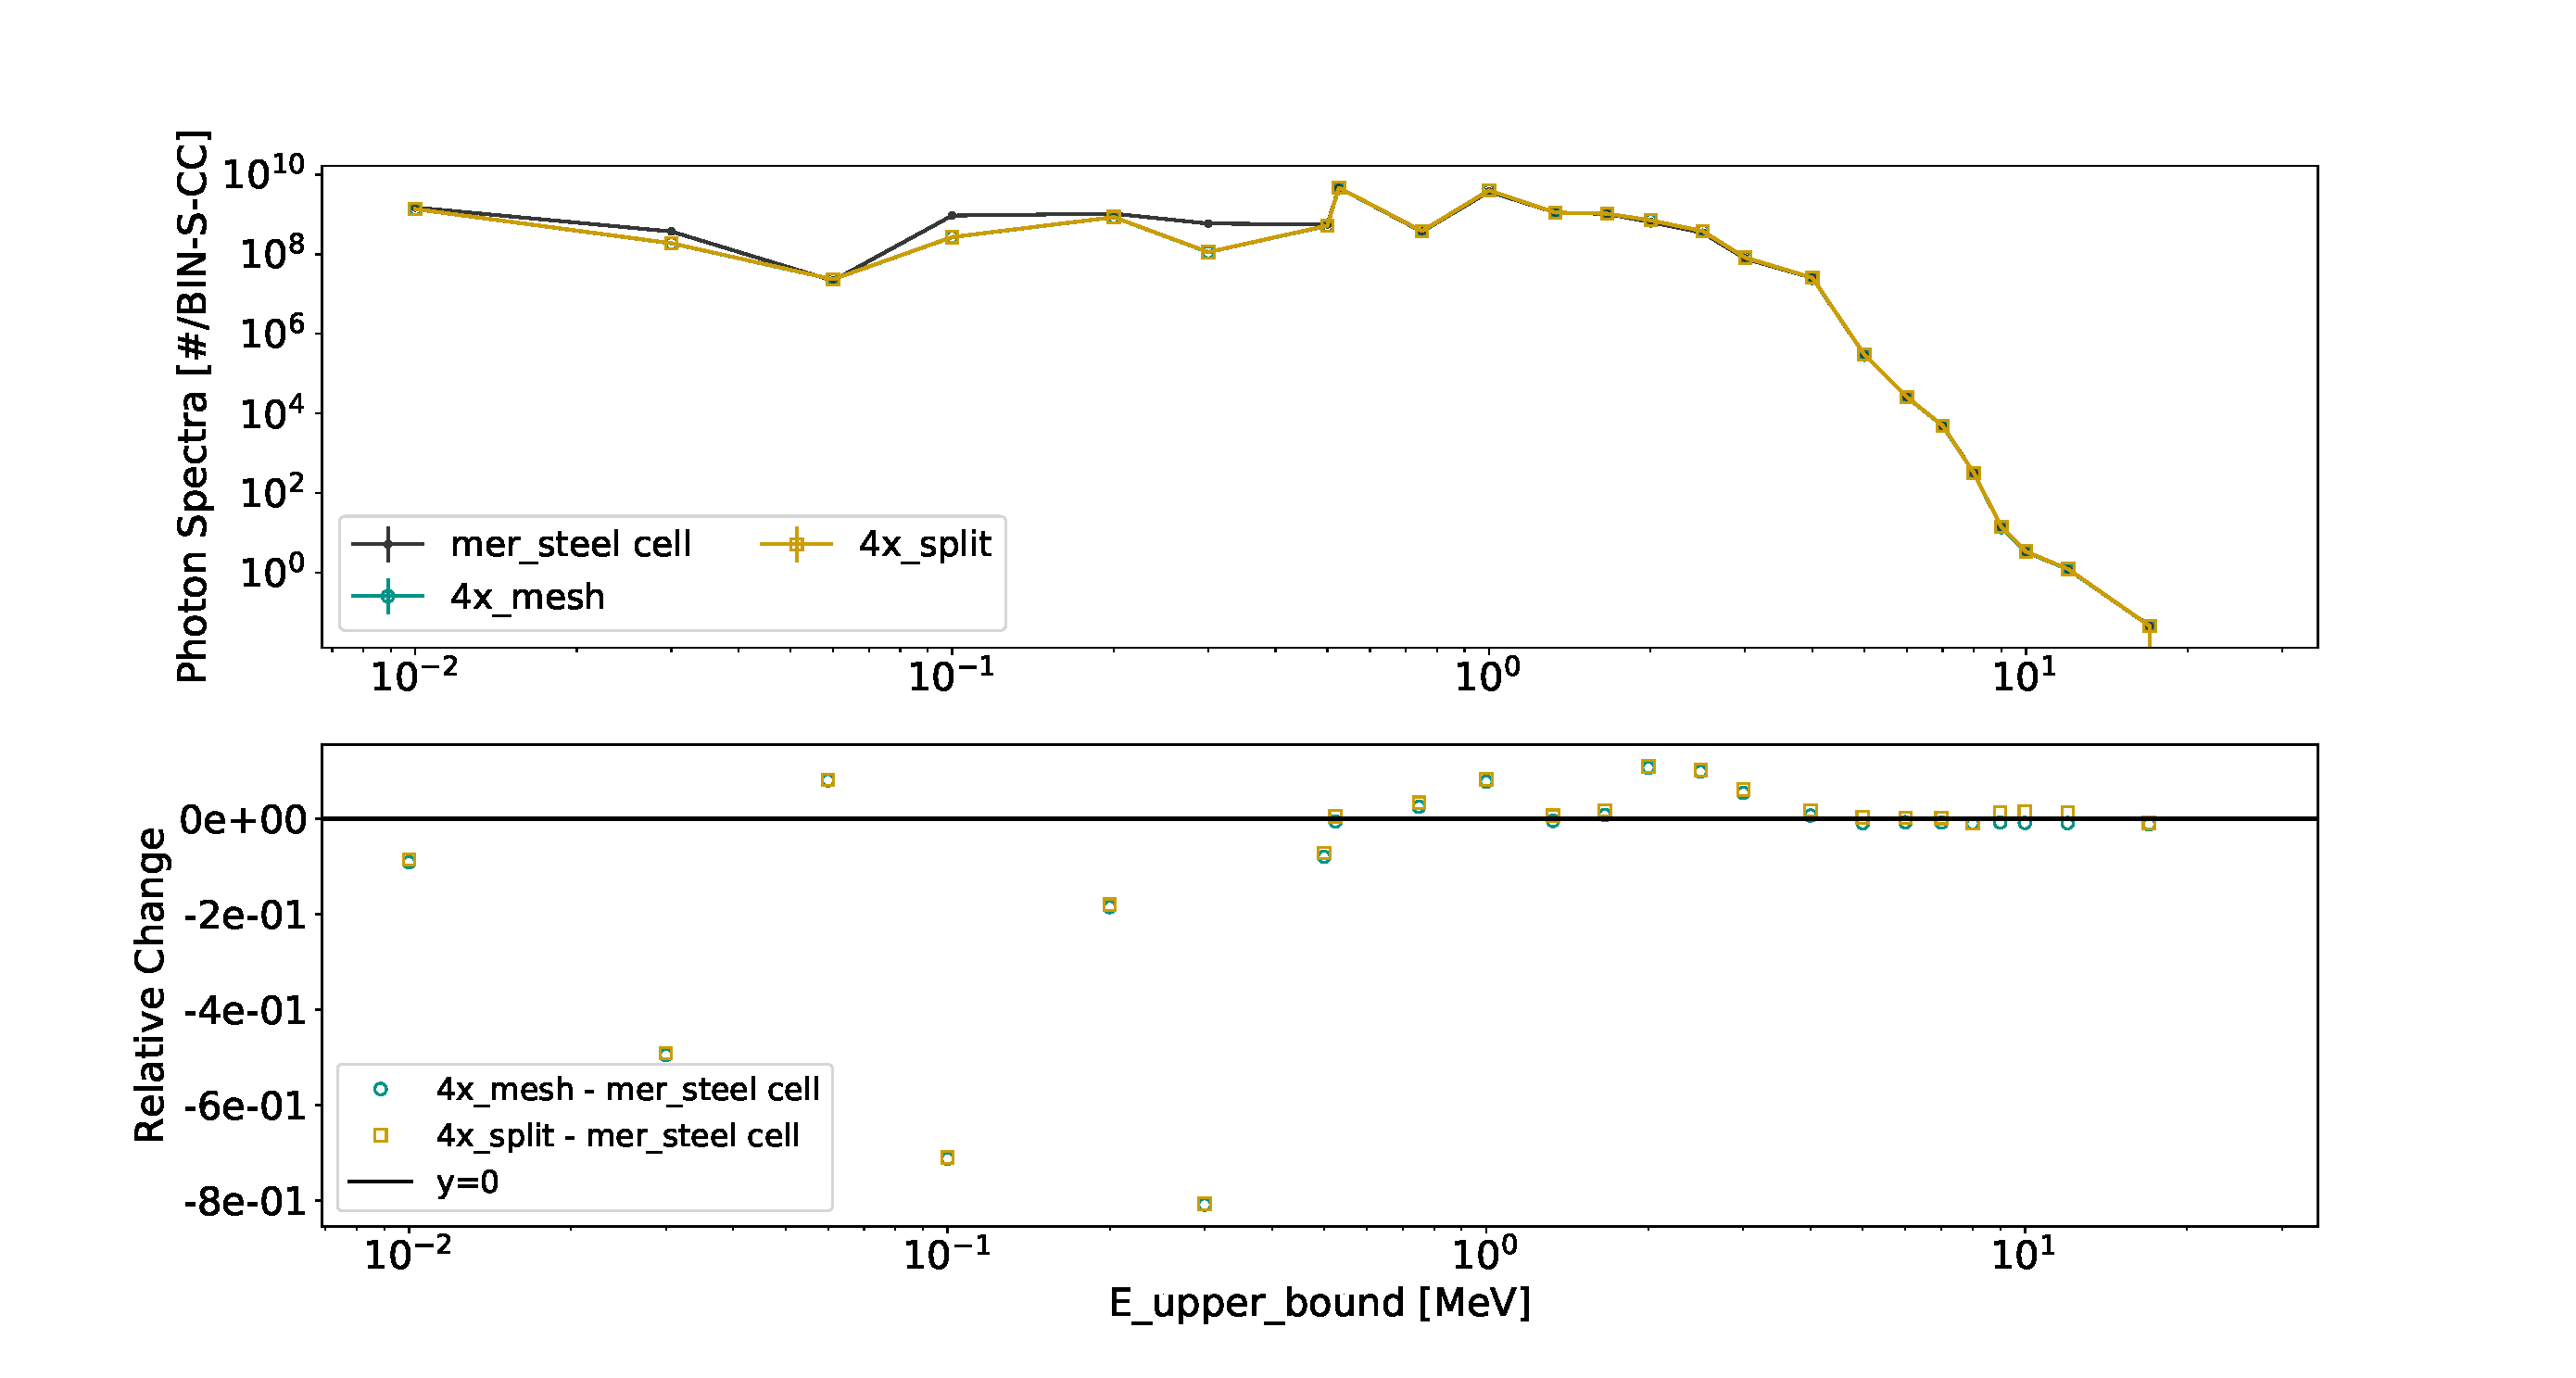
\includegraphics[scale=0.4,trim={2cm 0.5cm 3cm 2cm},clip]{../figs/toy_p2/spec_VPII_4x.pdf}
 \caption{Photon Spectrum in mercury/steel cell, 4x4x4 mesh, and geometry split}
 \label{fig:2spec_cell_4x}
\end{figure}
%
Figure \ref{fig:2spec_8v} shows photon emission density per voxel for a
2x2x2 mesh, and for combined mercury and steel cell. This graph shows higher
photon emission density for voxels 1, 3, 5, and 7 which are the voxels closer
to the proton source in the configuration of the first transport.
\begin{figure}[H]
        \begin{subfigure}[t]{1.0\textwidth}
                \hfill
                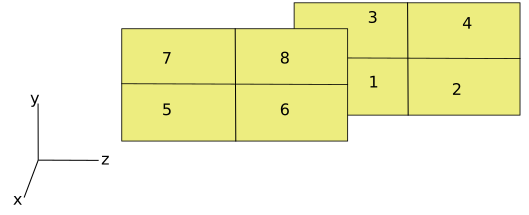
\includegraphics[scale=0.4, trim={0cm 0cm 0cm 0cm},clip]{../figs/voxels.png}
        \end{subfigure}\hfill
        \begin{subfigure}[t]{1.0\textwidth}
                \centering
                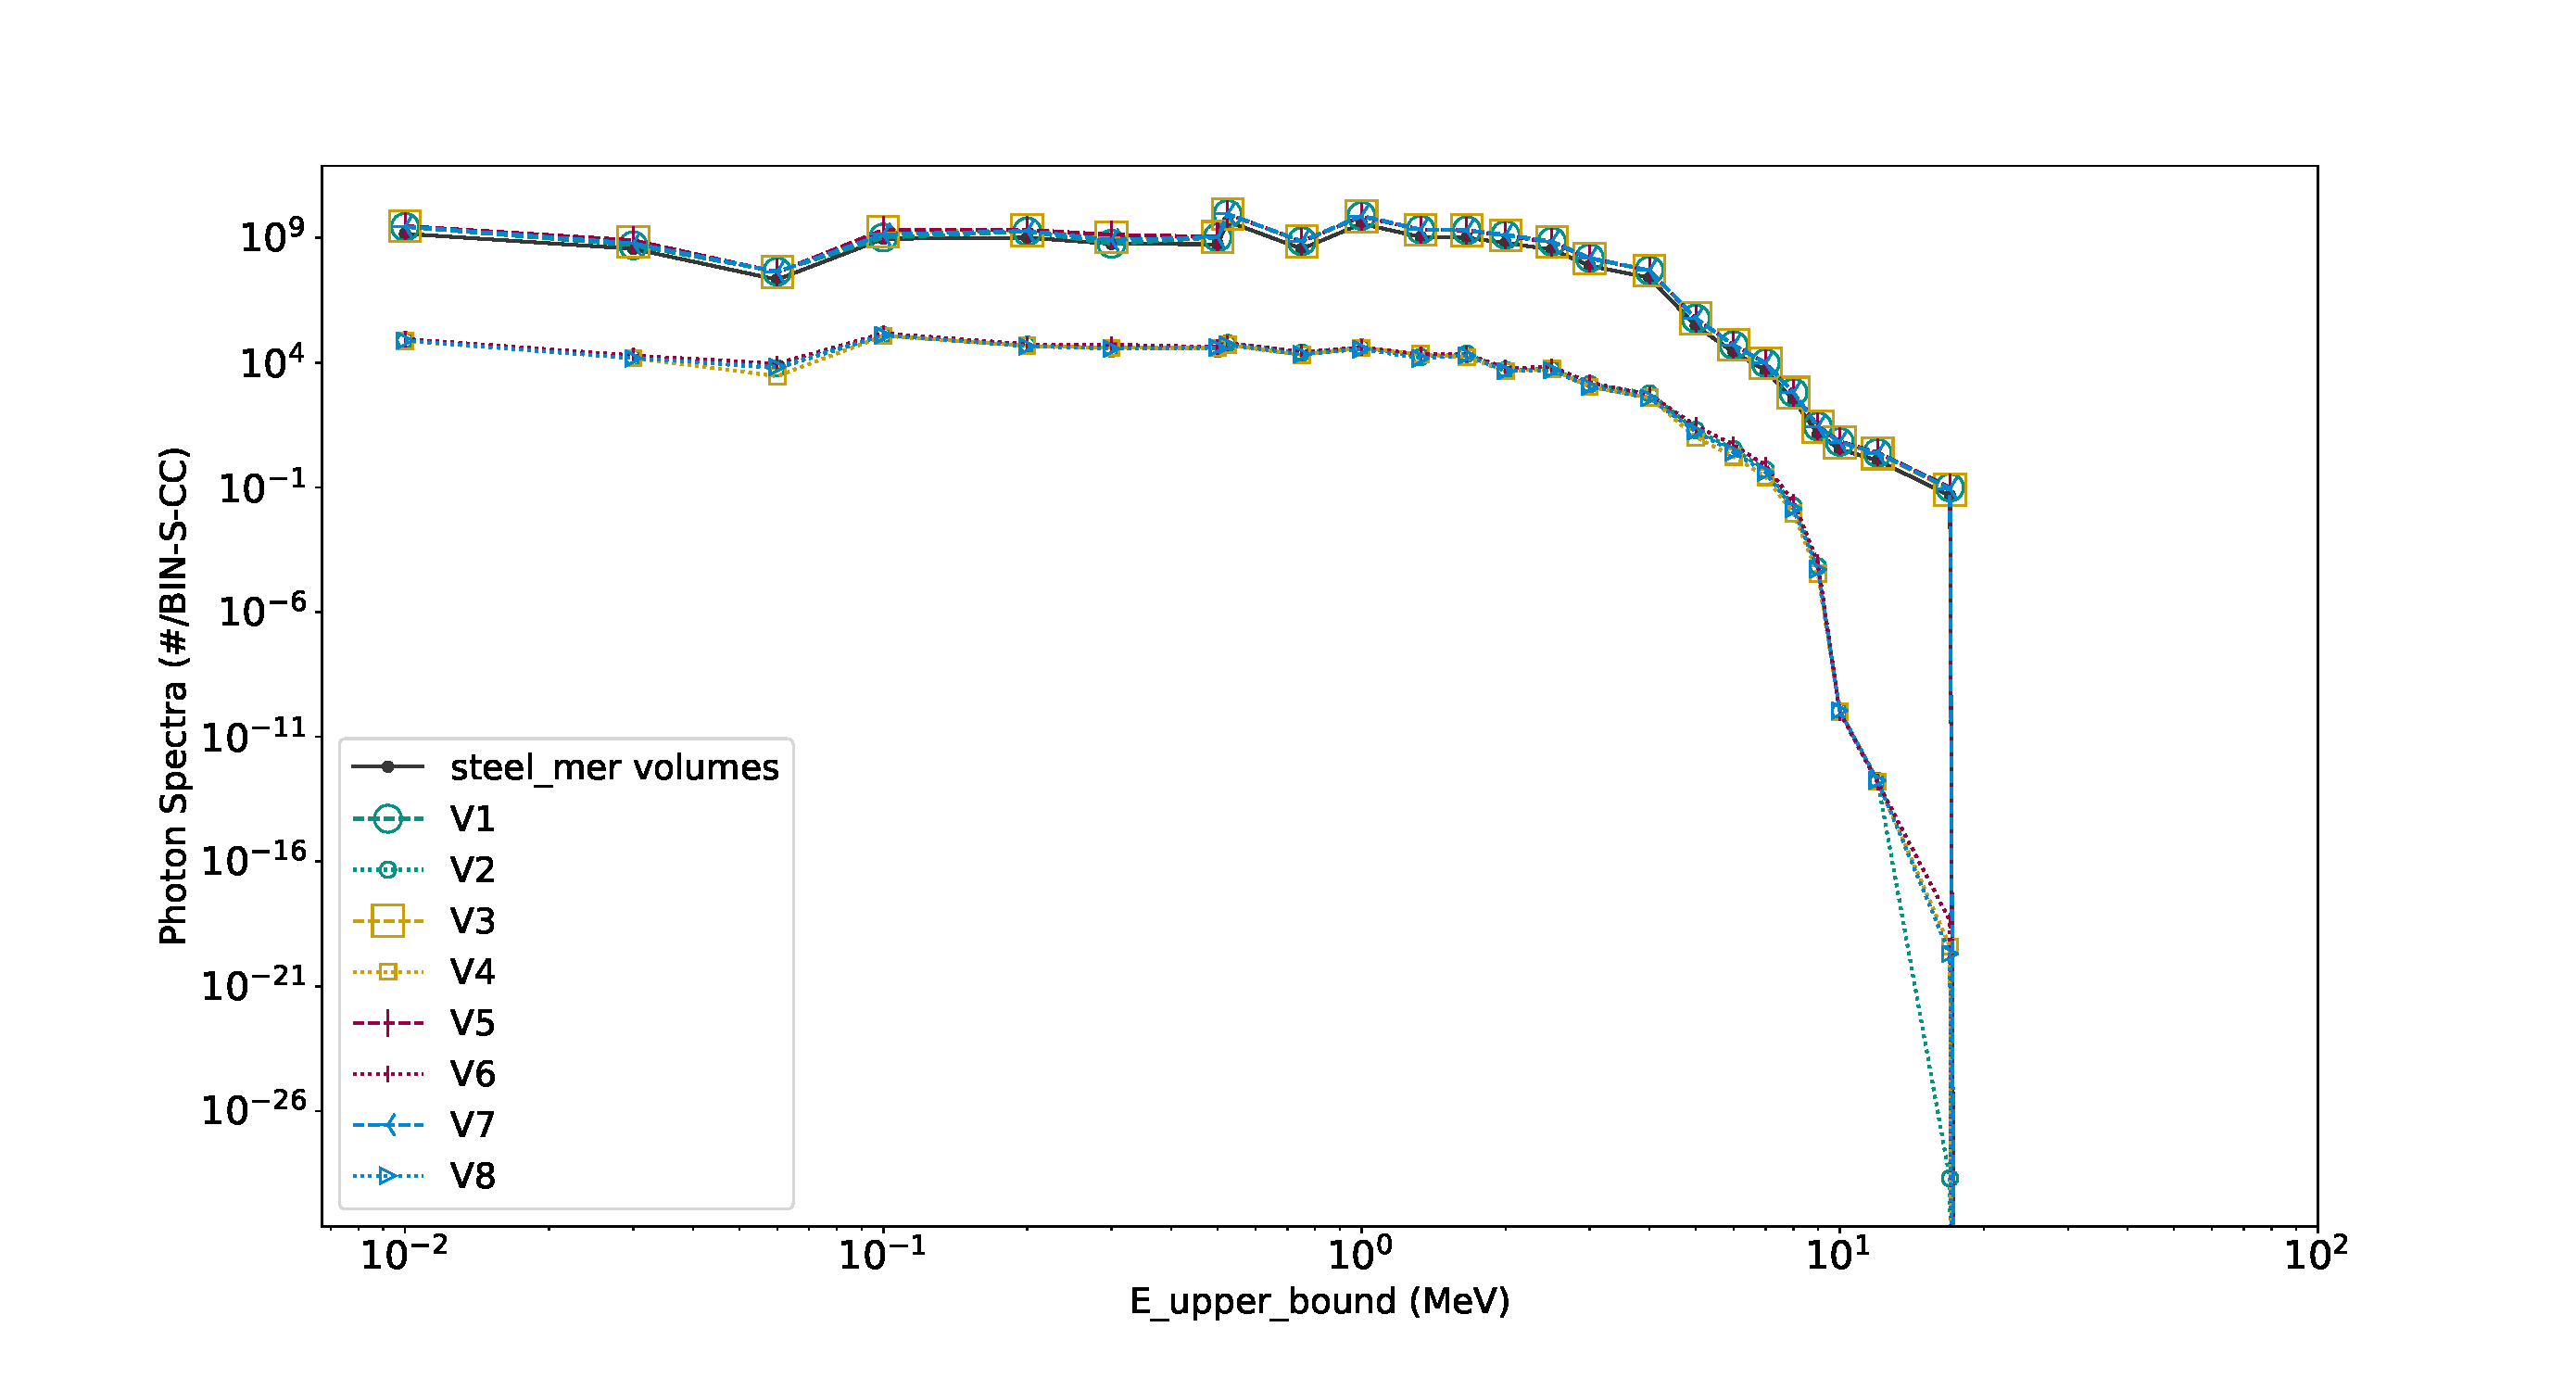
\includegraphics[scale=0.4, trim={2.5cm 1cm 3cm 3cm},clip]{../figs/toy_p2/spec_VPII_8.pdf}
        \end{subfigure}
        \caption{Photon emission density per voxel in a 2x2x2 mesh and the mercury/steel volumes}
        \label{fig:2spec_8v}
\end{figure}
%
The photon emission density collected using the cells of the original problem,
the cells of the divided geometry, and the superimposed mesh was used as the
photon source in the photon transport.
The biological dose rate was collected in a superimposed mesh spanning the
entire geometry.
%
\begin{figure}[H]
	\begin{subfigure}[t]{0.5\textwidth}
		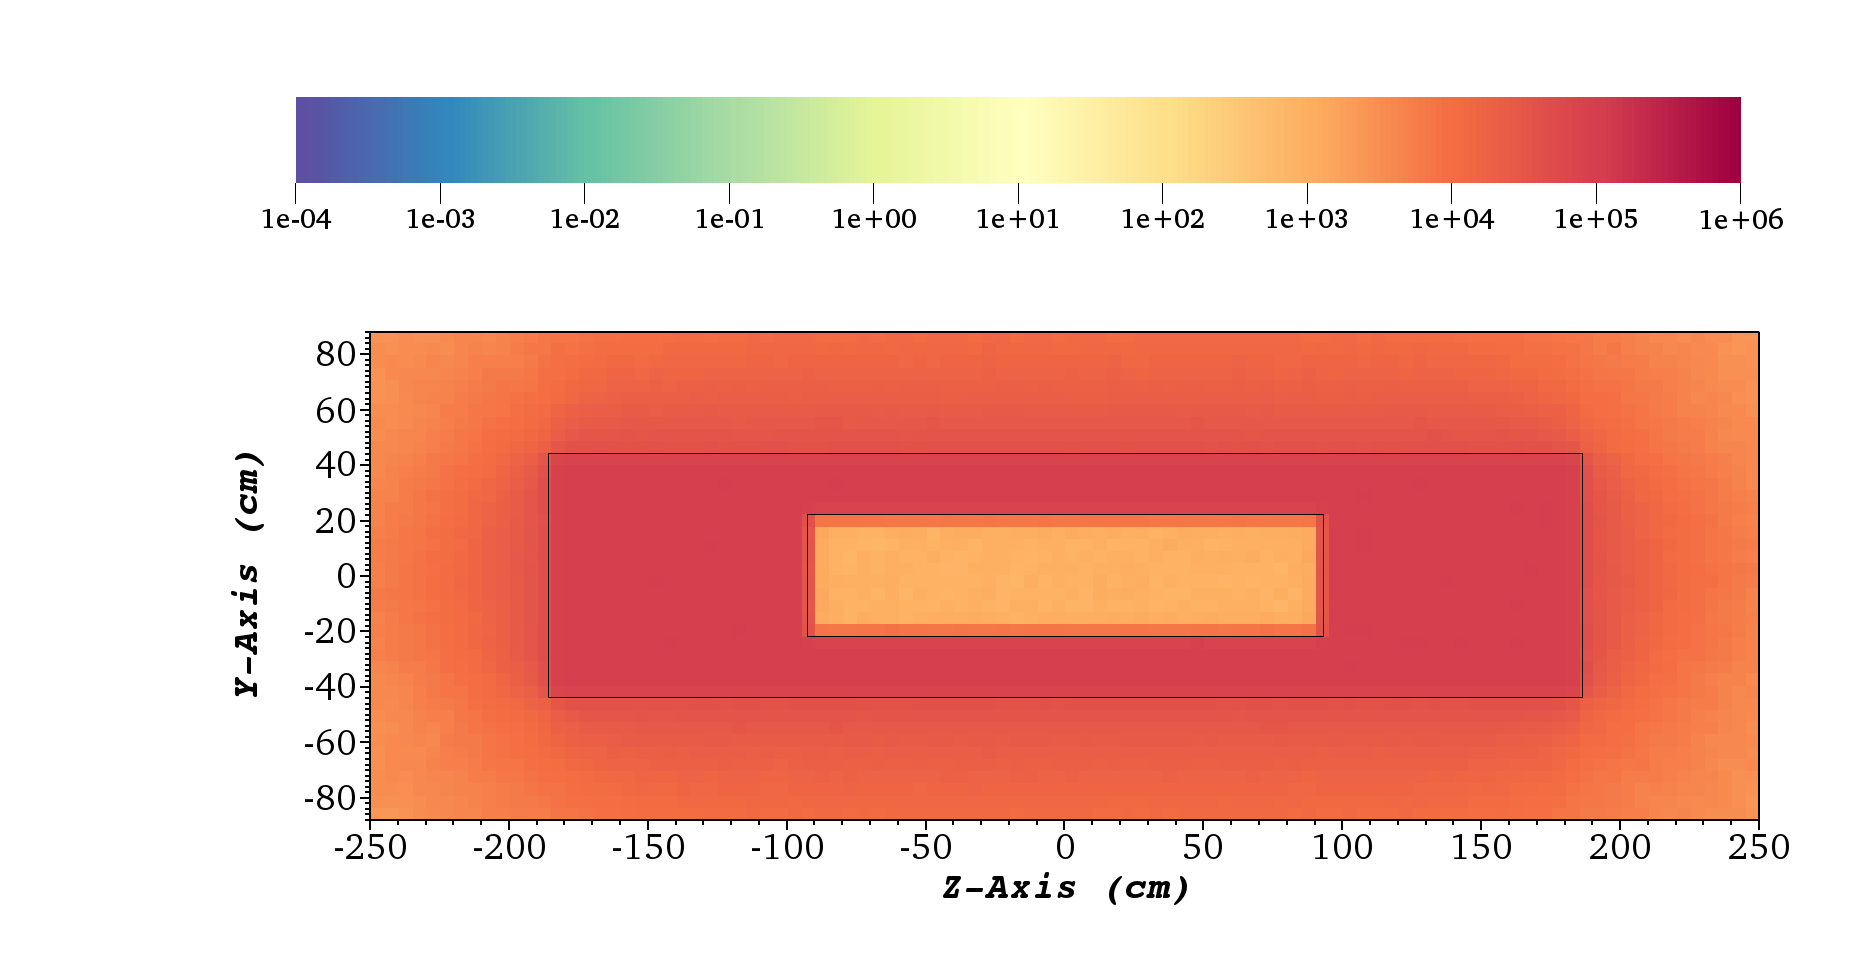
\includegraphics[width=\linewidth, trim={8cm 2cm 2cm 10cm},clip]{../figs/toy_p2/dose_VPII_original.png}
		\caption{full geometry}
		\label{fig:2dose_orig}
	\end{subfigure}\hfill
	\begin{subfigure}[t]{0.5\textwidth}
		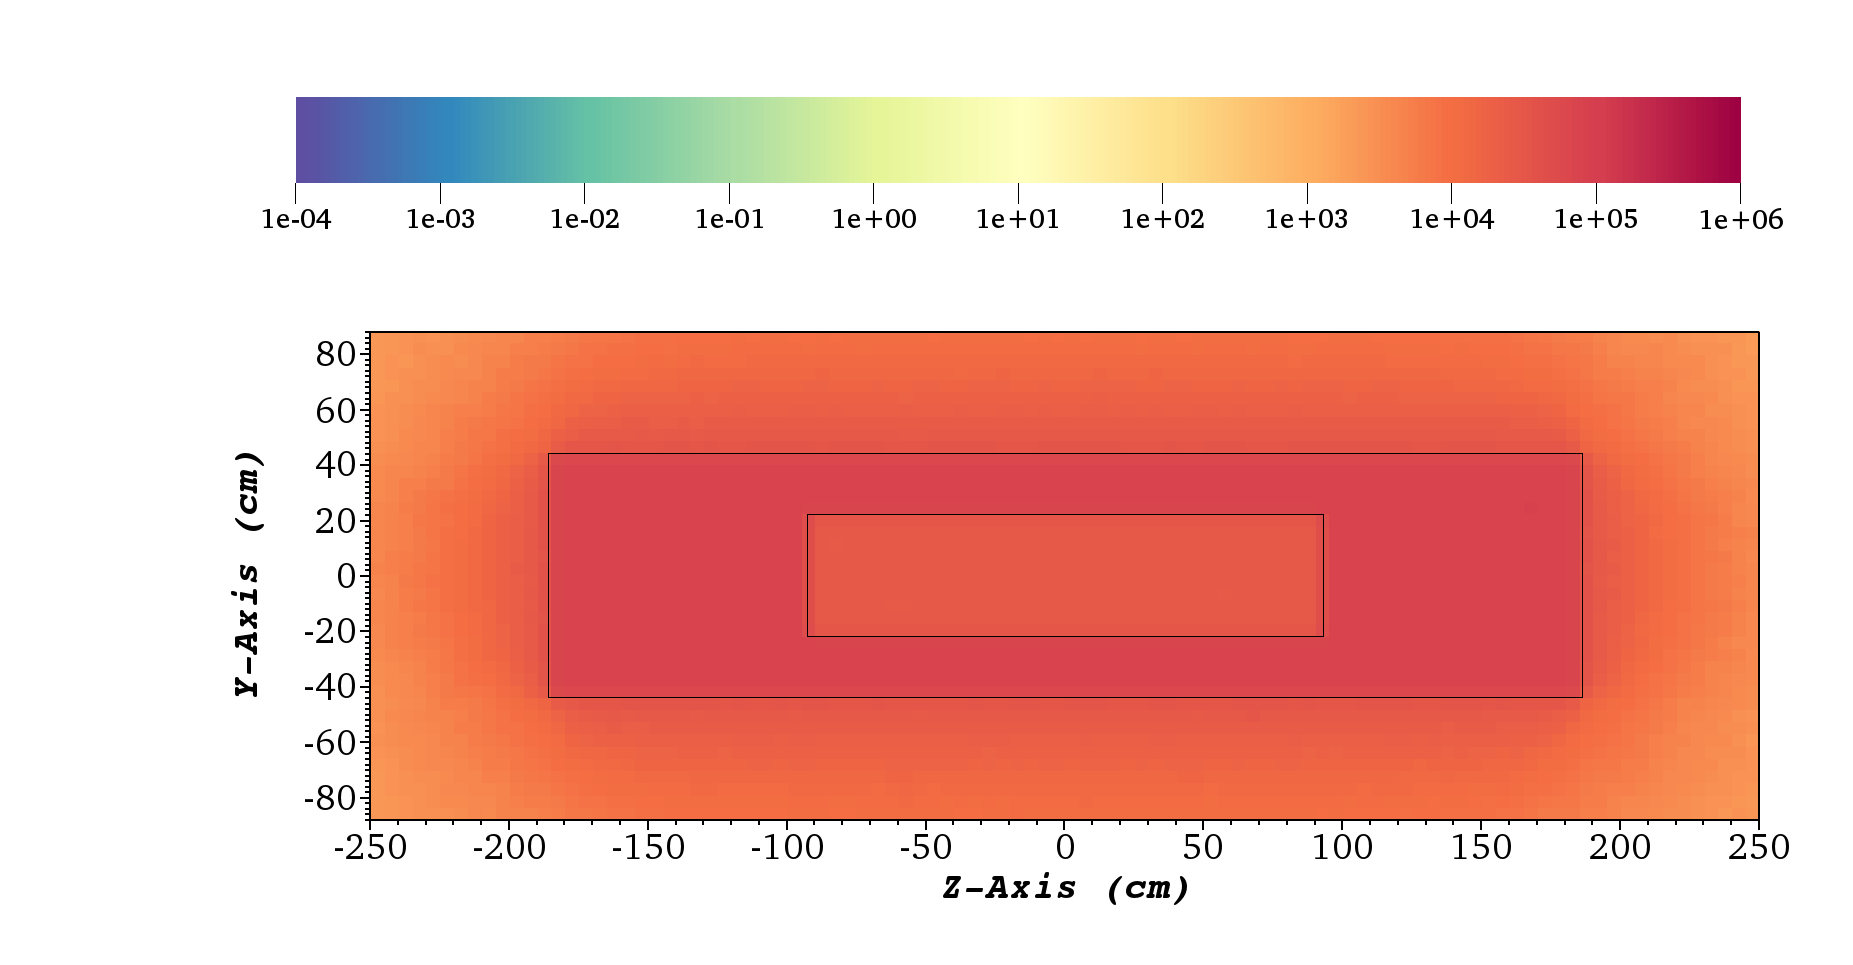
\includegraphics[width=\linewidth, trim={8cm 2cm 2cm 10cm},clip]{../figs/toy_p2/dose_VPII_1x_mesh.png}
		\caption{1x1x1 mesh}
		\label{fig:2dose_1x_mesh}
	\end{subfigure}

	\begin{subfigure}[t]{0.5\textwidth}
		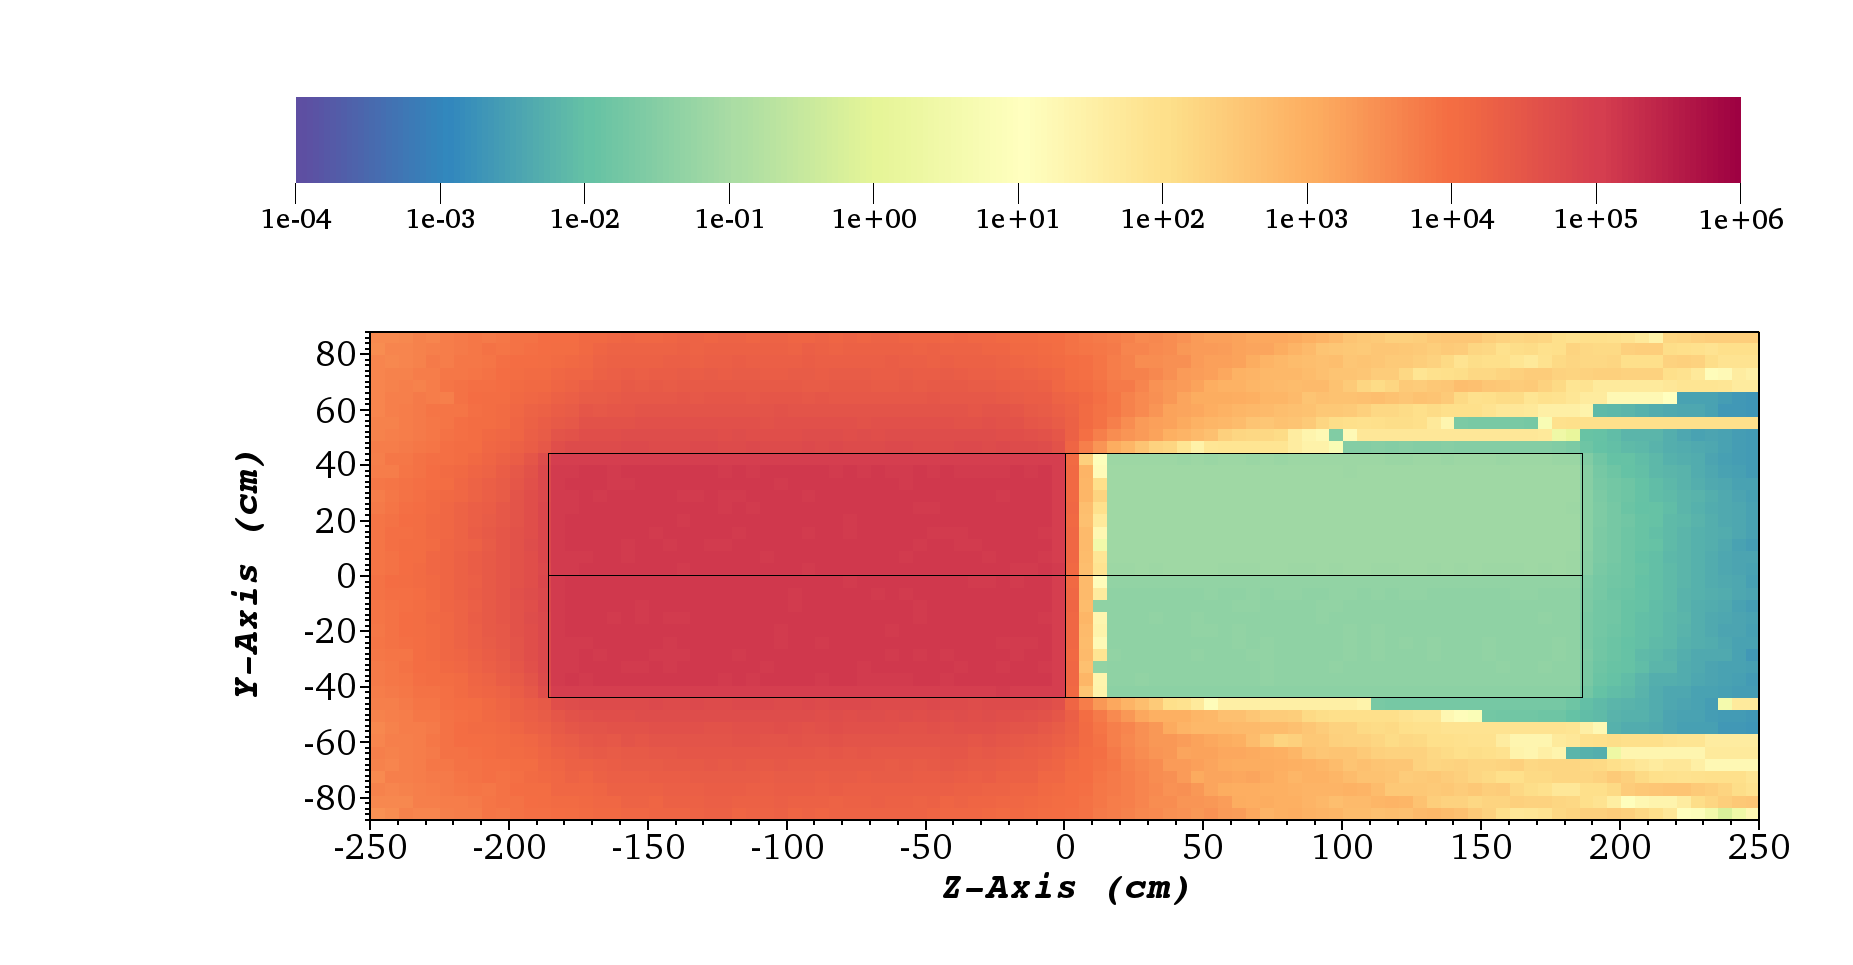
\includegraphics[width=\linewidth, trim={8cm 2cm 2cm 10cm},clip]{../figs/toy_p2/dose_VPII_2x_split.png}
		\caption{2x2x2 divided}
		\label{fig:2dose_2x_split}
	\end{subfigure}\hfill
	\begin{subfigure}[t]{0.5\textwidth}
		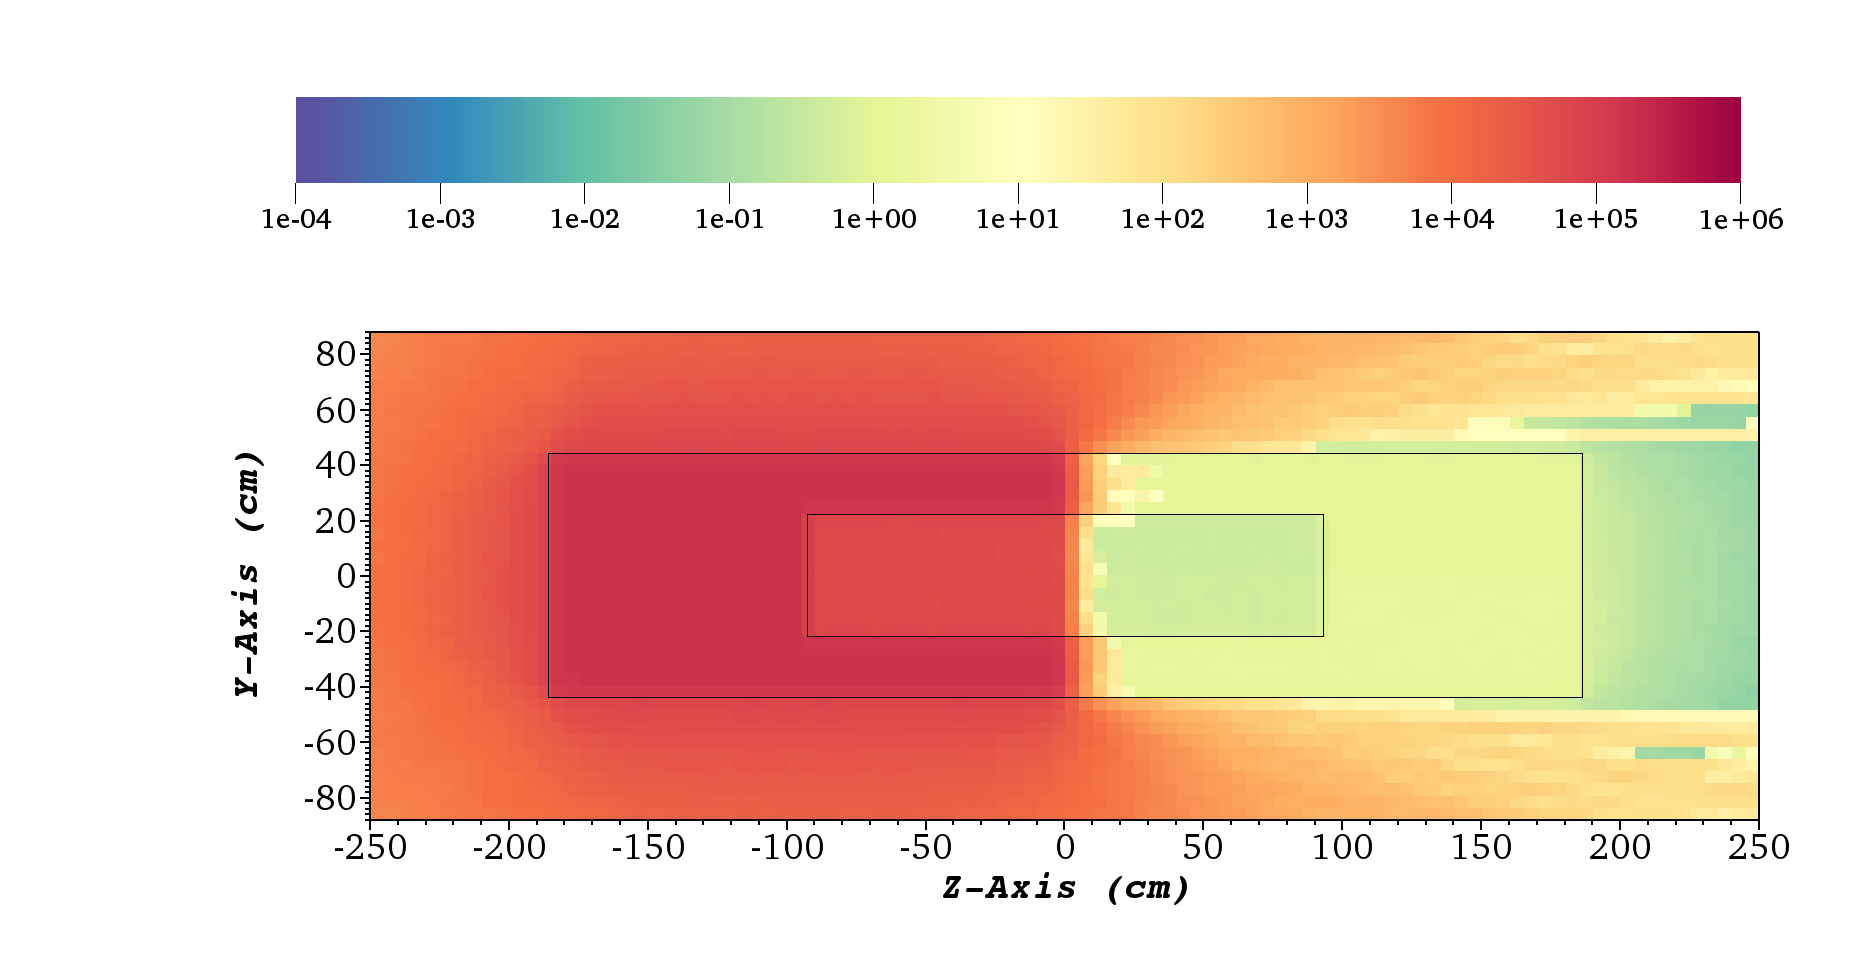
\includegraphics[width=\linewidth, trim={8cm 2cm 2cm 10cm},clip]{../figs/toy_p2/dose_VPII_2x_mesh.png}
		\caption{2x2x2 mesh}
		\label{fig:2dose_2x_mesh}
	\end{subfigure}

	\begin{subfigure}[t]{0.5\textwidth}
		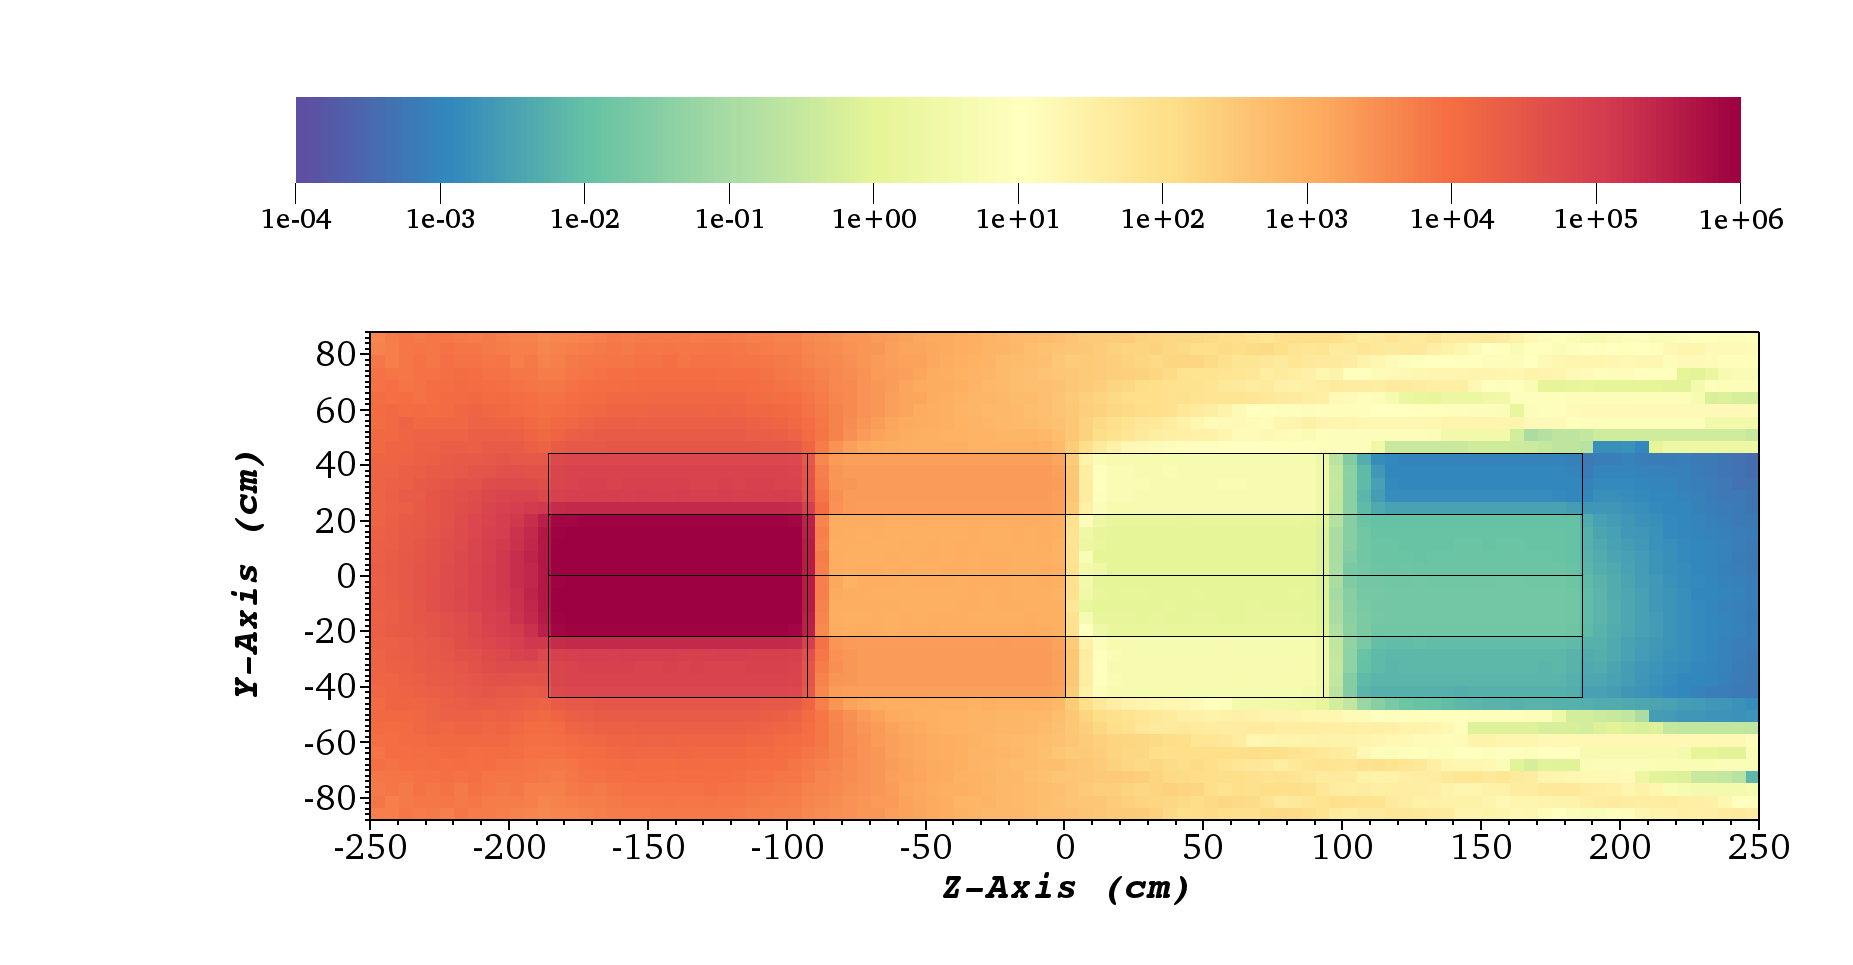
\includegraphics[width=\linewidth, trim={8cm 2cm 2cm 10cm},clip]{../figs/toy_p2/dose_VPII_4x_split.png}
		\caption{4x4x4 divided}
		\label{fig:2dose_4x_split}
	\end{subfigure}\hfill
	\begin{subfigure}[t]{0.5\textwidth}
		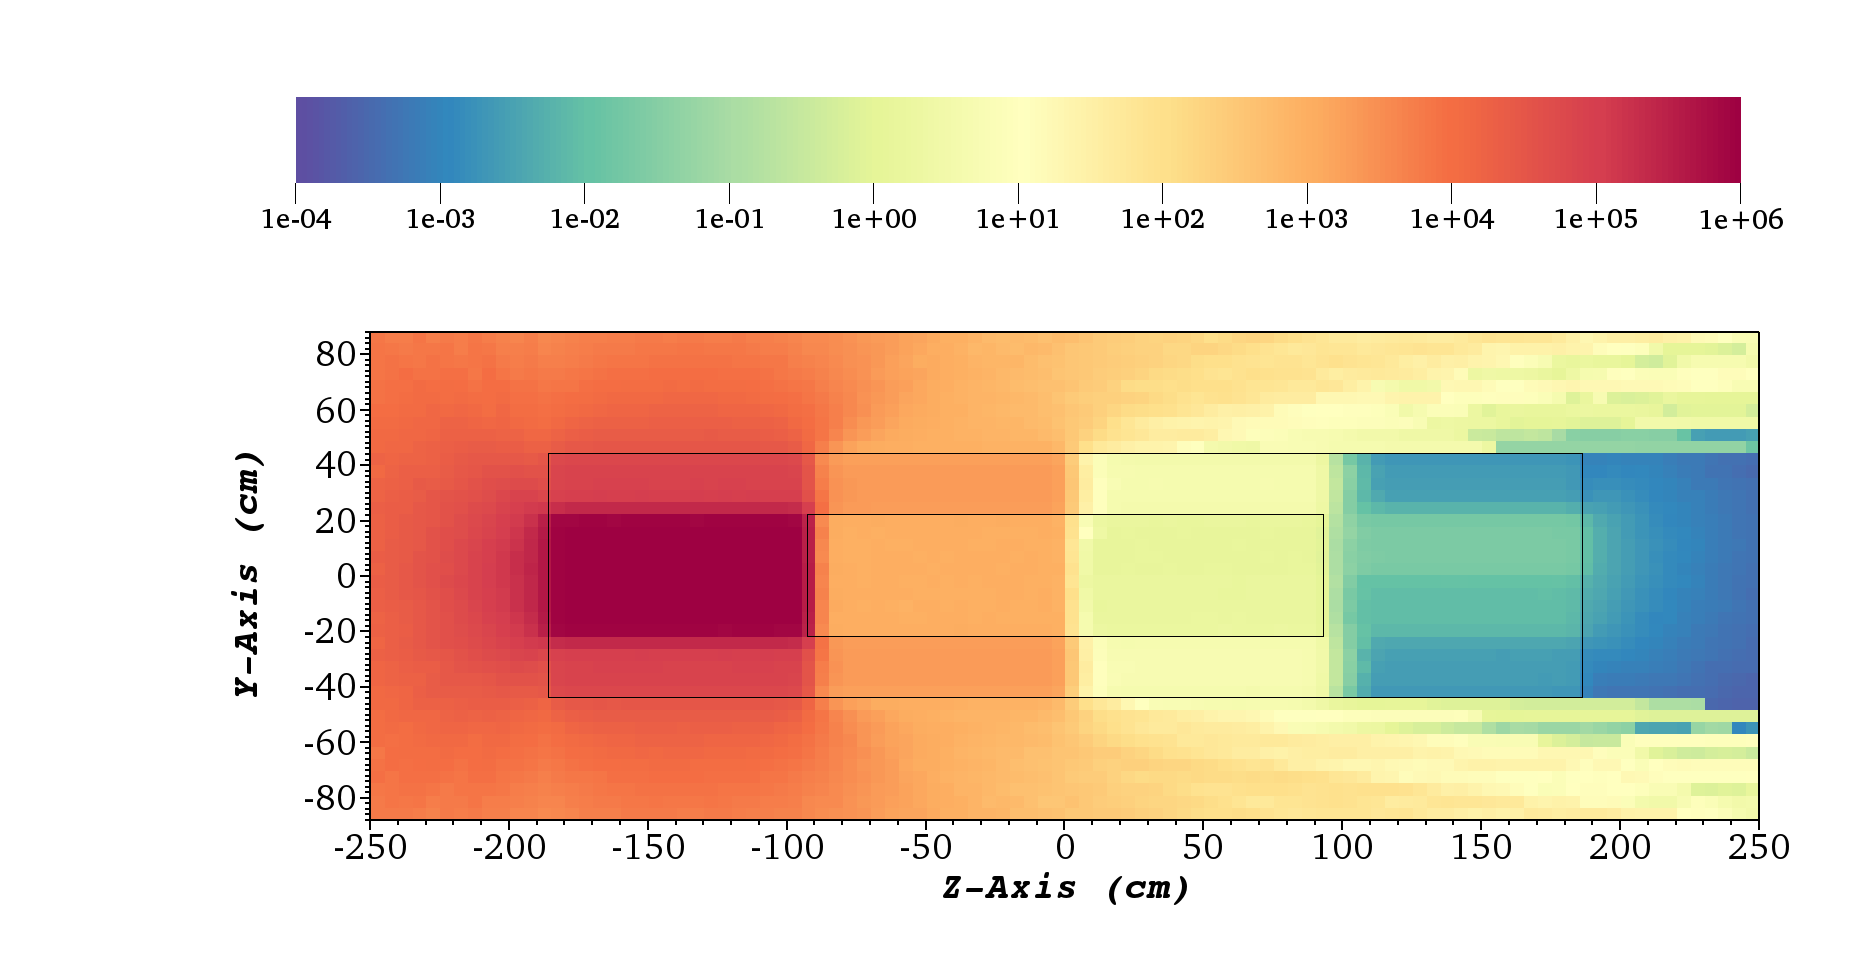
\includegraphics[width=\linewidth, trim={8cm 2cm 2cm 10cm},clip]{../figs/toy_p2/dose_VPII_4x_mesh.png}
		\caption{4x4x4 mesh}
		\label{fig:2dose_4x_mesh}
	\end{subfigure}

	\begin{subfigure}[t]{1.0\textwidth}
		\centering
		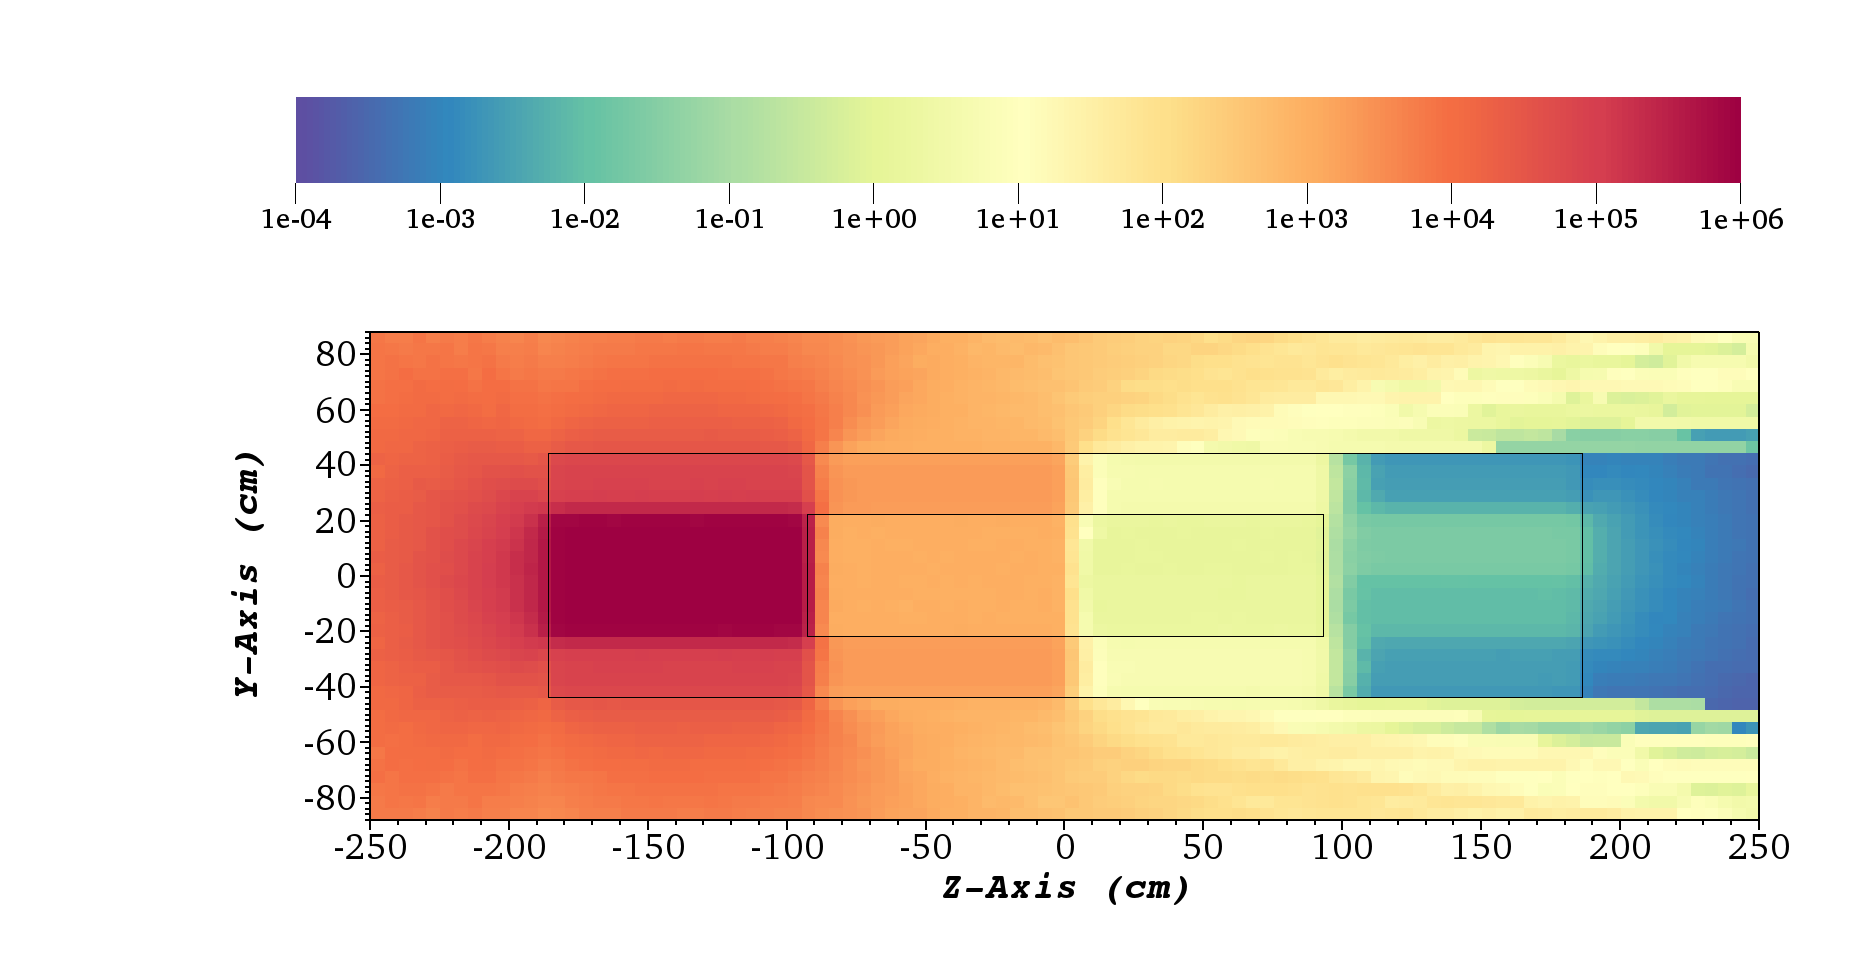
\includegraphics[width=\linewidth, trim={8cm 26cm 2cm 2cm},clip]{../figs/toy_p2/dose_VPII_4x_mesh.png}
		\label{fig:2legend}
	\end{subfigure}
	\caption{Biological dose rate on the mercury and steel cell with mesh and divided geometry}
	\label{fig:2dose}
\end{figure}
A z score was done to compare between the results from the mesh workflow and the results
obtained with the cell based workflow. The results can be seen in Figure \ref{fig:2zscores}.
Figure \ref{fig:2zscores} shows significant differences between results obtained
for the combined mercury and steel volumes and the results for the 1x1x1 mesh. This is
likely happening due to the way that the activation calculation is handled in each
workflow. In the case of the cell based workflow, the activation is done separately
for the mercury volume and for the steel volume. For the mesh based workflow, the
activation is performed for the per voxel. In the case of the 1x1x1 mesh, there
is only one mesh voxel, and it contains both materials in them. This means that
materials are mixed and a singular photon emission density is calculated
%
\begin{figure}[H]
	\begin{subfigure}[h]{1.0\textwidth}
		\centering
		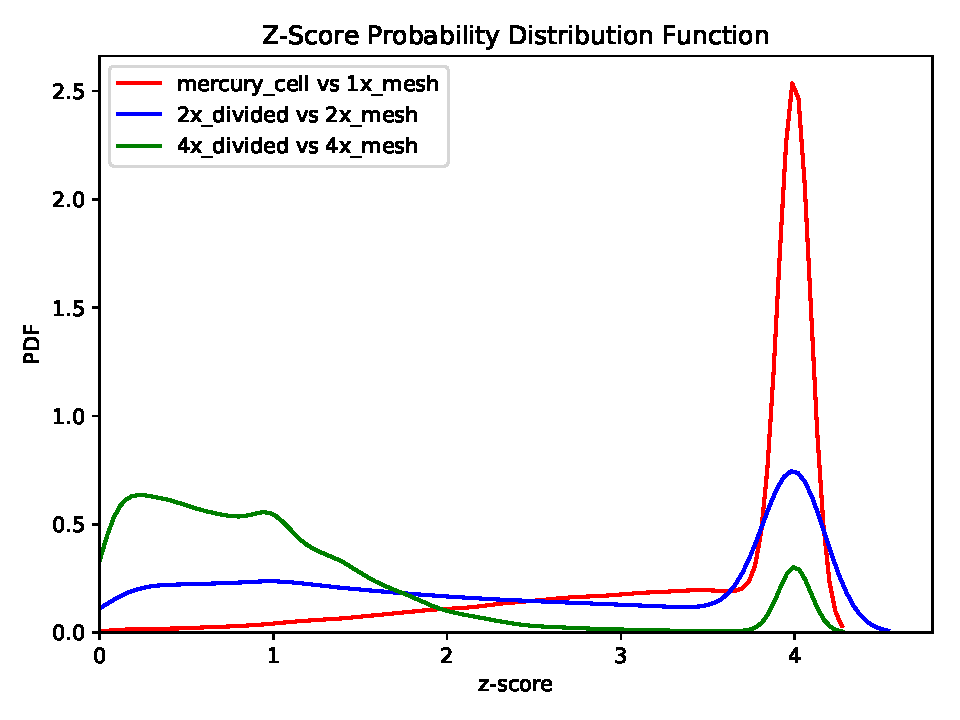
\includegraphics[scale=0.85, trim={0cm 0cm 0cm 0.9cm},clip]{../figs/toy_p2/PDF_zscore_VPII_all.pdf}
		\caption{Probability Density Function}
		\label{fig:2VPII_pdf}
	\end{subfigure}
	\begin{subfigure}[h]{1.0\textwidth}
		\centering
		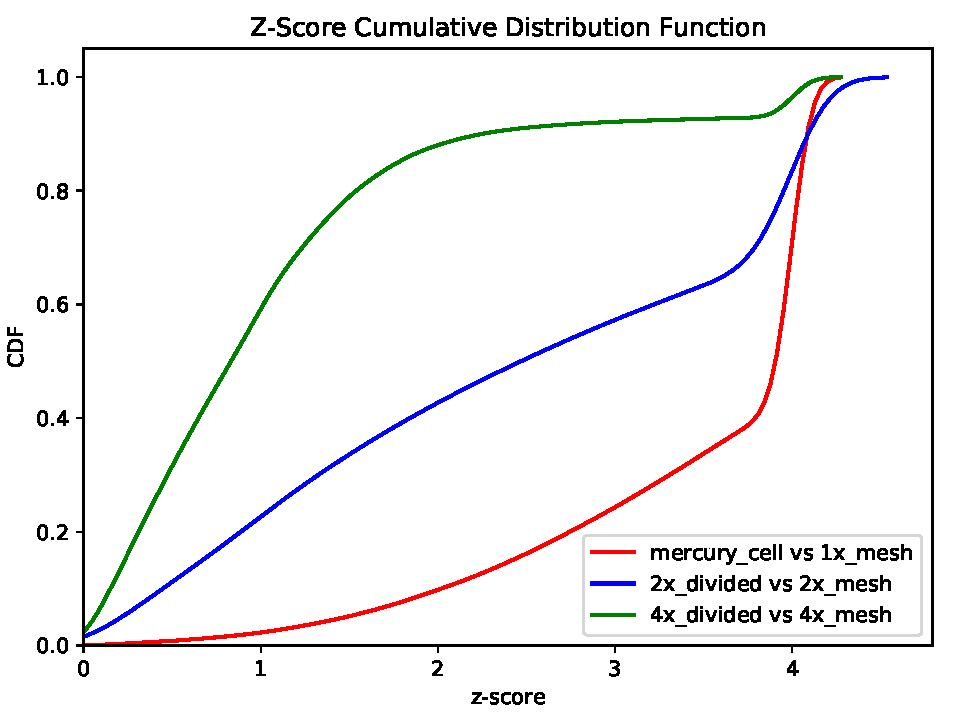
\includegraphics[scale=0.85, trim={0cm 0cm 0cm 0.8cm},clip]{../figs/toy_p2/CDF_zscore_VPII_all.pdf}
		\caption{Probability Density Function}
		\label{fig:2VPII_cdf}
	\end{subfigure}
	\caption{PDF and CDF of the z-value of each mesh voxel when comparing the cell workflow to the mesh workflow}
	\label{fig:2zscores}
\end{figure}
\newpage
